\documentclass{article}
\usepackage{bera}
\usepackage{listings}
\usepackage{xcolor}
\usepackage{graphicx}
\usepackage{float}
\usepackage{hyperref}
\usepackage{tikz}
\usetikzlibrary{positioning,arrows.meta}


\colorlet{punct}{red!60!black}
\definecolor{background}{HTML}{EEEEEE}
\definecolor{delim}{RGB}{20,105,176}
\colorlet{numb}{magenta!60!black}

\lstdefinelanguage{curl}{
    basicstyle=\small\ttfamily,
    numbers=left,
    numberstyle=\scriptsize,
    stepnumber=1,
    numbersep=8pt,
    showstringspaces=false,
    breaklines=true,
    frame=lines,
    backgroundcolor=\color{background},
    xleftmargin=1em,
    columns=fullflexible,
    sensitive=true,
    % treat these as part of words so keywords match with punctuation
    alsoletter={-:/.?_&=*@},
    % HTTP tokens & methods
    morekeywords={HTTP/1.1,HTTP/2,GET,POST,PUT,DELETE,PATCH,HEAD,OPTIONS},
    keywordstyle=\bfseries\color{curlhttp},
    morekeywords=[2]{Host,User-Agent,Accept,Content-Type,Content-Length,Keep-Alive,Connection,Transfer-Encoding,Date,Server},
    keywordstyle=[2]\bfseries\color{delim},
    morekeywords=[3]{curl},
    keywordstyle=[3]\bfseries\color{curlmethod},
    % Color the direction markers and common punctuation
    literate=
      {*}{{\textcolor{curlmeta}{*}}}{1}
      {>}{{\textcolor{curlreq}{>}}}{1}
      {<}{{\textcolor{curlres}{<}}}{1}
      {:}{{\textcolor{punct}{:}}}{1}
      {,}{{\textcolor{punct}{,}}}{1}
      {/}{{/}}{1}
      {?}{{?}}{1}
      {&}{{\&}}{1}
      {_}{{\textcolor{gray!60!black}{\_}}}{1}
      % digits
      {0}{{{\color{numb}0}}}{1}
      {1}{{{\color{numb}1}}}{1}
      {2}{{{\color{numb}2}}}{1}
      {3}{{{\color{numb}3}}}{1}
      {4}{{{\color{numb}4}}}{1}
      {5}{{{\color{numb}5}}}{1}
      {6}{{{\color{numb}6}}}{1}
      {7}{{{\color{numb}7}}}{1}
      {8}{{{\color{numb}8}}}{1}
      {9}{{{\color{numb}9}}}{1},
}

\lstdefinelanguage{json}{
    basicstyle=\normalfont\ttfamily,
    numbers=left,
    numberstyle=\scriptsize,
    stepnumber=1,
    numbersep=8pt,
    showstringspaces=false,
    breaklines=true,
    frame=lines,
    backgroundcolor=\color{background},
    literate=
     *{0}{{{\color{numb}0}}}{1}
      {1}{{{\color{numb}1}}}{1}
      {2}{{{\color{numb}2}}}{1}
      {3}{{{\color{numb}3}}}{1}
      {4}{{{\color{numb}4}}}{1}
      {5}{{{\color{numb}5}}}{1}
      {6}{{{\color{numb}6}}}{1}
      {7}{{{\color{numb}7}}}{1}
      {8}{{{\color{numb}8}}}{1}
      {9}{{{\color{numb}9}}}{1}
      {:}{{{\color{punct}{:}}}}{1}
      {,}{{{\color{punct}{,}}}}{1}
      {\{}{{{\color{delim}{\{}}}}{1}
      {\}}{{{\color{delim}{\}}}}}{1}
      {[}{{{\color{delim}{[}}}}{1}
      {]}{{{\color{delim}{]}}}}{1},
}

\lstdefinelanguage{log}{
    basicstyle=\small\ttfamily,
    numbers=left,
    numberstyle=\scriptsize,
    stepnumber=1,
    numbersep=8pt,
    showstringspaces=false,
    breaklines=true,
    frame=lines,
    backgroundcolor=\color{background},
    xleftmargin=1em,
    columns=fullflexible,
    morestring=[b]",
    comment=[l]{//},
    % Custom keyword and color definitions
    morekeywords={info,debug,error,warn,warning},
    keywordstyle=\color{blue!70!black}\bfseries,
    alsoletter={[,],:},
    literate=
      {[info]}{{\textcolor{blue}{[info]}}}1
      {[debug]}{{\textcolor{purple}{[debug]}}}1
      {[error]}{{\textcolor{red}{[error]}}}1
      {[warn]}{{\textcolor{orange!90!black}{[warn]}}}1
      {[warning]}{{\textcolor{orange!90!black}{[warning]}}}1
      {[Producer]}{{\textcolor{teal!70!black}{[Producer]}}}1
      {[Consumer]}{{\textcolor{olive!70!black}{[Consumer]}}}1
      {[Broker]}{{\textcolor{violet!70!black}{[Broker]}}}1
      {[Worker]}{{\textcolor{magenta!70!black}{[Worker]}}}1
      {[DigitalTwin]}{{\textcolor{cyan!70!black}{[DigitalTwin]}}}1
      {[NDN]}{{\textcolor{brown!70!black}{[NDN]}}}1
      {[HTTP]}{{\textcolor{gray!70!black}{[HTTP]}}}1
} 

\lstdefinelanguage{minindnconf}{
    basicstyle=\small\ttfamily,
    numbers=left,
    numberstyle=\scriptsize,
    stepnumber=1,
    numbersep=8pt,
    showstringspaces=false,
    breaklines=true,
    frame=lines,
    backgroundcolor=\color{background},
    xleftmargin=1em,
    columns=fullflexible,
    sensitive=true,
    % Comments (use # like many .conf files)
    morecomment=[l]{\#},
    commentstyle=\itshape\color{gray!70!black},
    % Treat these as part of words so highlighting works
    alsoletter={-:_[]},
    % Section headers / keys
    morekeywords={nodes,links,delay,nfd-log-level},
    keywordstyle=\bfseries\color{delim},
    % Common values
    morekeywords=[2]{DEBUG,INFO,WARN,ERROR,TRACE},
    keywordstyle=[2]\bfseries\color{purple!70!black},
    % (Optional) common node ids if you want them tinted
    morekeywords=[3]{a,b,c,d},
    keywordstyle=[3]\bfseries\color{teal!70!black},
    % Pretty-print punctuation and numbers/units
    literate=
      {=}{{\textcolor{punct}{=}}}{1}
      {:}{{\textcolor{punct}{:}}}{1}
      {[}{{\textcolor{delim}{[}}}{1}
      {]}{{\textcolor{delim}{]}}}{1}
      {_}{{\textcolor{gray!60!black}{\_}}}{1}
      {,}{{\textcolor{punct}{,}}}{1}
      % digits
      {0}{{{\color{numb}0}}}{1}
      {1}{{{\color{numb}1}}}{1}
      {2}{{{\color{numb}2}}}{1}
      {3}{{{\color{numb}3}}}{1}
      {4}{{{\color{numb}4}}}{1}
      {5}{{{\color{numb}5}}}{1}
      {6}{{{\color{numb}6}}}{1}
      {7}{{{\color{numb}7}}}{1}
      {8}{{{\color{numb}8}}}{1}
      {9}{{{\color{numb}9}}}{1}
      % units
      {ms}{{{\color{numb}ms}}}{2},
}


\begin{titlepage}
   \begin{center}
       \vspace*{1cm}
       
       \textbf{\LARGE Master Thesis - SeEDS (Secure and Efficient Data Namespace) }
       
       \vspace{1.5cm}
       \textbf{Author: Fotios Bistas, fot.bistas@aueb.gr}
       
       \textbf{Advisor: George Xylomenos, xgeorge@aueb.gr}
       
       \textbf{Reviewer: Vasilios Siris, vsiris@aueb.gr}
       
       \textbf{Reviewer: George Polyzos, polyzos@aueb.gr}

       \vspace{0.8cm}
            
       Department Name: Computer Science\\
       University Name: Athens University of Economics and Business\\
       Country: Greece\\
       Date: October 2025
       
       \vspace{0.8cm}

        
\includegraphics[width=0.9\textwidth]{images/opa.png}
   \end{center}
\end{titlepage}

\begin{document}

\section{Introduction}

A \textit{Data Space}, in the sense defined by ETSI ( European Telecommunications Standard Institute ), is a standards-based way
for many independent organizations to make their data discoverable and usable
to one another while each party keeps control of its own data. Instead of
moving everything into one central database, participants adopt common formats,
interfaces, and policies (identity, consent, usage rules) so they can share
data securely and auditably across organizational boundaries. This model aims
to break down today’s “data silos” ( isolated collections of data that prevent data sharing ) and enable new services that combine data
from multiple sources.

This differs from proprietary Content Delivery Networks (CDNs). CDNs focus on
fast distribution of static content (e.g., web assets, video) through
infrastructure operated by a single provider. In contrast, a Data Space
prioritizes interoperability, governance, and data sovereignty across many
owners, rather than speed of delivery from one centralized platform.

We have already implemented a simple Data Space based on the \textit{Named Data Networking (NDN)} architecture, in our previous project \textit{NGI Sargasso OC1 SNDS}. Named Data Networking (NDN) is a data-centric networking paradigm that shifts communication from host-based addressing (as in IP networks) to content-based addressing. In NDN, data are identified and retrieved directly by \textit{names} rather than by the location of the host that stores them. Each piece of data is cryptographically signed by its producer, ensuring authenticity and integrity regardless of where it is fetched from. This enables efficient in-network caching, data reuse, and intrinsic security properties that align naturally with the decentralized and self-sovereign principles of Data Spaces. Consequently, NDN networks are particularly well-suited for environments where multiple parties exchange data without relying on centralized servers or trusted intermediaries. Utilizing the NDN the system supported advanced data-driven applications over a fully distributed and self-sovereign identity framework.

Building upon SNDS, the \textit{Secure and Efficient Data Spaces (SeEDS)} project aims to deliver an ETSI-compliant Data Space solution. The project provides implementations for all required data API operations, including content filtering based on user-defined conditions, as well as optional temporal API operations that enable long-term data storage and retrieval. Specifically, this thesis implements the following goals regarding SeEDS:

\begin{itemize}
    \item Implement the full NGSI-LD API, including content filtering, temporal operations and event subscriptions.  
    \item Enhance data space efficiency by providing distributed data intermediaries and migrating content filters to their optimal location.
    \item Test the SeEDS implementation over the worldwide NDN testbed. 
\end{itemize}

The NGSI-LD API is a standardized interface for managing and exchanging
\emph{context information} in data spaces, as specified by ETSI. It provides a
common, HTTP-based framework that lets content providers, consumers, and
brokering services create, update, and query \emph{entities}, as well as
subscribe to change events. In NGSI-LD, each entity is represented in JSON-LD
and usually consists of a globally unique \texttt{id}, a \texttt{type} (its class),
and a set of \emph{attributes}. Attributes are either \emph{Properties} (values,
optionally with metadata such as \texttt{observedAt} or \texttt{unitCode}) or
\emph{Relationships} (links to other entities). A JSON-LD \texttt{@context}
binds the terms used to well-defined IRIs, ensuring semantic interoperability.

\begin{lstlisting}[language=json, caption={Example JSON-LD},label={lst:ngsi-ld-json}]
{ 
"@id": "urn:seeds:Car:001,
"@type": "Car,
"brand":{
    "type": "Property,
    "value": "BW
},
"dateVehicleFirstRegistered": { 
    "type": "Property
    "value": "201
    "emissionsCO2":{
        "type": "Property,
        "value": "2
    }
},
"@context":[
    "https://example.com/context.jsonl
] 
} 
\end{lstlisting}

This enables SeEDS to support two retrieval modes over its HTTP API: by \texttt{@id} and by \texttt{@type}.
A \emph{GET by ID} request retrieves a single JSON-LD entity given its globally
unique \texttt{@id}. A \emph{GET by TYPE} request retrieves all entities that
match the provided \texttt{@type}. Since \texttt{@type} is optional in SeEDS,
entities that omit it are treated as having the default \texttt{GENERIC} type.

\noindent\textbf{HTTP usage}
\begin{itemize}
  \item \textbf{GET by ID}: returns one entity
  \begin{verbatim}
  GET /?id=urn:seeds:car:car001
  \end{verbatim}

  \item \textbf{GET by TYPE}: returns an array of entities
  \begin{verbatim}
  GET /?type=Vehicle
  \end{verbatim}

  \item \textbf{Implicit type (default)}: entities without @type are treated as
  \texttt{GENERIC}
  \begin{verbatim}
  GET /?type=GENERIC
  \end{verbatim}
\end{itemize}

\noindent\textbf{Response shape}
\begin{itemize}
  \item GET by ID $\rightarrow$ a single JSON-LD object (the entity).
  \item GET by TYPE $\rightarrow$ a JSON array of JSON-LD entities.
\end{itemize}

\section{Architecture}

\subsection{SeEDS Service}

SeEDS bridges IP and NDN networks via two interfaces. First, it offers an
HTTP endpoint for exchanging NGSI-LD API messages with IP-based systems.
Second, it connects to the NDN Forwarding Daemon (NFD) through a netlink
socket to exchange NDN-specific messages with NDN nodes. Also each SeEDS Service contains a storage instance, where it stores data like locally published IDs, subscribed Nodes etc. The aforementioned are the components of the SeEDS Service. RV ( Rendezvous ) Nodes are nodes that can aggregate content and serve collections of it when queried to.

\begin{figure}[H]
    \centering
    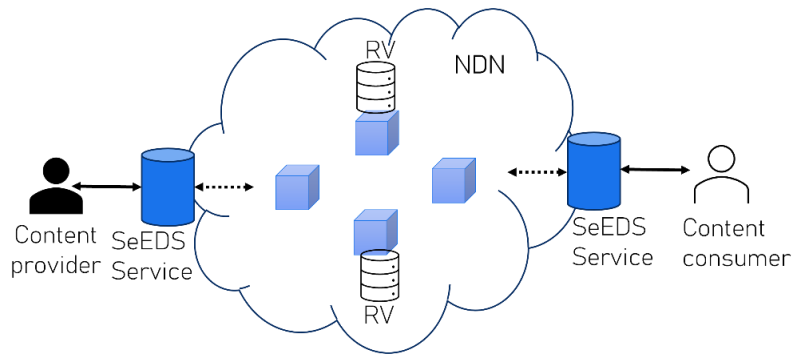
\includegraphics[width=0.8\linewidth]{images/seeds_architecture.png}
    \caption{High level SeEDS architecture.}
    \label{fig:seeds_architecture}
\end{figure}

\pagebreak

The following is the SeEDS Service components in detail: 

\begin{figure}[H]
    \centering
    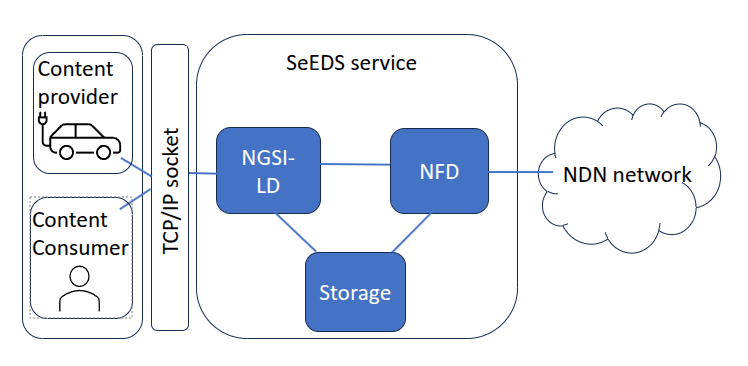
\includegraphics[width=0.8\linewidth]{images/seeds_service_detail.png}
    \caption{SeEDS Service in detail.}
    \label{fig:seeds_service_detail}
\end{figure}

The current architecture enables the SeEDS Service to perform the following operations: 

\begin{itemize}
    \item Consumers can create a \textit{HTTP GET} request to retrieve items from the NDN network. As mentioned before these are either \emph{GET by TYPE} or {GET by ID}. Note that the \textit{@type} and \textit{@id} need to be provided accordingly. 
    \item Providers can create \textit{HTTP POST} requests to provide/announce items to the NDN network. The service will also ensure that the data is stored inside its storage, ensuring that the data can be served when requested from some other node in the network. 
    \item Clients can also subscribe to a specific \textit{@id} or \textit{@type}. Since content in NDN is retrieved by its unique name rather than by host address, clients may express a request for a name even before the corresponding data is available. Once the data is published under that name, the network delivers it to all subscribed clients, enabling efficient and timely notifications.
    \item The NDN naming scheme also enables any NDN node to act as a \emph{Secondary} for another node within the network. A \emph{Secondary} node inherits the data of its corresponding \emph{Primary} node, including its storage contents, announced \textit{@ids}, \textit{@types} and \textit{subscriptions}. This design enhances the resilience of the SeEDS system, allowing it to recover the data of a failed node seamlessly and maintain service continuity.
\end{itemize}

\subsection{Resilience}

The resilience layer in SeEDS ensures that a \emph{Secondary} node continuously converges towards the state of a \emph{Primary} node through lightweight synchronization protocols built on NDN. At the core of this mechanism lies a versioned canonical JSON store on the \emph{Primary}, which exposes its state through a set of standardized NDN Interests and Data packets. The \emph{Secondary} maintains a local mirror of this store, applying updates received from the network and validating them against deterministic fingerprints.

The \emph{Primary} store maintains a bounded history of mutations. Each change increments a version counter, recomputes a canonical hash of the entire state, and records a snapshot to support future patch generation. It responds to queries with one of three data views: a lightweight metadata descriptor containing only the version and hash; a delta, represented as an RFC 6902 JSON Patch from one version to another; or a full snapshot of the canonical state. The \emph{Secondary} mirror accepts these responses and applies them locally. Whenever patch application fails, or when the requested patch is unavailable, the mirror falls back to a snapshot, ensuring eventual consistency even in the presence of divergence.

The resilience system is designed to handle failures gracefully. If the poller records consecutive failures in its liveness probes that exceed a configurable threshold, the \emph{Secondary} promotes itself to \emph{Primary} and terminates the polling loop. This self-promotion is communicated to the local services through IPC, ensuring that the system can continue to operate without interruption despite the failure of the original \emph{Primary}.

\begin{figure}[H]
    \centering
    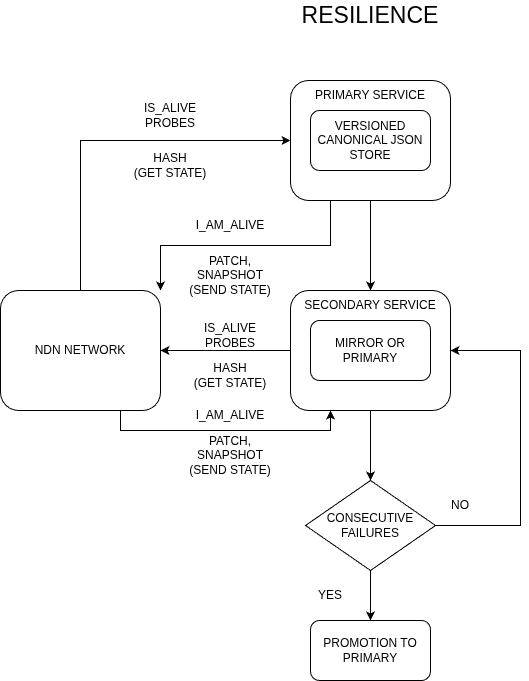
\includegraphics[width=0.8\linewidth]{images/resilience_seeds.png}
    \caption{Resilience architecture in SeEDS.}
    \label{fig:resilience_architecture}
\end{figure}

\section{Implementation}

The implementation described in this section reflects the state of the SeEDS system as of October 2025. As the project continues to evolve, certain design choices, component interfaces, or architectural details may change to accommodate new requirements, optimizations, or future redesigns. Therefore, this documentation should be considered a snapshot of the current implementation rather than a definitive or final version.


\subsection{Announcing Content}

When a node intends to announce content within the NDN network, it does so by advertising specific names. Consumers can then retrieve the corresponding content by \emph{expressing Interests} for these names. Each node in the network possesses a unique identifier (e.g., Node~1 on the left and Node~2 on the right). As illustrated in messages \emph{(0)} and \emph{(1)}, each node initially announces the base \textit{SeEDS} name concatenated with its unique identifier, forming the name \textit{SeEDS\textunderscore ID}. In addition, each node announces a \emph{scope} under a name of the form \textit{ID\textunderscore scopeID}. If a node is responsible for a particular registry or entity type—such as the \textit{CAR\textunderscore registry} in this example, shown in messages \emph{(2)} and \emph{(3)} —it also advertises the corresponding \textit{TYPE} and \textit{TYPE\textunderscore REGISTRY} names, enabling it to respond to Interests related to that registry.

\begin{figure}[H]
    \centering
    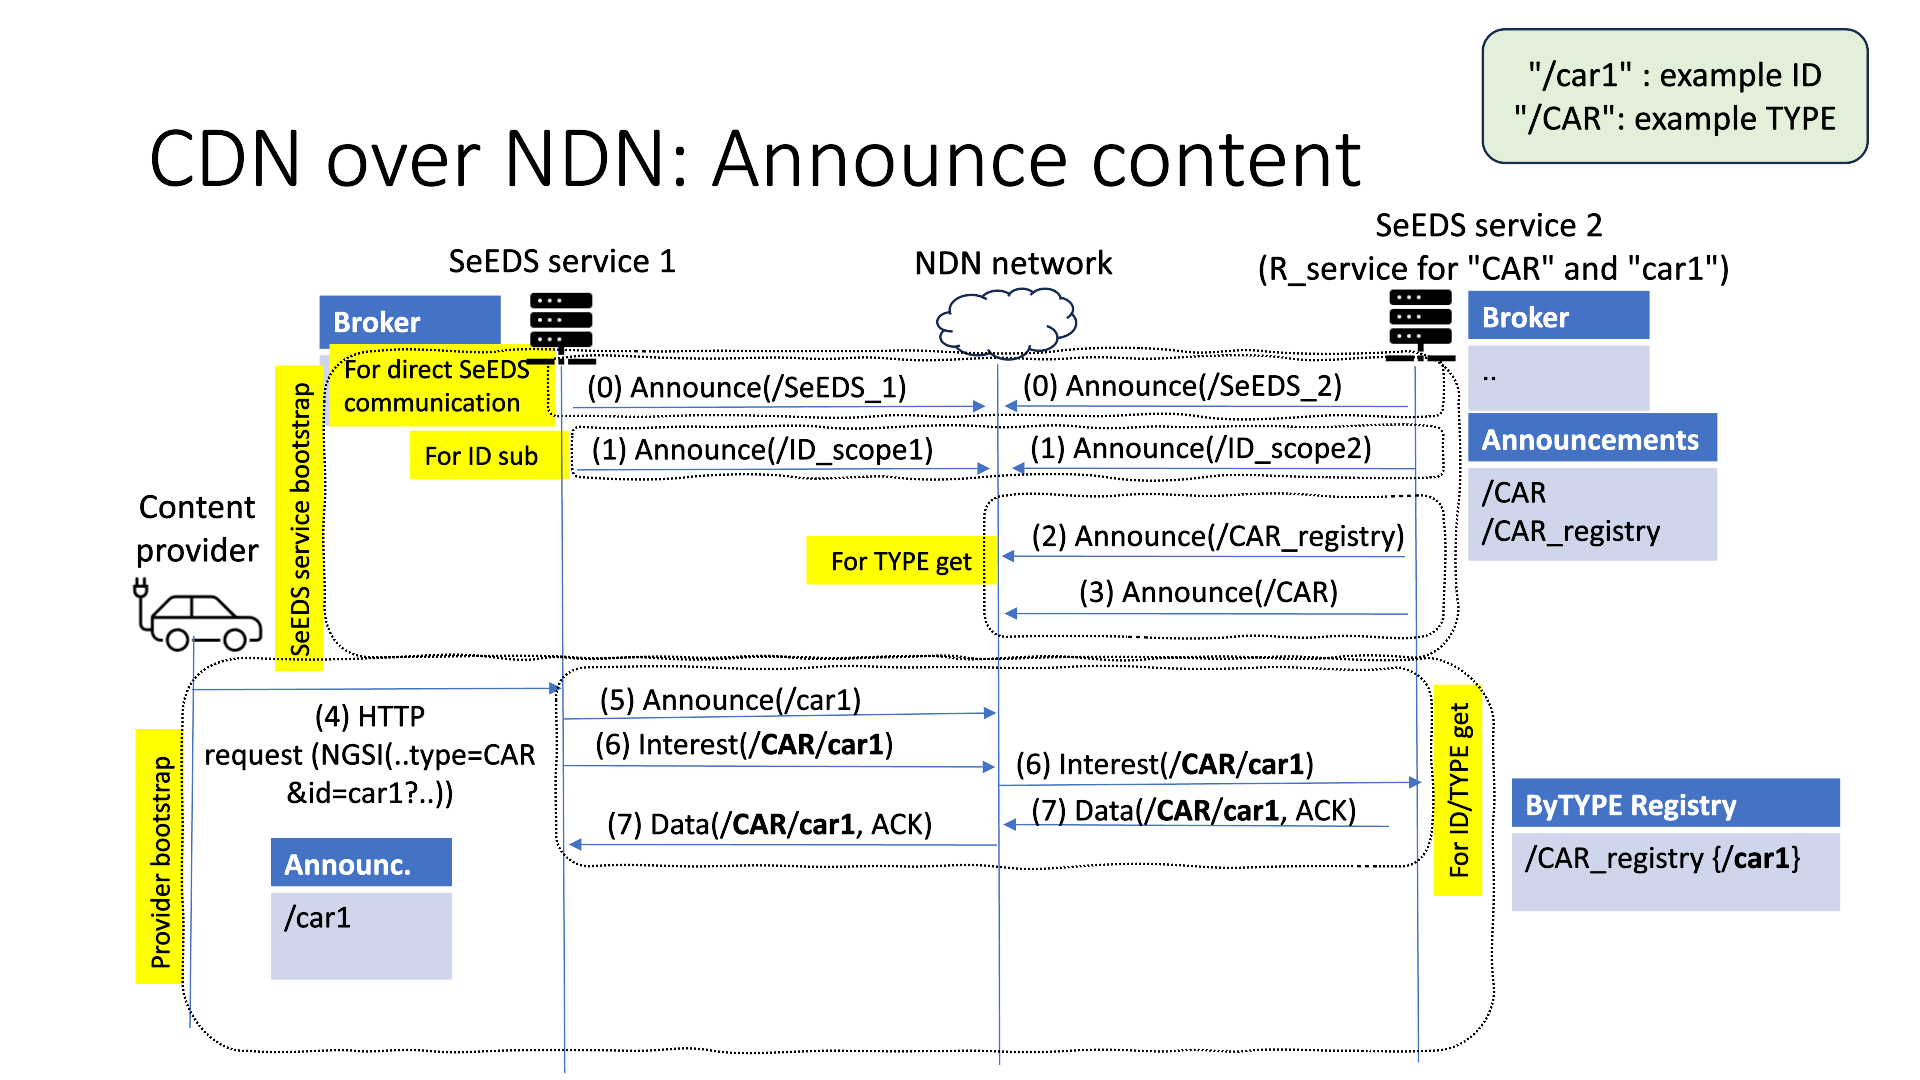
\includegraphics[width=0.8\linewidth]{images/announce_content.png}
    \caption{Announcing content inside the NDN network.}
    \label{fig:annoucing_content}
\end{figure}

Following the initial announcements, a new client intends to provide an entity with \textit{@id = car1} of type \textit{@type = CAR}. When this new \textit{@id} arrives, the receiving SeEDS Service first announces it locally, as illustrated in message~\emph{(5)}. It must then \emph{express an Interest}, as shown in message~\emph{(6)}, for the \textit{@type = CAR} registry so that the responsible node can store the new entry in the registry. The responsible node replies with an \emph{ACK} message, confirming that \textit{@id = car1} has been successfully registered under \textit{@type = CAR}. If the client’s \emph{HTTP request} does not explicitly specify a \textit{@type}, the system omits messages~\emph{(6)} and~\emph{(7)} and only announces the \textit{@id = car1} within the network.

\subsection{GET by ID}\label{get_by_id_section}



After an \textit{@id} is published into the network users can retrieve its content. Users create an \emph{HTTP Request} and specify the \textit{@id} that they want to retrieve, as shown in message \emph{(0)}. The SeEDS Service processes the message internally and \emph{expresses an interest} involving the \textit{@id=car1} inside the name, as shown in message \emph{(1)}. Note that messages~\emph{(0)} and~\emph{(1)} are identical in both the \emph{Direct} and \emph{Indirect} modes of the \texttt{GET by ID} operation. The choice of modes occurs dynamically depending on the data received by \textit{ProcessQueries()}. Moreover in both \emph{Direct} and \emph{Indirect} modes, the processing of filters occurs before the final data is returned to the user via the HTTP interface. Only the fields explicitly specified in the filter conditions are retained in the output. 


\subsubsection{Direct Mode}

\emph{Direct mode} occurs when the data processed by \textit{ProcessQueries()} is classified as a \emph{small payload}. In this case, the SeEDS Service responsible for the corresponding \textit{@id} responds \emph{directly} with the JSON payload, as illustrated in message~\emph{(2)}. The SeEDS Service that initially received the \emph{HTTP request} then forwards this data back to the client as the final response.

\begin{figure}[H]
    \centering
    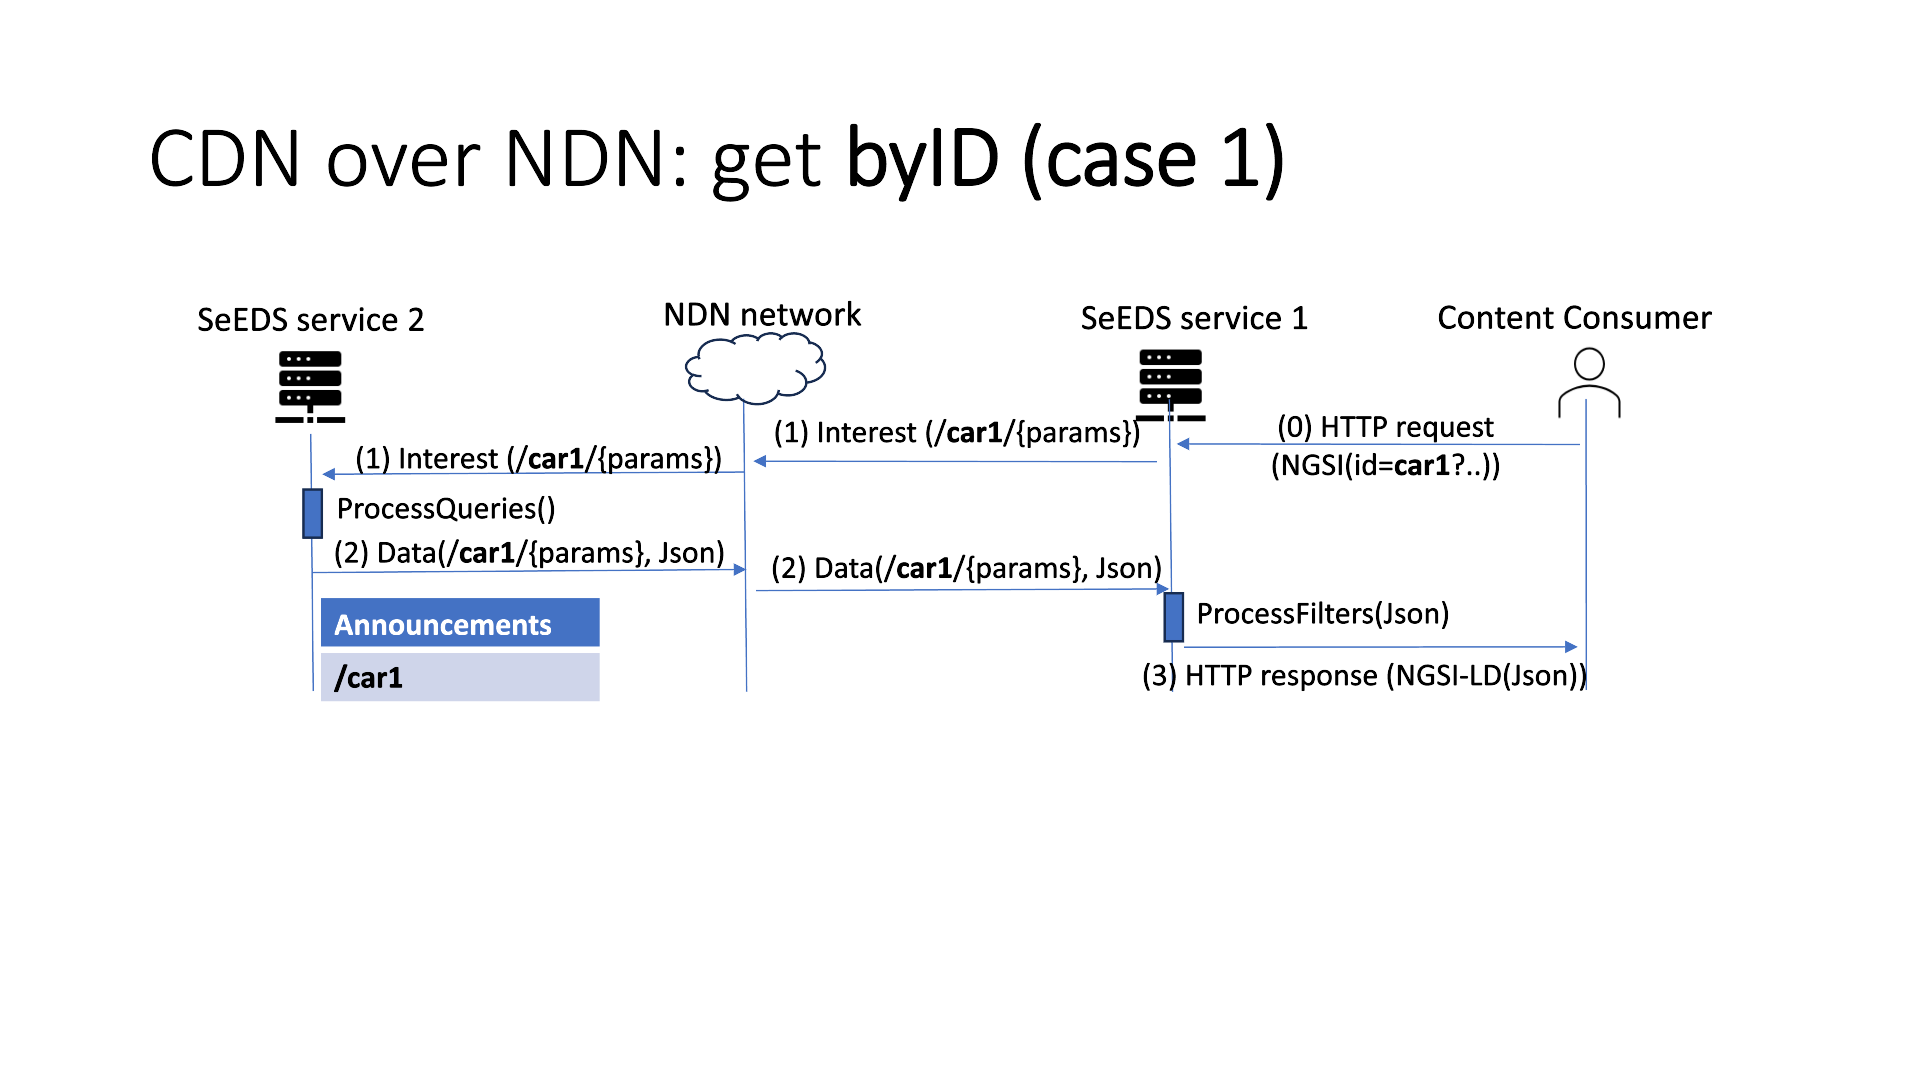
\includegraphics[width=0.8\linewidth]{images/get_by_id_direct.png}
    \caption{GET by ID direct mode.}
    \label{fig:get_by_id_direct}
\end{figure}

\subsubsection{Indirect Mode}

\emph{Indirect mode} occurs when the data processed by \textit{ProcessQueries()} is classified as a \emph{large payload}. In this case, the SeEDS Service responsible for the corresponding \textit{@id} does not transmit the full JSON directly. Instead, it responds with a \emph{metafile}, as illustrated in message~\emph{(2)}. The \emph{metafile} contains a list of \textit{@v\_ids}, which represent the individual \textit{@ids} along with their respective versions. Upon receiving the \emph{metafile}, the SeEDS Service that originally handled the \emph{HTTP request} proceeds to \emph{express Interests} for the specific \textit{@id} and each associated version. This effectively reinitiates the retrieval process in the same manner as a \emph{Direct mode} request, just for a specific version. The version can be represented in various forms, such as a timestamp, a numerical identifier, or any other scheme that uniquely distinguishes different instances of the same entity.


\begin{figure}[H]
    \centering
    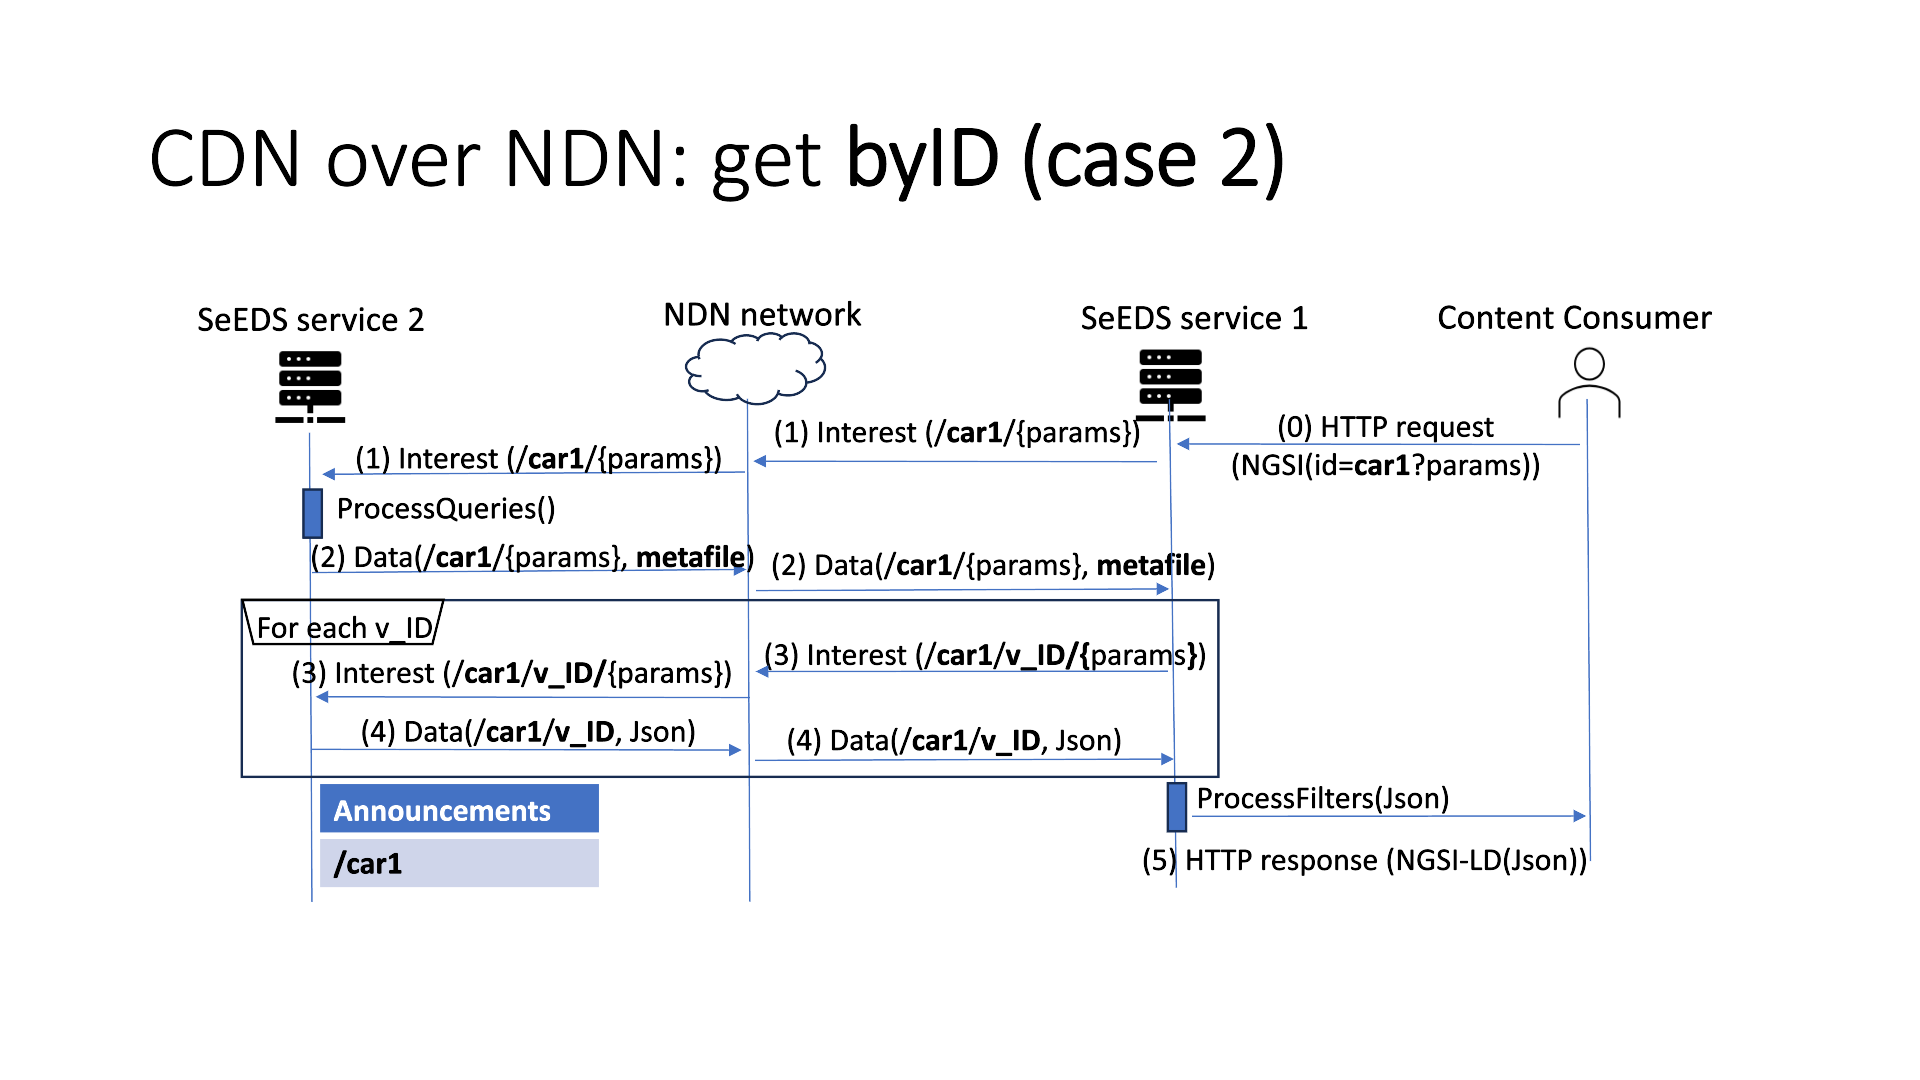
\includegraphics[width=0.8\linewidth]{images/get_by_id_indirect.png}
    \caption{GET by ID indirect mode.}
    \label{fig:get_by_id_indirect}
\end{figure}

\pagebreak 

\subsection{GET by TYPE}\label{get_by_type_section}

Users can also request data associated with a specific \textit{@type}. As illustrated in message~\emph{(0)}, the \emph{content consumer} specifies the desired \textit{@type} in the request sent to the SeEDS Service. The SeEDS Service that receives the \emph{HTTP Request} proceeds to \emph{express an Interest} in the NDN network, as shown in message~\emph{(1)}. The SeEDS Service responsible for the corresponding registry then receives this Interest and responds with the list of \textit{@ids} registered under that \textit{@type}, as shown in message~\emph{(2)}. After obtaining the list of \textit{@ids}, the SeEDS Service that originally handled the \emph{HTTP request} performs a separate \hyperref[get_by_id_section]{GET by ID} operation for each \textit{@id} to retrieve the associated data.

\begin{figure}[H]
    \centering
    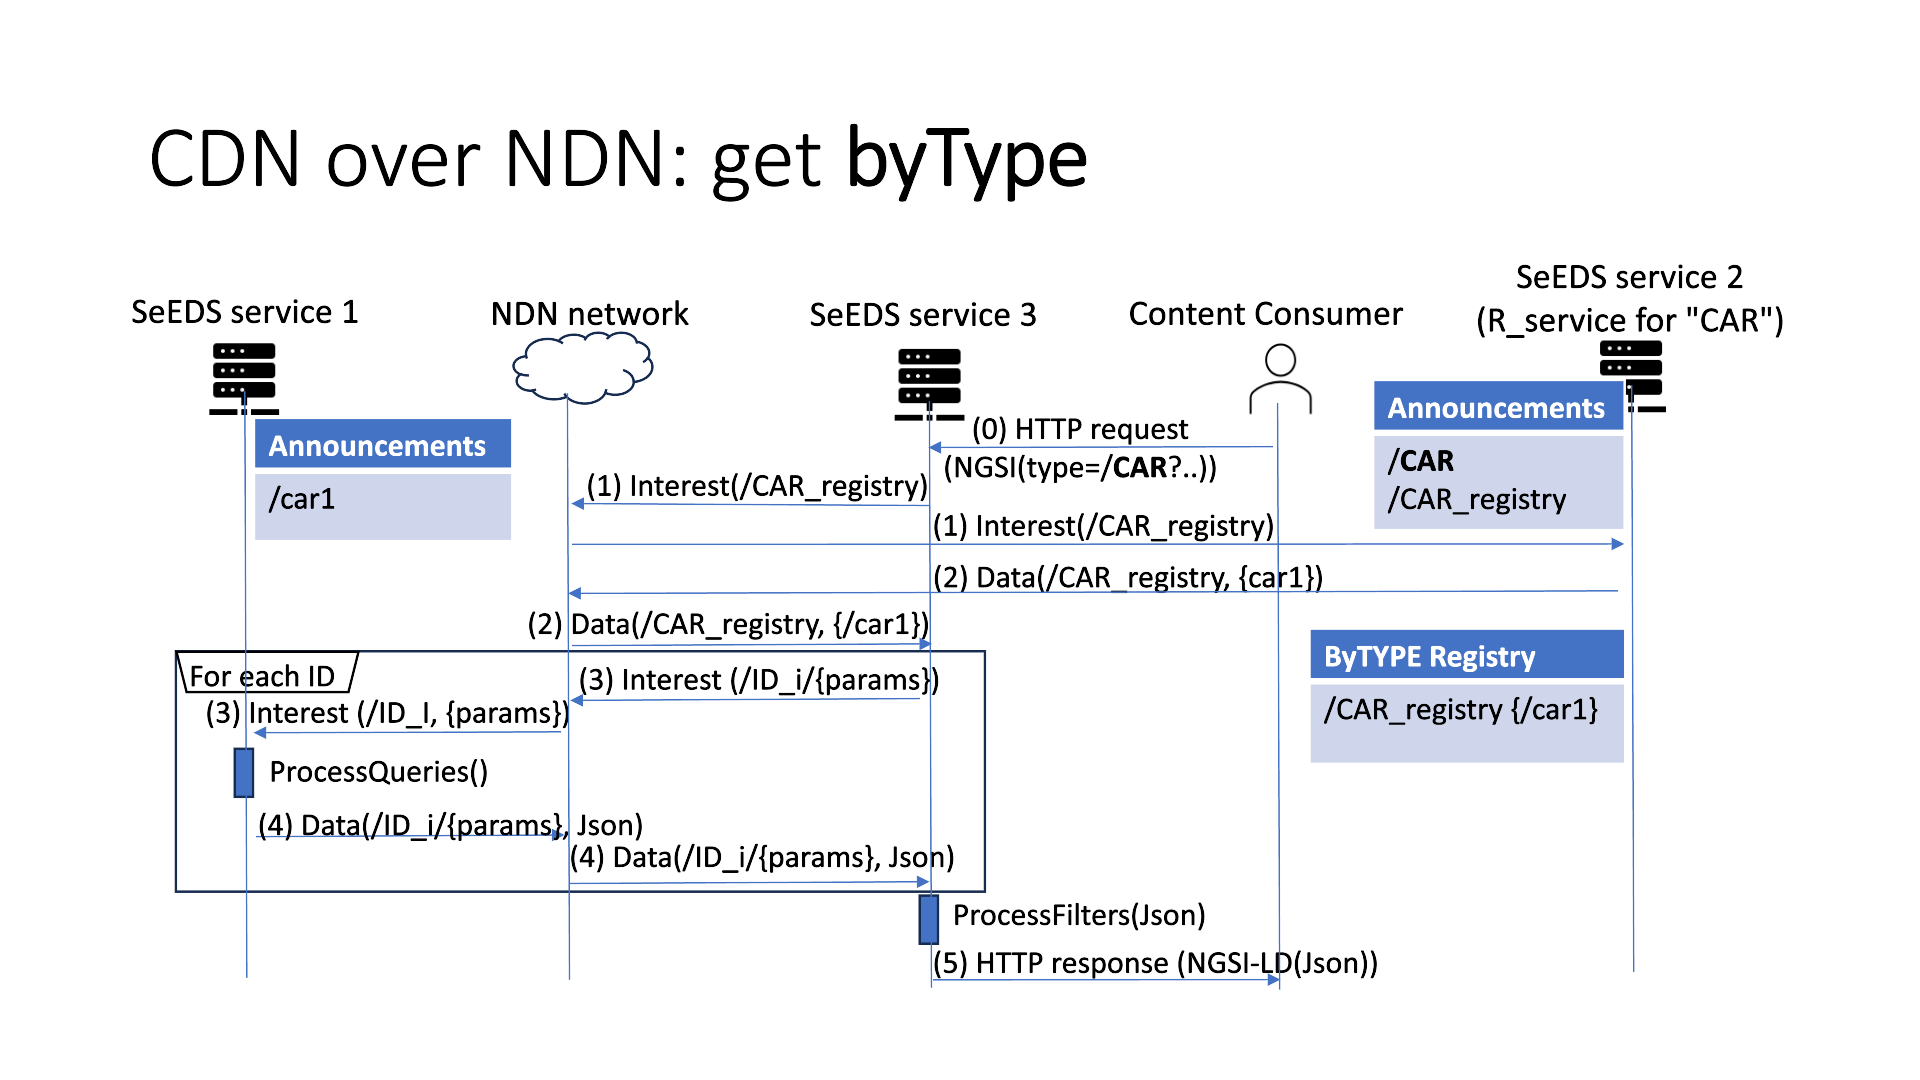
\includegraphics[width=0.8\linewidth]{images/get_by_type.png}
    \caption{GET by TYPE.}
    \label{fig:get_by_type}
\end{figure}

\pagebreak

\subsection{SUBSCRIPTIONS by ID}\label{subscriptions_by_id_section}

Consumers can also subscribe to a specific \textit{@id}. Once content associated with that \textit{@id} becomes available, the system automatically notifies the subscribed consumers and delivers the corresponding data. This mechanism allows consumers to subscribe to \textit{@ids} even before the data has been published. 

A consumer that wishes to subscribe to an \textit{@id} must specify the target identifier, as illustrated in message~\emph{(0)}. Upon receiving the \emph{HTTP request}, the SeEDS Service proceeds to \emph{express an Interest} containing both the responsible \emph{ID\_SCOPEID} for the given \textit{@id}—determined via a hashing function—and its own \emph{ID\_SCOPEID}, as shown in message~\emph{(1)}. When the responsible \emph{ID\_SCOPEID} receives this Interest, it records the sender’s \emph{ID\_SCOPE} as a subscriber for the specified \textit{@id} and responds with an \emph{ACK}, as depicted in message~\emph{(2)}.

When new data for the subscribed \textit{@id} is announced, the system checks for any existing subscribers and notifies them through their respective scopes that new content has become available, as shown in message~\emph{(3)}. The notified SeEDS Service then initiates a \hyperref[get_by_id_section]{GET by ID} operation to retrieve the newly published data.

\begin{figure}[H]
    \centering
    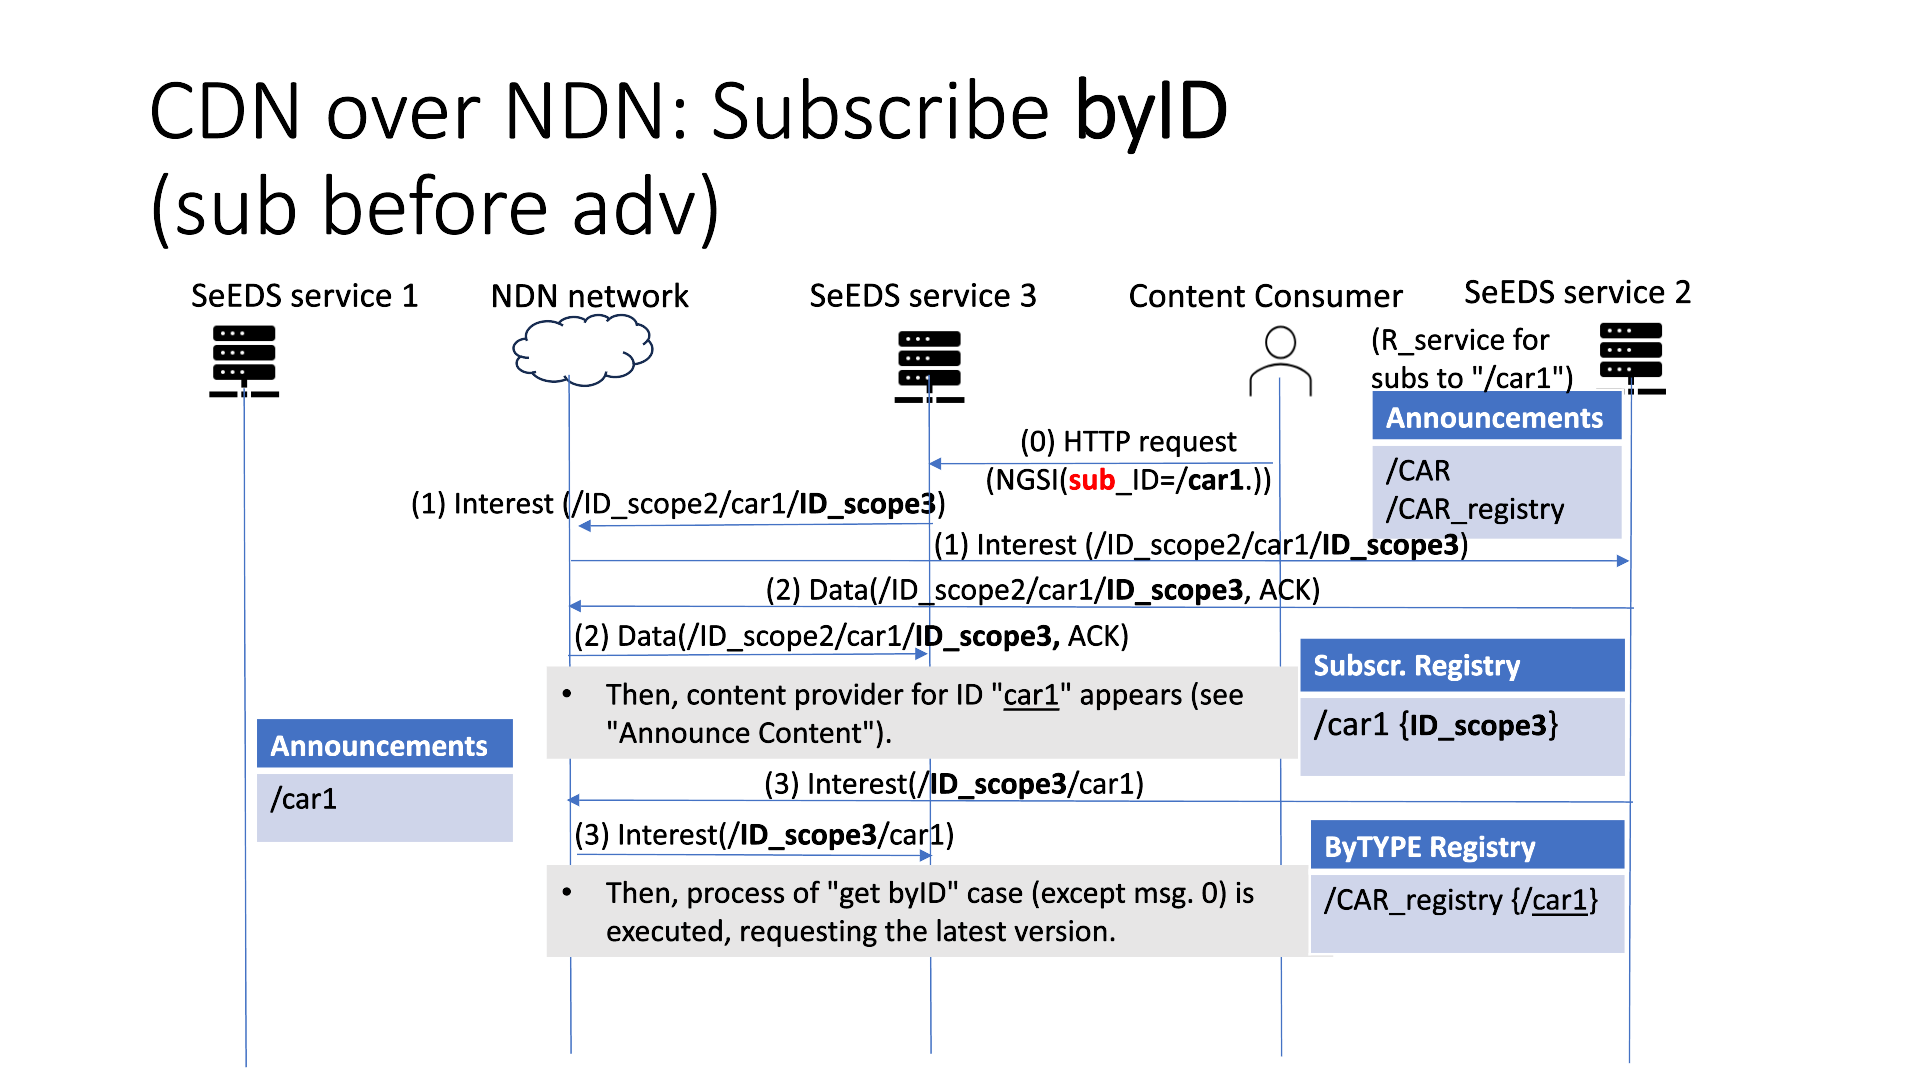
\includegraphics[width=0.8\linewidth]{images/subscribe_by_id.png}
    \caption{Subscribe by ID.}
    \label{fig:subscribe_by_id}
\end{figure}

\subsection{SUBSCRIPTIONS by TYPE}

Consumers can also subscribe to a specific \textit{@type}. In this case ( unlike \hyperref[subscriptions_by_id_section]{SUBSCRIBE by ID} ) , the subscription is linked to an already announced registry scope, so there is no need to compute a hash for the \textit{@type}. When the registry receives new data entries for that \textit{@type}, all subscribed consumers are notified that an update has occurred. 

As shown in message~\emph{(0)}, the consumer specifies the target \textit{@type} in the \emph{HTTP Request} sent to the SeEDS Service. Upon receiving the \emph{HTTP request}, the SeEDS Service expresses an \emph{Interest} toward the corresponding registry scope associated with that \textit{@type}, as illustrated in message~\emph{(1)}. The registry records the SeEDS Service that issued the Interest as a subscriber ( the diagram doesn't use \emph{ID\_SCOPE} but \emph{SeEDS\_ID} which is equivalent ) and replies with an \emph{ACK}, confirming that the subscription has been successfully registered, as shown in message~\emph{(2)}.

When new data is added to the registry for the subscribed \textit{@type}, the system notifies all registered subscribers, as depicted in message~\emph{(3)}. Upon receiving the notification, the SeEDS Service proceeds to perform a \hyperref[get_by_type_section]{GET by TYPE} operation to retrieve the updated content.


\begin{figure}[H]
    \centering
    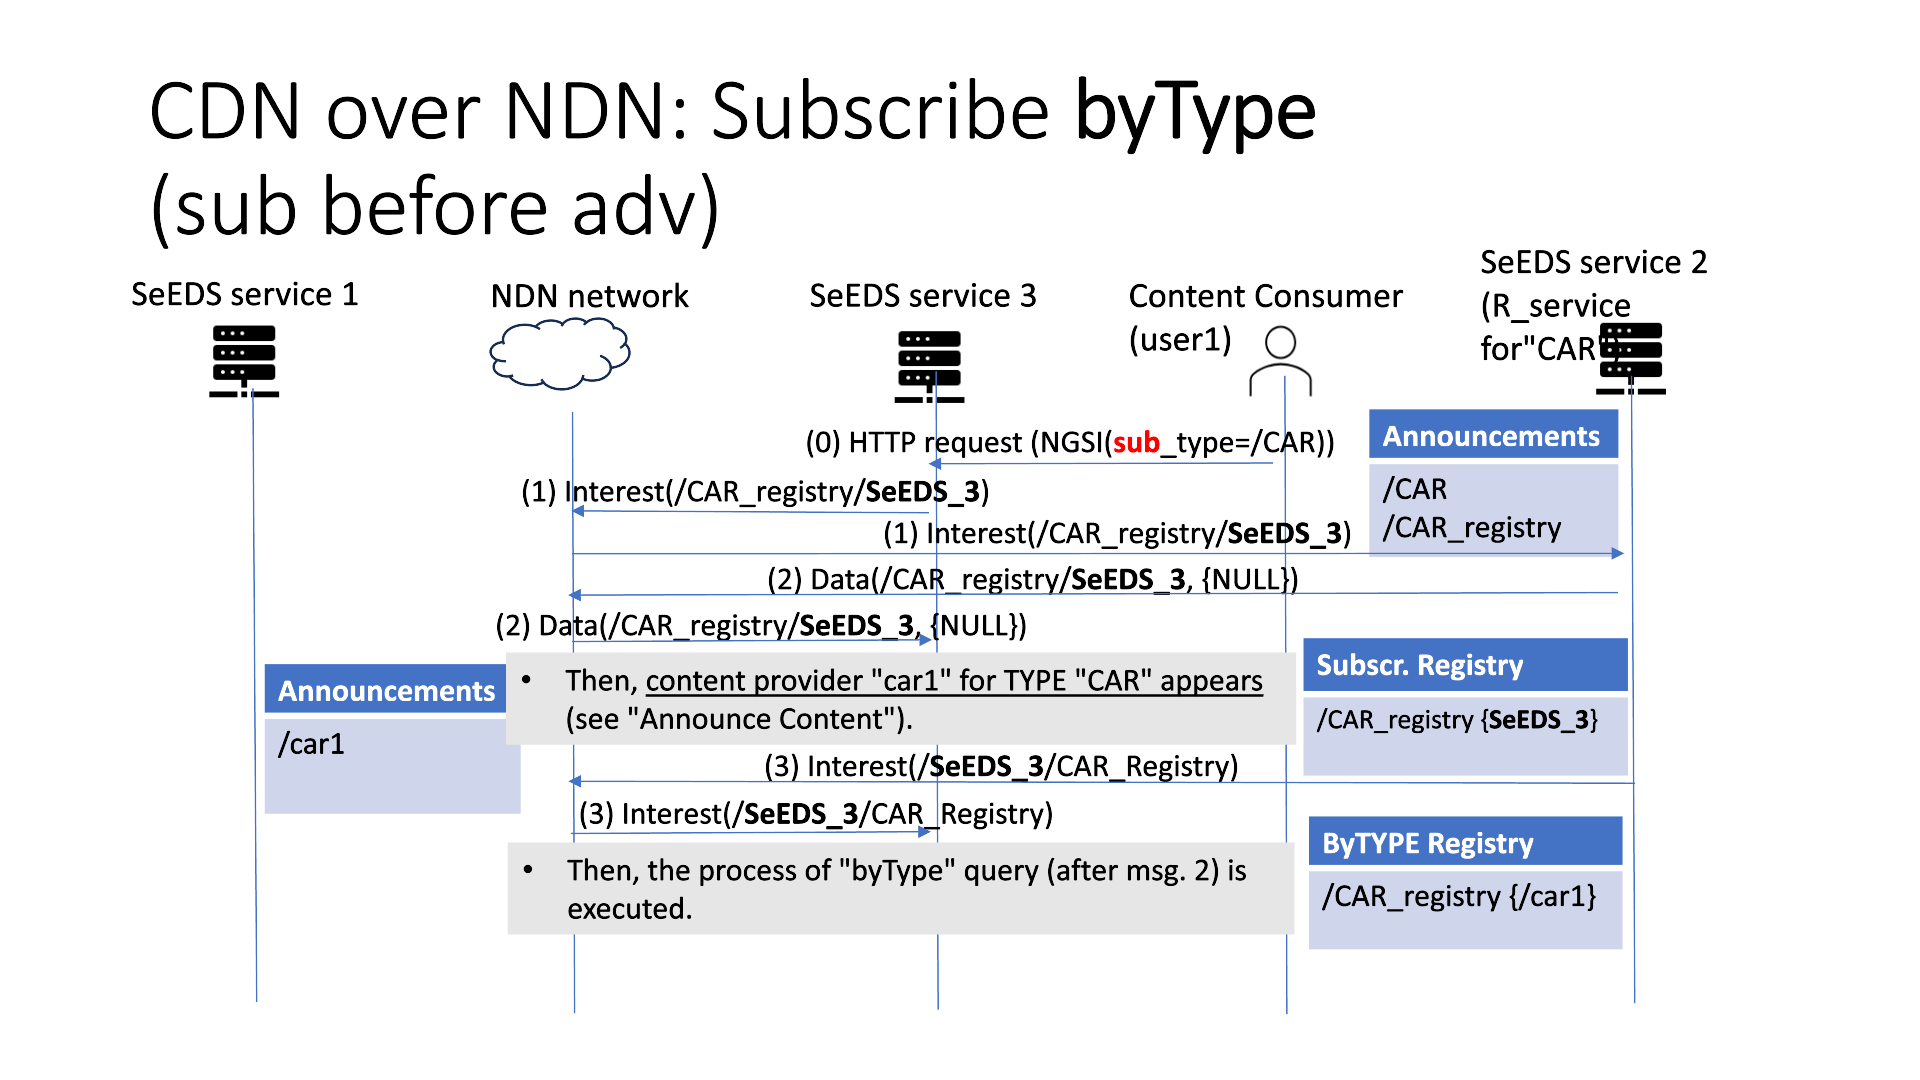
\includegraphics[width=0.8\linewidth]{images/subscribe_by_type.png}
    \caption{Subscribe by type.}
    \label{fig:subscribe_by_type}
\end{figure}

\pagebreak 

\subsection{Resilience}

Figure~\ref{fig:resilience} illustrates the message exchange that keeps a \emph{Secondary} SeEDS service converged with a remote \emph{Primary} over the NDN network. The \emph{Secondary} (left lane) runs two lightweight polling loops in parallel: (i) a \emph{state convergence} loop that tracks the \textit{state} of the Primary’s canonical store, and (ii) a \emph{liveness} loop that verifies that the remote service is responsive. Both loops use standardized Interests and Data packets and carry only minimal material (hashes, patches-snapshots, nonces) to limit overhead.

As shown in message~\emph{(0)}, the Primary has announced its state namespace \texttt{\{state\_2\}} in the NDN network, so other Services in the network can \emph{express interests} for it. The currently manually set Secondary initiates its state convergence loop by expressing an \emph{Interest} for the corresponding state hash, as depicted in message~\emph{(2)}. The returned \emph{Data} packet, shown in message~\emph{(3)}, contains the current hash and either a patch encoded as an RFC~6902 JSON Patch or an RFC~6902 Snapshot. The Secondary compares this hash with the locally stored version, and when a mismatch is detected, it applies the received patch or the snapshot, if the patch cannot be applied, to synchronize its local mirror with the Primary. 

Parallel to the state convergence loop, the Secondary executes a liveness verification loop to confirm that the Primary remains reachable. As illustrated in message~\emph{(1)}, the Primary advertises its liveness namespace \texttt{\{is\_alive\_2\}}. The Secondary periodically expresses \emph{Interest} packets containing a fresh nonce, as shown in message~\emph{(4)}. The Primary responds with a corresponding \emph{Data} packet that echoes the nonce and includes an acknowledgment, as depicted in message~\emph{(5)}. 

If the Secondary records consecutive failures in its liveness probes beyond a predefined threshold, it promotes itself to the \emph{Primary} and terminates the polling loop. This promotion is internally communicated to the SeEDS services through IPC, ensuring that operation continues uninterrupted even in the absence of the original Primary. This mechanism, SeEDS achieves distributed fault tolerance, maintaining service availability despite network or node failures.

\begin{figure}[H]
    \centering
    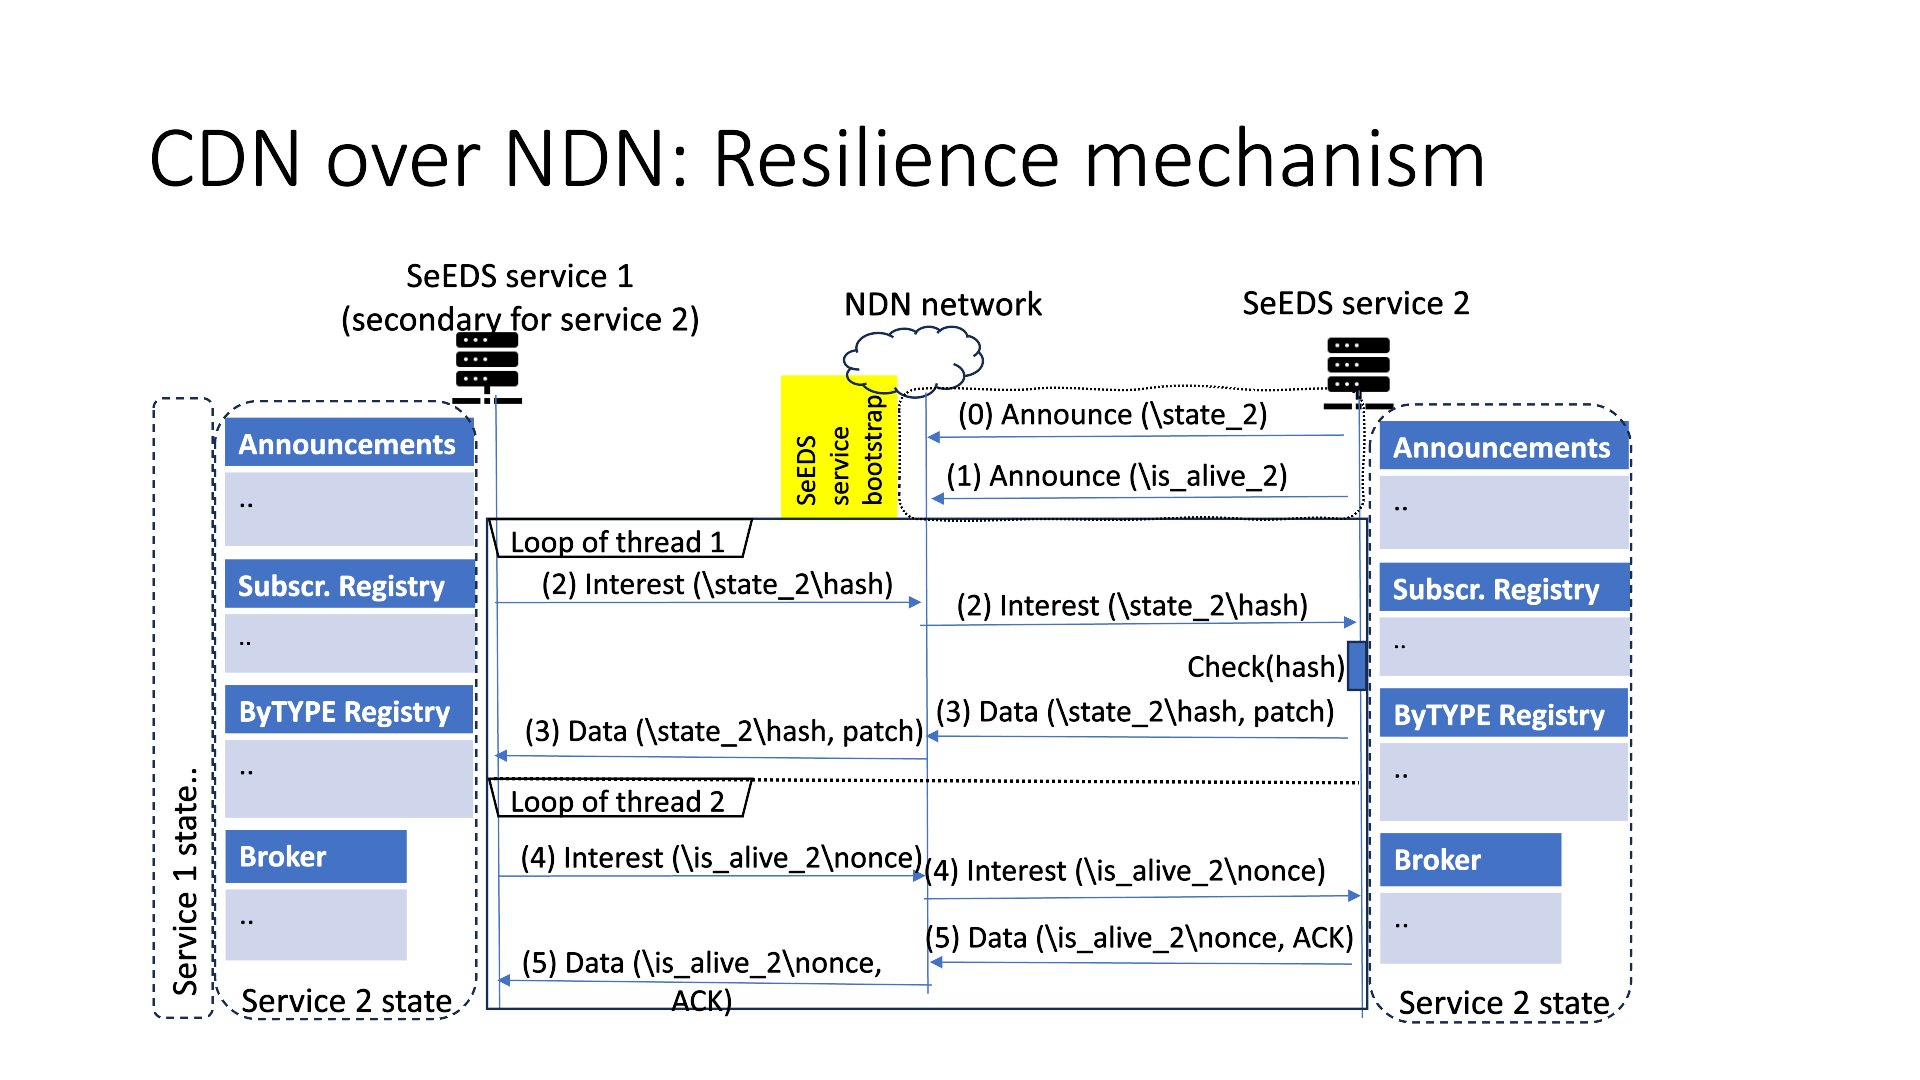
\includegraphics[width=0.8\linewidth]{images/resilience.png}
    \caption{Resilience message exchange in SeEDS.}
    \label{fig:resilience}
\end{figure}

\section{Experiments and KPIs}

\subsection{MiniNDN evalution}

Mini-NDN is a lightweight emulation framework designed to facilitate experimentation with Named Data Networking (NDN) in a controlled, reproducible environment. It is built on top of \textit{Mininet}, a popular network emulator that allows users to create virtual network topologies composed of multiple nodes, links, and switches within a single physical or virtual machine. Mini-NDN extends this capability by integrating the NDN Forwarding Daemon (NFD) and NDN tools into each emulated node, effectively transforming the Mininet network into a fully functional NDN deployment.

Each Mini-NDN node runs its own instance of NFD and can host NDN applications, such as producers and consumers, enabling realistic Interest/Data exchange over emulated network topologies. Mini-NDN supports custom configurations through topology and configuration files, making it straightforward to define arbitrary network graphs and specify per-node parameters such as faces, prefixes, and routing protocols.

Mini-NDN was employed to test and validate the functionality of the SeEDS prototype prior to its deployment in the global NDN testbed, ensuring correct operation before deployment to the actual testbed. Below, for brevity's sake, we are going to present the basic \emph{GET by ID} and \emph{GET by TYPE} requests. Everything else has been tested to ensure its correct operation and can be found on the \href{https://github.com/mmlab-aueb/SeEDS/blob/main/README.md}{official github repository}( \textbf{KPI 9} ).


\subsubsection{Topology}

The Mini-NDN emulation was deployed using a simple four-node topology defined in the configuration file shown in Listing~\ref{lst:minindn_conf}. The nodes are labeled \texttt{a}, \texttt{b}, \texttt{c}, and \texttt{d}, each running its own instance of the NDN Forwarding Daemon (NFD) with the log level set to \texttt{DEBUG}.

The connectivity between nodes is symmetric, with bidirectional links defined for each pair. Nodes \texttt{a}, \texttt{b}, and \texttt{c} form a triangular core interconnected with a delay of \texttt{10\,ms} per link, ensuring low-latency communication suitable for multi-hop experiments. Node \texttt{d} connects only to node \texttt{a}, also with a \texttt{10\,ms} delay, representing an edge node that communicates with the core through a single gateway.

\begin{figure}[H]
\centering
\begin{tikzpicture}[
    node/.style={circle, draw, thick, minimum size=9mm, font=\sffamily\bfseries},
    link/.style={-{Stealth[length=2mm]}-{Stealth[length=2mm]}, thick},
    >=Stealth
]
% Nodes
\node[node] (a) at (0,0) {a};
\node[node] (b) at (4,0) {b};
\node[node] (c) at (2,3) {c};
\node[node] (d) at (-2,0) {d};

% Core triangle links (bidirectional, 10 ms)
\draw[link] (a) -- node[above left,pos=0.5]{\small 10\,ms} (c);
\draw[link] (b) -- node[above right,pos=0.5]{\small 10\,ms} (c);
\draw[link] (a) -- node[below,pos=0.5]{\small 10\,ms} (b);

% Edge link for d (to a only)
\draw[link] (d) -- node[below,pos=0.5]{\small 10\,ms} (a);


\end{tikzpicture}
\caption{Mini-NDN topology: triangular core (a–b–c) with 10\,ms links; edge node d connected to a.}
\label{fig:minindn_topology}
\end{figure}

\begin{lstlisting}[language=minindnconf,caption={Mini-NDN topology .conf file},label={lst:minindn_conf}]
[nodes]
a: _ nfd-log-level=DEBUG
b: _ nfd-log-level=DEBUG
c: _ nfd-log-level=DEBUG
d: _ nfd-log-level=DEBUG

[links]
a:b delay=10ms
b:a delay=10ms
b:c delay=10ms
c:b delay=10ms
c:a delay=10ms
a:c delay=10ms
d:a delay=10ms
a:d delay=10ms
\end{lstlisting}


\pagebreak 

\subsubsection{GET by ID}

We have already published the \textit{@ids=car1,car2,car3} in the NDN network, through \emph{node A ( producer )}.


Let's try to retrieve the \textit{@id=car1} through \emph{node B}:

\begin{lstlisting}[language=log, caption={Node's B log after performing a GET by ID for car1}, label={lst:node-b-log-file-car1}]
[2025-09-25 00:33:40.583] [debug] [Consumer] Extracted content from message: /SNDS/car1/getByID:car1
[2025-09-25 00:33:40.583] [debug] [Consumer] Extracted content length from message: 23
[2025-09-25 00:33:40.583] [debug] [Consumer] Extracted message type from message: GET_BY_ID_REQUEST
[2025-09-25 00:33:40.583] [debug] [Consumer] Query.type: 
[2025-09-25 00:33:40.583] [debug] [Consumer] Query.id: car1
[2025-09-25 00:33:40.583] [info] [Consumer] Created name /SNDS/car1/temporalQuery:id%3Dcar1&type%3D&date%3D&count%3D&timeframe%3D&filters%3D
[2025-09-25 00:33:40.583] [info] [Consumer] Sending actual Interest /SNDS/car1/temporalQuery%3Aid%3Dcar1%26type%3D%26date%3D%26count%3D%26timeframe%3D%26filters%3D?CanBePrefix&Lifetime=6000
[2025-09-25 00:33:40.585] [info] [Consumer] Received Data with name: /SNDS/car1/temporalQuery%3Aid%3Dcar1%26type%3D%26date%3D%26count%3D%26timeframe%3D%26filters%3D in function onData
[2025-09-25 00:33:40.585] [info] [Consumer] Data packet payload: [
  {
    "": {
      "_id": "car1",
      "id": "car1",
      "timestamp": {
        "$date": 1758749528574
      },
      "type": "GENERIC"
    }
  }
] in function onData
[2025-09-25 00:33:40.585] [info] [Consumer] Parsed interest: Prefix: SNDS, Name: car1, Command: temporalQuery, Params: [id=car1, type=, date=, count=, timeframe=, filters=] in onData
[2025-09-25 00:33:40.585] [info] [Consumer] Temporal Query Reponse... 
\end{lstlisting}

\pagebreak 

Let's try to retrieve the \textit{@id=car2} through \emph{node C}:
\begin{lstlisting}[language=log, caption={Node's C log after performing a GET by ID for car2}, label={lst:node-c-log-file-car2}]
[2025-09-25 00:42:10.775] [debug] [Consumer] Extracted content from message: /SNDS/car2/getByID:car2
[2025-09-25 00:42:10.775] [debug] [Consumer] Extracted content length from message: 23
[2025-09-25 00:42:10.775] [debug] [Consumer] Extracted message type from message: GET_BY_ID_REQUEST
[2025-09-25 00:42:10.775] [debug] [Consumer] Query.type: 
[2025-09-25 00:42:10.775] [debug] [Consumer] Query.id: car2
[2025-09-25 00:42:10.775] [info] [Consumer] Created name /SNDS/car2/temporalQuery:id%3Dcar2&type%3D&date%3D&count%3D&timeframe%3D&filters%3D
[2025-09-25 00:42:10.775] [info] [Consumer] Sending actual Interest /SNDS/car2/temporalQuery%3Aid%3Dcar2%26type%3D%26date%3D%26count%3D%26timeframe%3D%26filters%3D?CanBePrefix&Lifetime=6000
[2025-09-25 00:42:10.777] [info] [Consumer] Received Data with name: /SNDS/car2/temporalQuery%3Aid%3Dcar2%26type%3D%26date%3D%26count%3D%26timeframe%3D%26filters%3D in function onData
[2025-09-25 00:42:10.777] [info] [Consumer] Data packet payload: [
  {
    "": {
      "_id": "car2",
      "id": "car2",
      "timestamp": {
        "$date": 1758749532578
      },
      "type": "GENERIC"
    }
  }
] in function onData
[2025-09-25 00:42:10.777] [info] [Consumer] Parsed interest: Prefix: SNDS, Name: car2, Command: temporalQuery, Params: [id=car2, type=, date=, count=, timeframe=, filters=] in onData
\end{lstlisting}

\pagebreak

Let's try to retrieve the \textit{@id=car3} through \emph{node D}:
\begin{lstlisting}[language=log, caption={Node's D log after performing a GET by ID for car3}, label={lst:node-d-log-file-car3}]
[2025-09-25 00:38:19.399] [debug] [Consumer] Extracted content from message: /SNDS/car3/getByID:car3
[2025-09-25 00:38:19.399] [debug] [Consumer] Extracted content length from message: 23
[2025-09-25 00:38:19.399] [debug] [Consumer] Extracted message type from message: GET_BY_ID_REQUEST
[2025-09-25 00:38:19.399] [debug] [Consumer] Query.type: 
[2025-09-25 00:38:19.399] [debug] [Consumer] Query.id: car3
[2025-09-25 00:38:19.399] [info] [Consumer] Created name /SNDS/car3/temporalQuery:id%3Dcar3&type%3D&date%3D&count%3D&timeframe%3D&filters%3D
[2025-09-25 00:38:19.399] [info] [Consumer] Sending actual Interest /SNDS/car3/temporalQuery%3Aid%3Dcar3%26type%3D%26date%3D%26count%3D%26timeframe%3D%26filters%3D?CanBePrefix&Lifetime=6000
[2025-09-25 00:38:19.400] [info] [Consumer] Received Data with name: /SNDS/car3/temporalQuery%3Aid%3Dcar3%26type%3D%26date%3D%26count%3D%26timeframe%3D%26filters%3D in function onData
[2025-09-25 00:38:19.400] [info] [Consumer] Data packet payload: [
  {
    "": {
      "_id": "car3",
      "id": "car3",
      "timestamp": {
        "$date": 1758749534580
      },
      "type": "GENERIC"
    }
  }
] in function onData
[2025-09-25 00:38:19.400] [info] [Consumer] Parsed interest: Prefix: SNDS, Name: car3, Command: temporalQuery, Params: [id=car3, type=, date=, count=, timeframe=, filters=] in onData
\end{lstlisting}

\pagebreak

Here are the logs of the Producer, receiving requests from the other Nodes that requested the \textit{@id}: 

\begin{lstlisting}[language=log, caption={Producer Log File},label={lst:producer-log-file}]
[2025-09-25 00:33:40.583] [info] [Producer] Received interest in function: onInterest, name: /SNDS/car1/temporalQuery%3Aid%3Dcar1%26type%3D%26date%3D%26count%3D%26timeframe%3D%26filters%3D
[2025-09-25 00:33:40.583] [info] [Producer] Parsed interest: Prefix: SNDS, Name: car1, Command: temporalQuery, Params: [id=car1, type=, date=, count=, timeframe=, filters=]
[2025-09-25 00:33:40.583] [debug] [Producer] Created interest response: /SNDS/car1/temporalQuery%3Aid%3Dcar1%26type%3D%26date%3D%26count%3D%26timeframe%3D%26filters%3D in: process_temporal_query_interest
[2025-09-25 00:33:40.583] [debug] [Producer] TemporalQuery → id: car1, date: , type: , timeframe: , count: , filters: 
[2025-09-25 00:33:40.583] [debug] [Producer] Requesting to endpoint: /temporal-query?id=car1&type=&count=&date=&timeframe=&filters=
[2025-09-25 00:33:40.585] [info] [Producer] Successfully queried /temporal-query
[2025-09-25 00:33:40.585] [debug] [Producer] Sending data to the NDN…
[2025-09-25 00:35:26.584] [info] [Producer] Received interest in function: onInterest, name: /SNDS/SNDS_ID_scope_0/scopeNotification%3Acar2%26%26SNDS_ID_scope_2
[2025-09-25 00:35:26.584] [info] [Producer] Parsed interest: Prefix: SNDS, Name: SNDS_ID_scope_0, Command: scopeNotification, Params: [car2, , SNDS_ID_scope_2]
[2025-09-25 00:35:26.584] [info] [Producer] [BY_ID] Subscription notification for ID name car2 and/or TYPE: .
[2025-09-25 00:35:26.584] [info] [Producer] No subscribers found for ID: car2 and/or TYPE: .
[2025-09-25 00:35:26.584] [info] [Producer] Responding to interest: /SNDS/SNDS_ID_scope_0/scopeNotification%3Acar2%26%26SNDS_ID_scope_2
[2025-09-25 00:35:26.584] [debug] [Producer] Sending data to the NDN…
[2025-09-25 00:35:41.239] [info] [Producer] Received interest in function: onInterest, name: /SNDS/car3/temporalQuery%3Aid%3Dcar3%26type%3D%26date%3D%26count%3D%26timeframe%3D%26filters%3D
[2025-09-25 00:35:41.239] [info] [Producer] Parsed interest: Prefix: SNDS, Name: car3, Command: temporalQuery, Params: [id=car3, type=, date=, count=, timeframe=, filters=]
[2025-09-25 00:35:41.239] [debug] [Producer] Created interest response: /SNDS/car3/temporalQuery%3Aid%3Dcar3%26type%3D%26date%3D%26count%3D%26timeframe%3D%26filters%3D in: process_temporal_query_interest
[2025-09-25 00:35:41.239] [debug] [Producer] TemporalQuery → id: car3, date: , type: , timeframe: , count: , filters: 
[2025-09-25 00:35:41.239] [debug] [Producer] Requesting to endpoint: /temporal-query?id=car3&type=&count=&date=&timeframe=&filters=
[2025-09-25 00:35:41.241] [info] [Producer] Successfully queried /temporal-query
[2025-09-25 00:35:41.241] [debug] [Producer] Sending data to the NDN… 
\end{lstlisting}

We can see that within the described Mini-NDN topology, node \texttt{a} acts as the producer responsible for serving data associated with specific \textit{@ids}. Because all nodes are interconnected, any node in the network can retrieve content produced by node \texttt{a}. Nodes \texttt{b} and \texttt{c} communicate with \texttt{a} via direct paths within the triangular core, enabling efficient Interest forwarding and Data return. Node \texttt{d}, which is connected only to \texttt{a}, retrieves data through its single 10\,ms link without possibly requiring any intermediate forwarding. This configuration ensures that every node in the network has a reachable route to the producer, allowing all consumers to successfully issue Interests and receive corresponding Data packets for a given \textit{@id}, thus validating correct NDN forwarding and content retrieval in the SeEDS prototype.


\subsubsection{GET by TYPE}


We publish the \textit{@ids} to the \textit{@type=CAR\_0} registry announced by node~A. Although in this setup the \textit{@ids} originate from other nodes, they could equally be published directly through node~A itself. This procedure ensures that the corresponding registry scopes (in this case, \textit{/CAR\_0}) are discoverable throughout the network.

\begin{figure}[H]
    \centering
    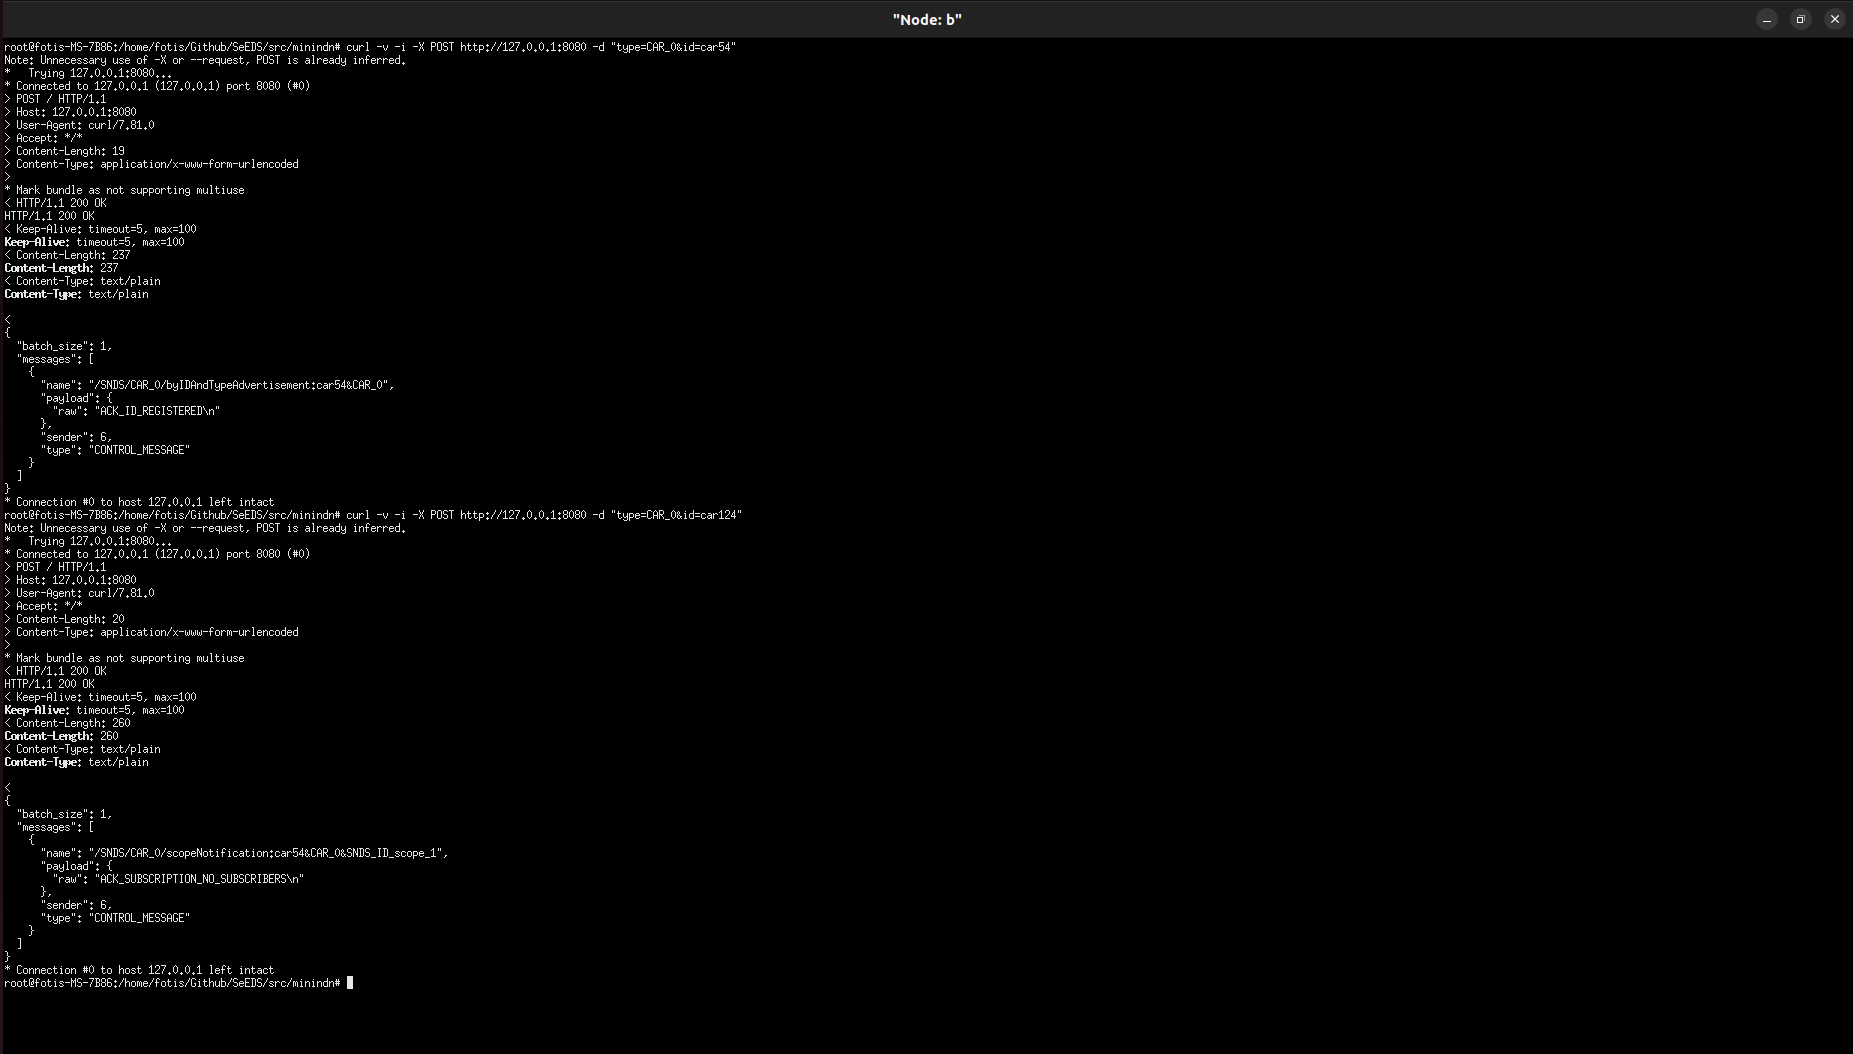
\includegraphics[width=1\linewidth]{images/post_to_registry_b_a.png}
    \caption{Posting the \textit{@ids=car54,car124} to the \textit{@type=CAR\_0} registry of A.}
    \label{fig:post_to_registry_b_a}
\end{figure}

\begin{figure}[H]
    \centering
    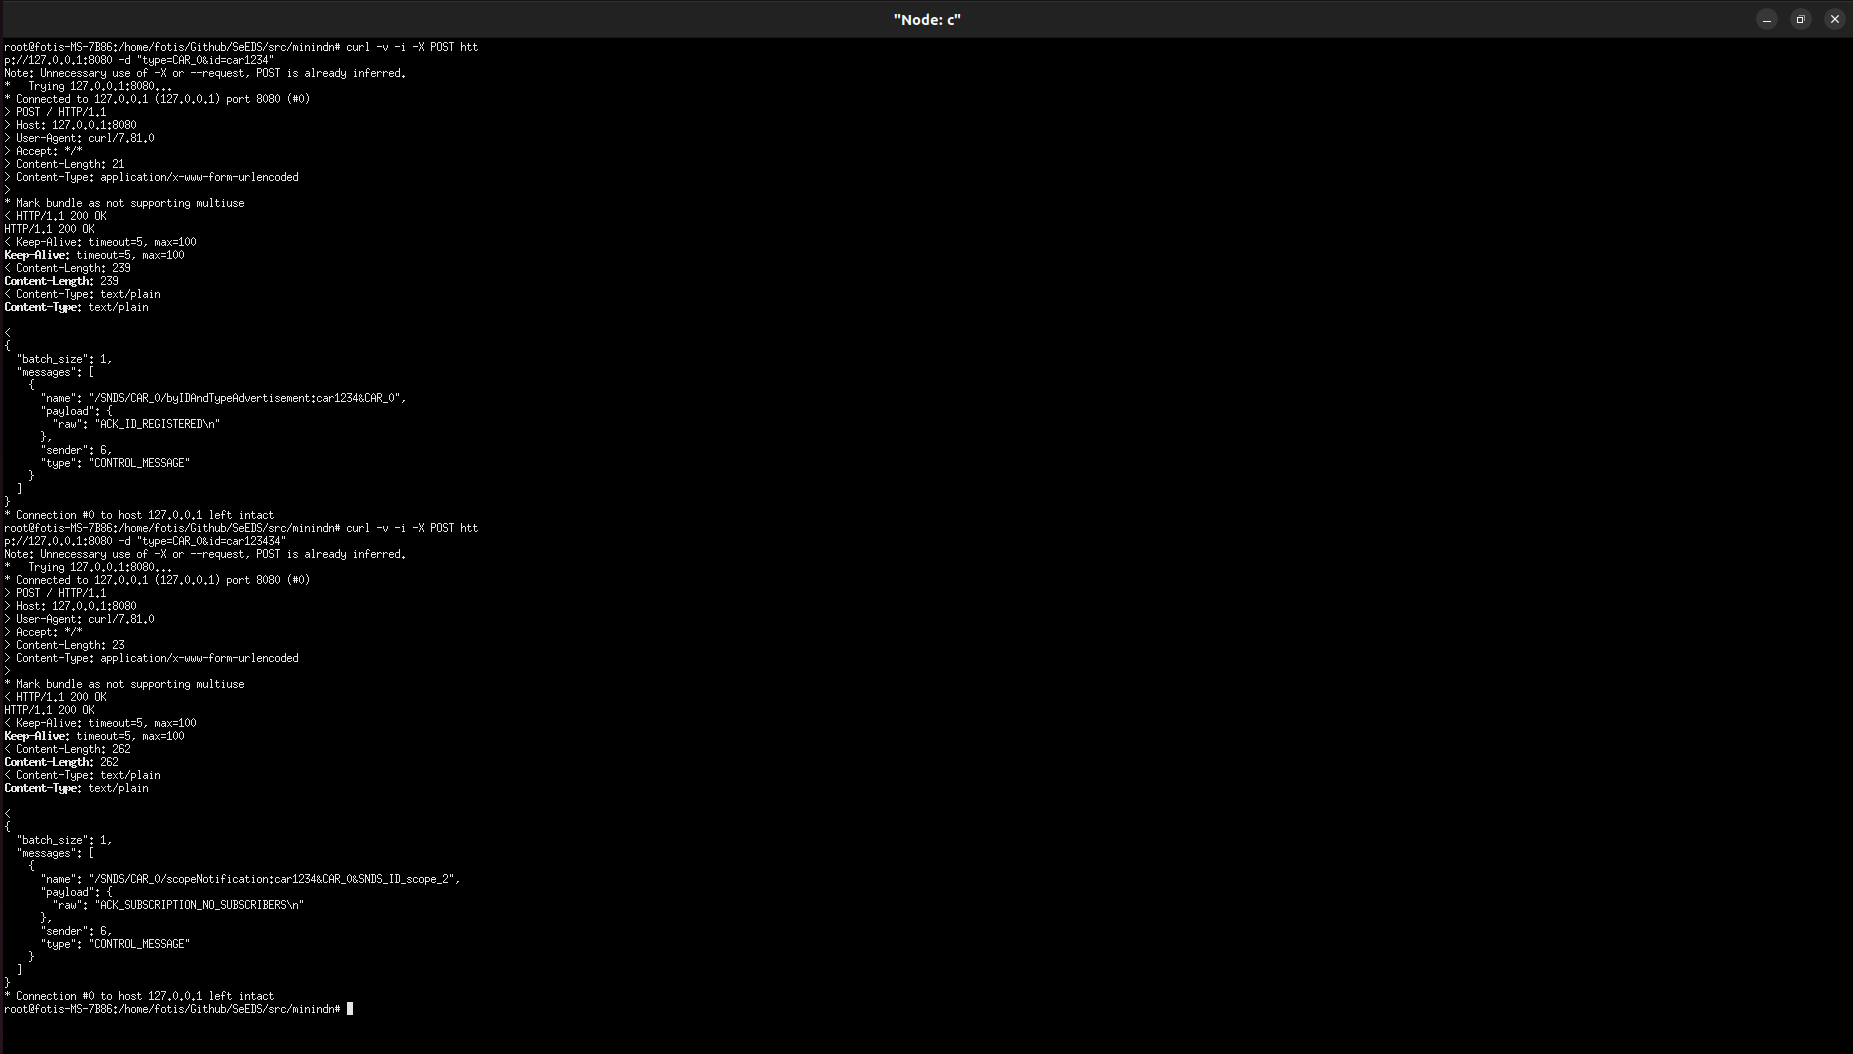
\includegraphics[width=1\linewidth]{images/post_to_registry_c_a.png}
    \caption{Posting the \textit{@ids=car123434,car1234} to the \textit{@type=CAR\_0} registry of A.}
    \label{fig:post_to_registry_c_a}
\end{figure}

Let's try to get A's registry through D: 

\begin{lstlisting}[language=log, caption={D after performing a GET by TYPE for CAR\_0},label={lst:get-by-type-d}]
[2025-09-25 00:16:25.868] [info] [Consumer] Sending actual Interest /SNDS/CAR_0_registry/getByType%3ACAR_0?CanBePrefix&Lifetime=6000
[2025-09-25 00:16:25.869] [info] [Consumer] Received Data with name: /SNDS/CAR_0_registry/getByType%3ACAR_0 in function onData
[2025-09-25 00:16:25.869] [info] [Consumer] Data packet payload: R car123434|car1234|car124|car54 in function onData
[2025-09-25 00:16:25.869] [info] [Consumer] Parsed interest: Prefix: SNDS, Name: CAR_0_registry, Command: getByType, Params: [CAR_0] in onData
[2025-09-25 00:16:25.869] [info] [Consumer] Received Registry File
[2025-09-25 00:16:25.869] [info] [Consumer] In Function: onData sending name CAR_0 to worker R	car123434|car1234|car124|car54
[2025-09-25 00:16:25.869] [info] [Worker] Received content: CAR_0
[2025-09-25 00:16:25.869] [info] [Consumer] Reading packet...
[2025-09-25 00:16:25.869] [info] [Worker] Received payload: R car123434|car1234|car124|car54
[2025-09-25 00:16:25.869] [info] [Worker] Received type: REGISTRY_PAYLOAD
[2025-09-25 00:16:25.869] [debug] [Worker] Consumer intra message...
[2025-09-25 00:16:25.869] [debug] [Worker] Number of IDs in payload: 4
[2025-09-25 00:16:25.869] [debug] [Worker] Reading ID #1 with size 9
[2025-09-25 00:16:25.869] [info] [Worker] Parsed ID #1: car123434
[2025-09-25 00:16:25.869] [debug] [Worker] Reading ID #2 with size 7
[2025-09-25 00:16:25.869] [info] [Worker] Parsed ID #2: car1234
[2025-09-25 00:16:25.869] [debug] [Worker] Reading ID #3 with size 6
[2025-09-25 00:16:25.869] [info] [Worker] Parsed ID #3: car124
[2025-09-25 00:16:25.869] [debug] [Worker] Reading ID #4 with size 5
[2025-09-25 00:16:25.869] [info] [Worker] Parsed ID #4: car54
[2025-09-25 00:16:25.869] [info] [Worker] Size of ids in registry file: 4
[2025-09-25 00:16:25.869] [debug] [Worker] Processing registry id: car123434
[2025-09-25 00:16:25.869] [info] [Worker] Pushing request to the consumer for id car123434
[2025-09-25 00:16:25.869] [debug] [Worker] Processing registry id: car1234
[2025-09-25 00:16:25.869] [info] [Worker] Pushing request to the consumer for id car1234
[2025-09-25 00:16:25.869] [debug] [Worker] Processing registry id: car124
[2025-09-25 00:16:25.869] [info] [Worker] Pushing request to the consumer for id car124
[2025-09-25 00:16:25.869] [debug] [Worker] Processing registry id: car54
[2025-09-25 00:16:25.869] [info] [Worker] Pushing request to the consumer for id car54
[2025-09-25 00:16:25.869] [debug] [Consumer] Extracted content from message: /SNDS/CAR_0/getByIDForType:car123434&CAR_0
[2025-09-25 00:16:25.869] [debug] [Consumer] Extracted content length from message: 42
[2025-09-25 00:16:25.869] [info] [Worker] Reading packet...
\end{lstlisting}


Reminder that each \hyperref[get_by_type_section]{GET by TYPE} request, becomes a \hyperref[get_by_id_section]{GET by ID} for each \textit{@ids} of the registry. D has successfully requested each \textit{@id} of the registry: 

\begin{lstlisting}[language=log, caption={D's log after receiving the registry payload, which are the \textit{@ids}, and performing a \emph{GET by ID} for each},label={lst:get-by-id-after-get-by-type-d}]
[2025-09-25 00:16:25.869] [debug] [Consumer] Extracted message type from message: GET_BY_ID_FOR_TYPE_REQUEST
[2025-09-25 00:16:25.869] [debug] [Consumer] Query.type: CAR_0
[2025-09-25 00:16:25.869] [debug] [Consumer] Query.id: car123434
[2025-09-25 00:16:25.869] [info] [Consumer] Created name /SNDS/CAR_0/temporalQuery:id%3Dcar123434&type%3DCAR_0&date%3D&count%3D&timeframe%3D&filters%3D
[2025-09-25 00:16:25.869] [info] [Consumer] Sending actual Interest /SNDS/CAR_0/temporalQuery%3Aid%3Dcar123434%26type%3DCAR_0%26date%3D%26count%3D%26timeframe%3D%26filters%3D?CanBePrefix&Lifetime=6000
[2025-09-25 00:16:25.871] [info] [Consumer] Received Data with name: /SNDS/CAR_0/temporalQuery%3Aid%3Dcar123434%26type%3DCAR_0%26date%3D%26count%3D%26timeframe%3D%26filters%3D in function onData
[2025-09-25 00:16:25.871] [info] [Consumer] Data packet payload: null in function onData
[2025-09-25 00:16:25.871] [info] [Consumer] Parsed interest: Prefix: SNDS, Name: CAR_0, Command: temporalQuery, Params: [id=car123434, type=CAR_0, date=, count=, timeframe=, filters=] in onData
[2025-09-25 00:16:25.871] [info] [Consumer] Temporal Query Reponse...
[2025-09-25 00:16:25.871] [error] [Consumer] No JSON start detected. First 32 bytes: 6e 75 6c 6c 
[2025-09-25 00:16:25.871] [info] [Consumer] Reading packet...
[2025-09-25 00:16:25.871] [debug] [Consumer] Extracted content from message: /SNDS/CAR_0/getByIDForType:car1234&CAR_0
[2025-09-25 00:16:25.871] [debug] [Consumer] Extracted content length from message: 40
[2025-09-25 00:16:25.871] [debug] [Consumer] Extracted message type from message: GET_BY_ID_FOR_TYPE_REQUEST
[2025-09-25 00:16:25.871] [debug] [Consumer] Query.type: CAR_0
[2025-09-25 00:16:25.871] [debug] [Consumer] Query.id: car1234
[2025-09-25 00:16:25.871] [info] [Consumer] Created name /SNDS/CAR_0/temporalQuery:id%3Dcar1234&type%3DCAR_0&date%3D&count%3D&timeframe%3D&filters%3D
[2025-09-25 00:16:25.871] [info] [Consumer] Sending actual Interest /SNDS/CAR_0/temporalQuery%3Aid%3Dcar1234%26type%3DCAR_0%26date%3D%26count%3D%26timeframe%3D%26filters%3D?CanBePrefix&Lifetime=6000
[2025-09-25 00:16:25.872] [info] [Consumer] Received Data with name: /SNDS/CAR_0/temporalQuery%3Aid%3Dcar1234%26type%3DCAR_0%26date%3D%26count%3D%26timeframe%3D%26filters%3D in function onData
[2025-09-25 00:16:25.872] [info] [Consumer] Data packet payload: null in function onData
[2025-09-25 00:16:25.872] [info] [Consumer] Parsed interest: Prefix: SNDS, Name: CAR_0, Command: temporalQuery, Params: [id=car1234, type=CAR_0, date=, count=, timeframe=, filters=] in onData
[2025-09-25 00:16:25.872] [info] [Consumer] Temporal Query Reponse...
[2025-09-25 00:16:25.872] [error] [Consumer] No JSON start detected. First 32 bytes: 6e 75 6c 6c 
[2025-09-25 00:16:25.872] [info] [Consumer] Reading packet...
[2025-09-25 00:16:25.872] [debug] [Consumer] Extracted content from message: /SNDS/CAR_0/getByIDForType:car124&CAR_0
[2025-09-25 00:16:25.872] [debug] [Consumer] Extracted content length from message: 39
[2025-09-25 00:16:25.872] [debug] [Consumer] Extracted message type from message: GET_BY_ID_FOR_TYPE_REQUEST
[2025-09-25 00:16:25.872] [debug] [Consumer] Query.type: CAR_0
[2025-09-25 00:16:25.872] [debug] [Consumer] Query.id: car124
[2025-09-25 00:16:25.872] [info] [Consumer] Created name /SNDS/CAR_0/temporalQuery:id%3Dcar124&type%3DCAR_0&date%3D&count%3D&timeframe%3D&filters%3D
[2025-09-25 00:16:25.872] [info] [Consumer] Sending actual Interest /SNDS/CAR_0/temporalQuery%3Aid%3Dcar124%26type%3DCAR_0%26date%3D%26count%3D%26timeframe%3D%26filters%3D?CanBePrefix&Lifetime=6000
[2025-09-25 00:16:25.874] [info] [Consumer] Received Data with name: /SNDS/CAR_0/temporalQuery%3Aid%3Dcar124%26type%3DCAR_0%26date%3D%26count%3D%26timeframe%3D%26filters%3D in function onData
[2025-09-25 00:16:25.874] [info] [Consumer] Data packet payload: null in function onData
[2025-09-25 00:16:25.874] [info] [Consumer] Parsed interest: Prefix: SNDS, Name: CAR_0, Command: temporalQuery, Params: [id=car124, type=CAR_0, date=, count=, timeframe=, filters=] in onData
[2025-09-25 00:16:25.874] [info] [Consumer] Temporal Query Reponse...
[2025-09-25 00:16:25.874] [error] [Consumer] No JSON start detected. First 32 bytes: 6e 75 6c 6c 
[2025-09-25 00:16:25.874] [info] [Consumer] Reading packet...
[2025-09-25 00:16:25.874] [debug] [Consumer] Extracted content from message: /SNDS/CAR_0/getByIDForType:car54&CAR_0
[2025-09-25 00:16:25.874] [debug] [Consumer] Extracted content length from message: 38
[2025-09-25 00:16:25.874] [debug] [Consumer] Extracted message type from message: GET_BY_ID_FOR_TYPE_REQUEST
[2025-09-25 00:16:25.874] [debug] [Consumer] Query.type: CAR_0
[2025-09-25 00:16:25.874] [debug] [Consumer] Query.id: car54
[2025-09-25 00:16:25.874] [info] [Consumer] Created name /SNDS/CAR_0/temporalQuery:id%3Dcar54&type%3DCAR_0&date%3D&count%3D&timeframe%3D&filters%3D
[2025-09-25 00:16:25.874] [info] [Consumer] Sending actual Interest /SNDS/CAR_0/temporalQuery%3Aid%3Dcar54%26type%3DCAR_0%26date%3D%26count%3D%26timeframe%3D%26filters%3D?CanBePrefix&Lifetime=6000
[2025-09-25 00:16:25.875] [info] [Consumer] Received Data with name: /SNDS/CAR_0/temporalQuery%3Aid%3Dcar54%26type%3DCAR_0%26date%3D%26count%3D%26timeframe%3D%26filters%3D in function onData
[2025-09-25 00:16:25.875] [info] [Consumer] Data packet payload: null in function onData
[2025-09-25 00:16:25.875] [info] [Consumer] Parsed interest: Prefix: SNDS, Name: CAR_0, Command: temporalQuery, Params: [id=car54, type=CAR_0, date=, count=, timeframe=, filters=] in onData
[2025-09-25 00:16:25.875] [info] [Consumer] Temporal Query Reponse...
[2025-09-25 00:16:25.875] [error] [Consumer] No JSON start detected. First 32 bytes: 6e 75 6c 6c 
[2025-09-25 00:16:25.875] [info] [Consumer] Reading packet...
\end{lstlisting}

The \textit{GET by TYPE} evaluation demonstrated the ability of SeEDS to retrieve data objects associated with a specific \textit{@type} across the distributed NDN network. By publishing multiple \textit{@ids} under the shared \textit{@type=CAR\_0} registry at node~A, other nodes, in this case node D, were able to discover and access the corresponding data through Interest packets constructed at the type level. This confirmed that the registry mechanism correctly advertises type scopes (e.g., \textit{/CAR\_0}) and propagates them throughout the network, enabling type-based content discovery.

The experiment verified that when a consumer issues a \textit{GET by TYPE} request, the SeEDS Service translates it into an NDN Interest targeting the appropriate registry scope. Node~A, acting as the producer, responds with the set of matching entries, allowing the consumer, in this case D, to perform a \emph{GET by ID} for each \textit{@id} (entry).

\subsection{Resilience (KPI 8)}

The experimental evaluation was conducted using MiniNDN. The primary objective of this experiment was to measure system resilience under partial failure conditions, with the specific target of demonstrating that recovery latency does not fall below 200 ms when 50\% of the data intermediary nodes fail.

\subsubsection{Topology}

The experimental evaluation was carried out on a seven-node star topology. In this configuration, node D functions as the central hub responsible for interconnecting all peripheral nodes through the Named Data Networking Forwarding Daemon (NFD). The peripheral nodes do not maintain direct links with one another; instead, every communication event must traverse the central hub. Consequently, all data exchanges and request forwarding operations are mediated by node D.

The nodes that will fail here are A,B,C which will be the Primary Nodes and the nodes that will be set up to be Secondary and remain alive will be E,F,G

\pagebreak

Here's a graph visualizing the topology:

\begin{figure}[H]
    \centering
    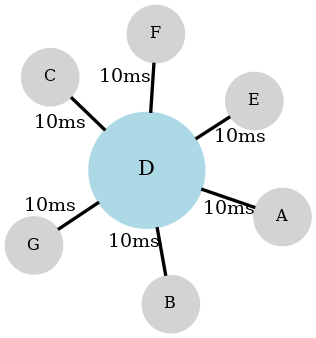
\includegraphics[width=0.5\linewidth]{images/star_topology.png}
    \caption{The above is a Star Topology with a central node ( hub ) interconnecting all the nodes in the network. The edge nodes in the circle F,E,C,G,B,A are the data nodes, responsible for publishing and getting data, while the hub acts just as an interconnector. The Primary Nodes A,B,C and the Secondary Nodes are E,F,G.}
    \label{fig:star-topology}
\end{figure}

Here's the config file inserted in MiniNDN:

\begin{lstlisting}[language=minindnconf, caption={The MiniNDN config for creating a star topology},label={lst:minindnconf-star-topology}]
[nodes]
a: _ nfd-log-level=DEBUG
b: _ nfd-log-level=DEBUG
c: _ nfd-log-level=DEBUG
d: _ nfd-log-level=DEBUG
e: _ nfd-log-level=DEBUG
f: _ nfd-log-level=DEBUG
g: _ nfd-log-level=DEBUG
[links]
d:a delay=10ms
a:d delay=10ms
d:b delay=10ms
b:d delay=10ms
c:d delay=10ms
d:c delay=10ms
d:e delay=10ms
e:d delay=10ms
d:f delay=10ms
f:d delay=10ms
d:g delay=10ms
g:d delay=10ms 
\end{lstlisting}

\subsubsection{Failure Injection}

To emulate node failures, we deliberately terminated half of the non-hub nodes during the experiment. This was achieved by applying a configurable timeout mechanism, after which the designated PRIMARY nodes were forced to stop their daemons and thus become unavailable. The remaining nodes (SECONDARY) continued to operate, monitoring their paired failing counterparts through the resilience poller.

\subsubsection{Data Replication}

Prior to node failures, data was actively published into the NDN network by all participating nodes. Each node contributed multiple data objects (e.g., key-value pairs of IDs and associated types) into the system, ensuring that the global dataset was replicated across the distributed instances running locally on each host. The publication mechanism guaranteed redundancy, such that information was not confined to a single point of failure.

\subsubsection{Failure Recovery and System Recovery Time}

Following the induced failures, retrieval operations were performed exclusively from the surviving SECONDARY nodes. By design, these nodes were configured to subscribe to content from their peers, ensuring that they could continue to respond to queries despite the absence of their PRIMARY counterparts. This allowed us to verify that replicated data remained accessible through alternative nodes.

Recovery was evaluated by analyzing the log files produced during the experiment. Each node continuously recorded system events with millisecond granularity. The recovery time metric was defined as the difference between two logged timestamps:

\begin{itemize}
    \item The timestamp recorded at the moment a PRIMARY node was declared failed, which corresponds to the daemon termination triggered by the timeout mechanism.
    \item The timestamp of the subsequent event when the paired SECONDARY node successfully published the final replicated data entry back into the NDN network.
    \item This difference represents the effective duration required for the system to detect the failure, promote the SECONDARY, and ensure that data availability was restored.
\end{itemize}

\subsubsection{Results of Failure Recovery}

Reminder that each node uses it's unique ID to make the following announcements:
\begin{lstlisting}[language=log,caption={Local announcements for each Node},label={lst:announcements-for-node-a}]
[2025-09-26 07:53:42.456] [info] [Producer] Announcing ID Scope name: SNDS/SNDS_ID_scope_id
[2025-09-26 07:53:42.456] [info] [Producer] Announcing name: SNDS/is_alive_id
[2025-09-26 07:53:42.456] [info] [Producer] Announcing name: SNDS/state_id
[2025-09-26 07:53:42.457] [info] [Producer] Announcing name: /SNDS/CAR_id
[2025-09-26 07:53:42.457] [info] [Producer] Announcing name: /SNDS/CAR_id_registry
[2025-09-26 07:53:42.458] [info] [Producer] Successfully registered prefix: /SNDS_id  

\end{lstlisting}

The \textit{ID} serves as a placeholder for each node’s unique identifier. The \emph{unique IDs} of each Node follow the alphabetical order and are zero-indexed. The Python script is configured to publish data to the node’s \textit{@type} and \textit{Subscriber} registries, as well as to publish the corresponding \textit{@ids} locally. This operation relies on each node’s \emph{unique node ID}. For instance, when publishing to node~A’s registry, which has a \emph{unique node ID} of~0, the data is published under the \textit{@type=CAR\_0} registry. Another example would be, that the \textit{@id=car0} should be published inside Node A or the \textit{@id=car1} should be published inside Node B. This procedure is repeated for all \emph{Nodes}, ensuring that each node maintains and announces its own unique data within the network. Recall that the \emph{Primary Nodes} are A,B,C so we should expect the \emph{Secondary Nodes} E,F,G to contain the data of the \emph{Primaries} once they fail.


\textbf{Inside node A} we must see \textit{@id=car0} get announced successfully:

\begin{lstlisting}[language=log,caption={Publish \textit{@id=car0}},label={lst:local-publish-inside-a}]
[2025-09-26 10:01:07.876] [info] [HTTPServer] Received POST request for / with body id=car0
[2025-09-26 10:01:07.876] [info] [HTTPServer] Received POST request from 127.0.0.1
Message: {id=car0}
Type: BY_ID_ADVERTISEMENT
Sender: HTTP_SRV
Payload: 
HTTP Type: HTTP_POST
Params:
id = car0
[2025-09-26 10:01:07.876] [debug] [HTTPServer] Writing message from POST request to service queue...
Message: {id=car0}
Type: BY_ID_ADVERTISEMENT
Sender: HTTP_SRV
Payload: 
HTTP Type: HTTP_POST
Params:
id = car0

[2025-09-26 10:01:07.876] [debug] [DigitalTwin] Extracted content from message {id=car0}
[2025-09-26 10:01:07.876] [debug] [DigitalTwin] Extracted content length from message 9
[2025-09-26 10:01:07.876] [debug] [DigitalTwin] Extracted type from message: BY_ID_ADVERTISEMENT
[2025-09-26 10:01:07.876] [info] [DigitalTwin] Received by ID get request...
[2025-09-26 10:01:07.876] [debug] [DigitalTwin] Pushed ID car0 to the announced IDs vector...
[2025-09-26 10:01:07.876] [debug] [DigitalTwin] Extracted id Scope from message SNDS_ID_scope_0
Message: /SNDS/car0/postID:car0
Type: BY_ID_ADVERTISEMENT
Sender: DIGITAL_TWIN
Payload: 
HTTP Type: HTTP_EMPTY
Params:
[2025-09-26 10:01:07.876] [info] [DigitalTwin] Pushing byID advertisement to the Producer...
Message: /SNDS/car0/postID:car0
Type: BY_ID_ADVERTISEMENT
Sender: DIGITAL_TWIN
Payload: 
HTTP Type: HTTP_EMPTY
Params:

[2025-09-26 10:01:07.876] [debug] [DigitalTwin] Sleeping 2000 ms before sending scope advertisement...
[2025-09-26 10:01:07.880] [info] [Producer] Received interest in function: onInterest, name: /SNDS/state_0/getResilienceMeta%3A
[2025-09-26 10:01:07.880] [info] [Producer] Parsed interest: Prefix: SNDS, Name: state_0, Command: getResilienceMeta, Params: []
[2025-09-26 10:01:07.881] [info] [Producer] Received interest in function: onInterest, name: /SNDS/is_alive_0/getResilienceIsAlive%3A17432869098159683528
[2025-09-26 10:01:07.882] [info] [Producer] Parsed interest: Prefix: SNDS, Name: is_alive_0, Command: getResilienceIsAlive, Params: [17432869098159683528]
[2025-09-26 10:01:07.882] [debug] [Producer] Sending data to the NDN…
[2025-09-26 10:01:07.902] [info] [Producer] Received interest in function: onInterest, name: /SNDS/is_alive_0/getResilienceIsAlive%3A11341762269107256235
[2025-09-26 10:01:07.902] [info] [Producer] Parsed interest: Prefix: SNDS, Name: is_alive_0, Command: getResilienceIsAlive, Params: [11341762269107256235]
[2025-09-26 10:01:07.902] [debug] [Producer] Sending data to the NDN…
[2025-09-26 10:01:07.920] [info] [Producer] Received interest in function: onInterest, name: /SNDS/state_0/getResilienceMeta%3A
[2025-09-26 10:01:07.920] [info] [Producer] Parsed interest: Prefix: SNDS, Name: state_0, Command: getResilienceMeta, Params: []
[2025-09-26 10:01:07.922] [info] [Producer] Received interest in function: onInterest, name: /SNDS/is_alive_0/getResilienceIsAlive%3A7264770695334591861
[2025-09-26 10:01:07.922] [info] [Producer] Parsed interest: Prefix: SNDS, Name: is_alive_0, Command: getResilienceIsAlive, Params: [7264770695334591861]
[2025-09-26 10:01:07.922] [debug] [Producer] Sending data to the NDN…
[2025-09-26 10:01:07.942] [info] [Producer] Received interest in function: onInterest, name: /SNDS/is_alive_0/getResilienceIsAlive%3A10537152589682238699
[2025-09-26 10:01:07.942] [info] [Producer] Parsed interest: Prefix: SNDS, Name: is_alive_0, Command: getResilienceIsAlive, Params: [10537152589682238699]
[2025-09-26 10:01:07.942] [debug] [Producer] Sending data to the NDN…
[2025-09-26 10:01:07.960] [info] [Producer] Received interest in function: onInterest, name: /SNDS/state_0/getResilienceMeta%3A
[2025-09-26 10:01:07.960] [info] [Producer] Parsed interest: Prefix: SNDS, Name: state_0, Command: getResilienceMeta, Params: []
[2025-09-26 10:01:07.962] [info] [Producer] Received interest in function: onInterest, name: /SNDS/is_alive_0/getResilienceIsAlive%3A12718435922522655948
[2025-09-26 10:01:07.962] [info] [Producer] Parsed interest: Prefix: SNDS, Name: is_alive_0, Command: getResilienceIsAlive, Params: [12718435922522655948]
[2025-09-26 10:01:07.962] [debug] [Producer] Sending data to the NDN…
Message: /SNDS/car0/postID:car0
Type: BY_ID_ADVERTISEMENT
Sender: DIGITAL_TWIN
Payload: 
HTTP Type: HTTP_EMPTY
Params:
[2025-09-26 10:01:07.971] [info] [Producer] Got new ID advertisement request...
Message: /SNDS/car0/postID:car0
Type: BY_ID_ADVERTISEMENT
Sender: DIGITAL_TWIN
Payload: 
HTTP Type: HTTP_EMPTY
Params:

[2025-09-26 10:01:07.971] [debug] [Producer] Parsed interest Prefix: SNDS, Name: car0, Command: postID, Params: [car0] from string
[2025-09-26 10:01:07.971] [info] [Producer] Announcing name: /SNDS/car0
\end{lstlisting}

We can see in the above that Node A successfully published \textit{@id=car0} to the NDN network.


\textbf{Inside Node B} we should see \textit{@id=car1} get announced successfully: 


\begin{lstlisting}[language=log, caption={}, label={lst:announcements-for-node-b}]
[2025-09-26 10:01:19.920] [info] [HTTPServer] Received POST request for / with body id=car1
[2025-09-26 10:01:19.920] [info] [HTTPServer] Received POST request from 127.0.0.1
Message: {id=car1}
Type: BY_ID_ADVERTISEMENT
Sender: HTTP_SRV
Payload: 
HTTP Type: HTTP_POST
Params:
id = car1
[2025-09-26 10:01:19.920] [debug] [HTTPServer] Writing message from POST request to service queue...
Message: {id=car1}
Type: BY_ID_ADVERTISEMENT
Sender: HTTP_SRV
Payload: 
HTTP Type: HTTP_POST
Params:
id = car1

[2025-09-26 10:01:19.920] [debug] [DigitalTwin] Extracted content from message {id=car1}
[2025-09-26 10:01:19.920] [debug] [DigitalTwin] Extracted content length from message 9
[2025-09-26 10:01:19.920] [debug] [DigitalTwin] Extracted type from message: BY_ID_ADVERTISEMENT
[2025-09-26 10:01:19.920] [info] [DigitalTwin] Received by ID get request...
[2025-09-26 10:01:19.920] [debug] [DigitalTwin] Pushed ID car1 to the announced IDs vector...
[2025-09-26 10:01:19.920] [debug] [DigitalTwin] Extracted id Scope from message SNDS_ID_scope_5
Message: /SNDS/car1/postID:car1
Type: BY_ID_ADVERTISEMENT
Sender: DIGITAL_TWIN
Payload: 
HTTP Type: HTTP_EMPTY
Params:
[2025-09-26 10:01:19.920] [info] [DigitalTwin] Pushing byID advertisement to the Producer...
Message: /SNDS/car1/postID:car1
Type: BY_ID_ADVERTISEMENT
Sender: DIGITAL_TWIN
Payload: 
HTTP Type: HTTP_EMPTY
Params:

[2025-09-26 10:01:19.920] [debug] [DigitalTwin] Sleeping 2000 ms before sending scope advertisement...
Message: /SNDS/car1/postID:car1
Type: BY_ID_ADVERTISEMENT
Sender: DIGITAL_TWIN
Payload: 
HTTP Type: HTTP_EMPTY
Params:
[2025-09-26 10:01:19.921] [info] [Producer] Got new ID advertisement request...
Message: /SNDS/car1/postID:car1
Type: BY_ID_ADVERTISEMENT
Sender: DIGITAL_TWIN
Payload: 
HTTP Type: HTTP_EMPTY
Params:

[2025-09-26 10:01:19.921] [debug] [Producer] Parsed interest Prefix: SNDS, Name: car1, Command: postID, Params: [car1] from string
[2025-09-26 10:01:19.921] [info] [Producer] Announcing name: /SNDS/car1
\end{lstlisting}

Now let's check whether the \emph{Secondary Nodes} can actually recover. Here's the timestamp when the \emph{A Node} shutdown: 

\begin{lstlisting}[language=log, caption={A's timeout timestamp}, label={lst:a-timeout-timestamp}]
[TIMEOUT] 2025-09-26 10:03:08.446 a: daemon exceeded timeout 
\end{lstlisting}

Node E's logs which is set up to be the \emph{Secondary Node} of A:

\begin{lstlisting}[language=log, caption={E's recovery logs}, label={lst:e-recovery-logs}]
[2025-09-26 10:03:08.456] [warning] [Producer] [resilience-ipc] promotion to PRIMARY (reason=alive-missed, misses=1)
[2025-09-26 10:03:08.456] [info] [Producer] [resilience] mutate → ver=6 hash=73f0555c38af9c19ece369fcb898abc0
[2025-09-26 10:03:08.456] [debug] [Producer] [resilience] history versions: 0(37a6259c) 1(c76727ce) 2(04168ec0) 3(b4d35eeb) 4(e9df653a) 5(0ef09630) 6(73f0555c) 
[2025-09-26 10:03:08.456] [debug] [Producer] [resilience] ops from v5 → v6:
[
  {
    "op": "replace",
    "path": "/resilience/reason",
    "value": "alive-missed"
  },
  {
    "op": "replace",
    "path": "/resilience/role",
    "value": "primary"
  },
  {
    "op": "replace",
    "path": "/resilience/since",
    "value": "2025-09-26T07:03:08Z"
  },
  {
    "op": "add",
    "path": "/resilience/misses",
    "value": 1
  }
]
[2025-09-26 10:03:08.456] [warning] [Producer] [resilience-ipc] stop requested; will be joined from main loop
[2025-09-26 10:03:08.522] [warning] [Producer] [resilience] applying promotion side-effects on main loop
[2025-09-26 10:03:08.522] [debug] [Producer] [overlay] merge: applying json_patch_against_base (ops=7)
[2025-09-26 10:03:08.522] [debug] [Producer] [resilience] assign → ver=7 hash=19f8dbf49001bae4f664a330312d42a9
[2025-09-26 10:03:08.522] [debug] [Producer] [overlay] SQUASH → base version 6→7  hash 73f0555c38af9c19ece369fcb898abc0→19f8dbf49001bae4f664a330312d42a9  overlay ver=16 hash=994121709bfc030ff093864add91033d
[2025-09-26 10:03:08.522] [debug] [Producer] [overlay] CLEARED
[2025-09-26 10:03:08.523] [debug] [Producer] [promotion] rebuilt containers from store:
[2025-09-26 10:03:08.523] [debug] [Producer]   type_registry[CAR_0] = [car10 ]
[2025-09-26 10:03:08.523] [debug] [Producer]   type_registry[CAR_4] = [car14 ]
[2025-09-26 10:03:08.523] [debug] [Producer]   subscribed_nodes_for_type[CAR_0] = [SNDS_ID_scope_6 ]
[2025-09-26 10:03:08.523] [debug] [Producer]   subscribed_nodes_for_type[CAR_4] = [SNDS_ID_scope_3 ]
[2025-09-26 10:03:08.523] [debug] [Producer]   announcements = [/SNDS/SNDS_ID_scope_4 /SNDS/is_alive_4 /SNDS/state_4 /SNDS/CAR_4_registry /SNDS/CAR_4 /SNDS/car4 /SNDS_0 /SNDS/car0 /SNDS/CAR_0 /SNDS/CAR_0_registry /SNDS/is_alive_0 /SNDS/SNDS_ID_scope_0 /SNDS_4 /SNDS/state_0 ]
[2025-09-26 10:03:08.523] [info] [Producer] [promotion] summary: types=2 ids=2 subs(byId)=0 subs(byType)=2 announced=14
[2025-09-26 10:03:08.523] [info] [Producer] [promotion] (re)announcing /SNDS/SNDS_ID_scope_4
[2025-09-26 10:03:08.523] [info] [Producer] [promotion] (re)announcing /SNDS/is_alive_4
[2025-09-26 10:03:08.523] [info] [Producer] [promotion] (re)announcing /SNDS/state_4
[2025-09-26 10:03:08.523] [info] [Producer] [promotion] (re)announcing /SNDS/CAR_4_registry
[2025-09-26 10:03:08.523] [info] [Producer] [promotion] (re)announcing /SNDS/CAR_4
[2025-09-26 10:03:08.523] [info] [Producer] [promotion] (re)announcing /SNDS/car4
[2025-09-26 10:03:08.524] [info] [Producer] [promotion] (re)announcing /SNDS_0
[2025-09-26 10:03:08.524] [info] [Producer] [promotion] (re)announcing /SNDS/car0
[2025-09-26 10:03:08.524] [info] [Producer] [promotion] (re)announcing /SNDS/CAR_0
[2025-09-26 10:03:08.524] [info] [Producer] [promotion] (re)announcing /SNDS/CAR_0_registry
[2025-09-26 10:03:08.524] [info] [Producer] [promotion] (re)announcing /SNDS/is_alive_0
[2025-09-26 10:03:08.524] [info] [Producer] [promotion] (re)announcing /SNDS/SNDS_ID_scope_0
[2025-09-26 10:03:08.524] [info] [Producer] [promotion] (re)announcing /SNDS_4
[2025-09-26 10:03:08.525] [info] [Producer] [promotion] (re)announcing /SNDS/state_0
[2025-09-26 10:03:08.525] [info] [Producer] Getting from IP: 10.0.0.26 and port: 10000
[2025-09-26 10:03:08.525] [debug] [Producer] HTTP GET /state?type=CAR_0
[2025-09-26 10:03:08.527] [info] [Producer] [resilience] mutate → ver=8 hash=85a5cbdd3d895ce5212470a8dfe17f55
[2025-09-26 10:03:08.527] [debug] [Producer] [resilience] history versions: 0(37a6259c) 1(c76727ce) 2(04168ec0) 3(b4d35eeb) 4(e9df653a) 5(0ef09630) 6(73f0555c) 7(19f8dbf4) 8(85a5cbdd) 
[2025-09-26 10:03:08.527] [debug] [Producer] [resilience] ops from v7 → v8:
[
  {
    "op": "replace",
    "path": "/broker/collections/CAR_0/lastSeen",
    "value": "2025-09-26T07:03:08Z"
  }
]
[2025-09-26 10:03:08.527] [info] [Producer] Getting from IP: 10.0.0.26 and port: 10000
[2025-09-26 10:03:08.527] [debug] [Producer] HTTP GET /state?type=CAR_4
[2025-09-26 10:03:08.528] [info] [Producer] [resilience] mutate → ver=9 hash=71624b465ef5120729971953ad41ec36
[2025-09-26 10:03:08.529] [debug] [Producer] [resilience] history versions: 0(37a6259c) 1(c76727ce) 2(04168ec0) 3(b4d35eeb) 4(e9df653a) 5(0ef09630) 6(73f0555c) 7(19f8dbf4) 8(85a5cbdd) 9(71624b46) 
[2025-09-26 10:03:08.529] [debug] [Producer] [resilience] ops from v8 → v9:
[
  {
    "op": "add",
    "path": "/broker/collections/CAR_4",
    "value": {
      "algo": "SHA-256",
      "count": 0,
      "hash": "e3b0c44298fc1c149afbf4c8996fb92427ae41e4649b934ca495991b7852b855",
      "lastSeen": "2025-09-26T07:03:08Z"
    }
  }
]
[2025-09-26 10:03:08.530] [info] [Producer] Successfully registered prefix: /SNDS/SNDS_ID_scope_4
[2025-09-26 10:03:08.530] [info] [Producer] Successfully registered prefix: /SNDS/is_alive_4
[2025-09-26 10:03:08.530] [info] [Producer] Successfully registered prefix: /SNDS/state_4
[2025-09-26 10:03:08.530] [info] [Producer] Successfully registered prefix: /SNDS/CAR_4_registry
[2025-09-26 10:03:08.532] [info] [Producer] Successfully registered prefix: /SNDS/CAR_4
[2025-09-26 10:03:08.532] [info] [Producer] Successfully registered prefix: /SNDS/car4
[2025-09-26 10:03:08.533] [info] [Producer] Successfully registered prefix: /SNDS_0
[2025-09-26 10:03:08.533] [info] [Producer] Successfully registered prefix: /SNDS/car0
[2025-09-26 10:03:08.533] [info] [Producer] Successfully registered prefix: /SNDS/CAR_0
[2025-09-26 10:03:08.533] [info] [Producer] Successfully registered prefix: /SNDS/CAR_0_registry
[2025-09-26 10:03:08.533] [info] [Producer] Successfully registered prefix: /SNDS/is_alive_0
[2025-09-26 10:03:08.533] [info] [Producer] Successfully registered prefix: /SNDS/SNDS_ID_scope_0
[2025-09-26 10:03:08.533] [info] [Producer] Successfully registered prefix: /SNDS_4
[2025-09-26 10:03:08.533] [info] [Producer] Successfully registered prefix: /SNDS/state_0 
\end{lstlisting}

We can see that the failure of Node A happened at \textbf{2025-09-26 10:03:08.446} and the Secondary Node published the last data at \textbf{2025-09-26 10:03:08.533}. This means that the system recovered in \emph{87ms}. This is to be expected, because the data is continuously replicated in our system and it is essentially ready to be published once the Primary Node fails.

Let's see now if the data of A, which now are essentially the data of E, are retrievable through the network. Let's ask for the data through G, which is the \textit{@id=car0}:

\begin{figure}][H]
    \centering
    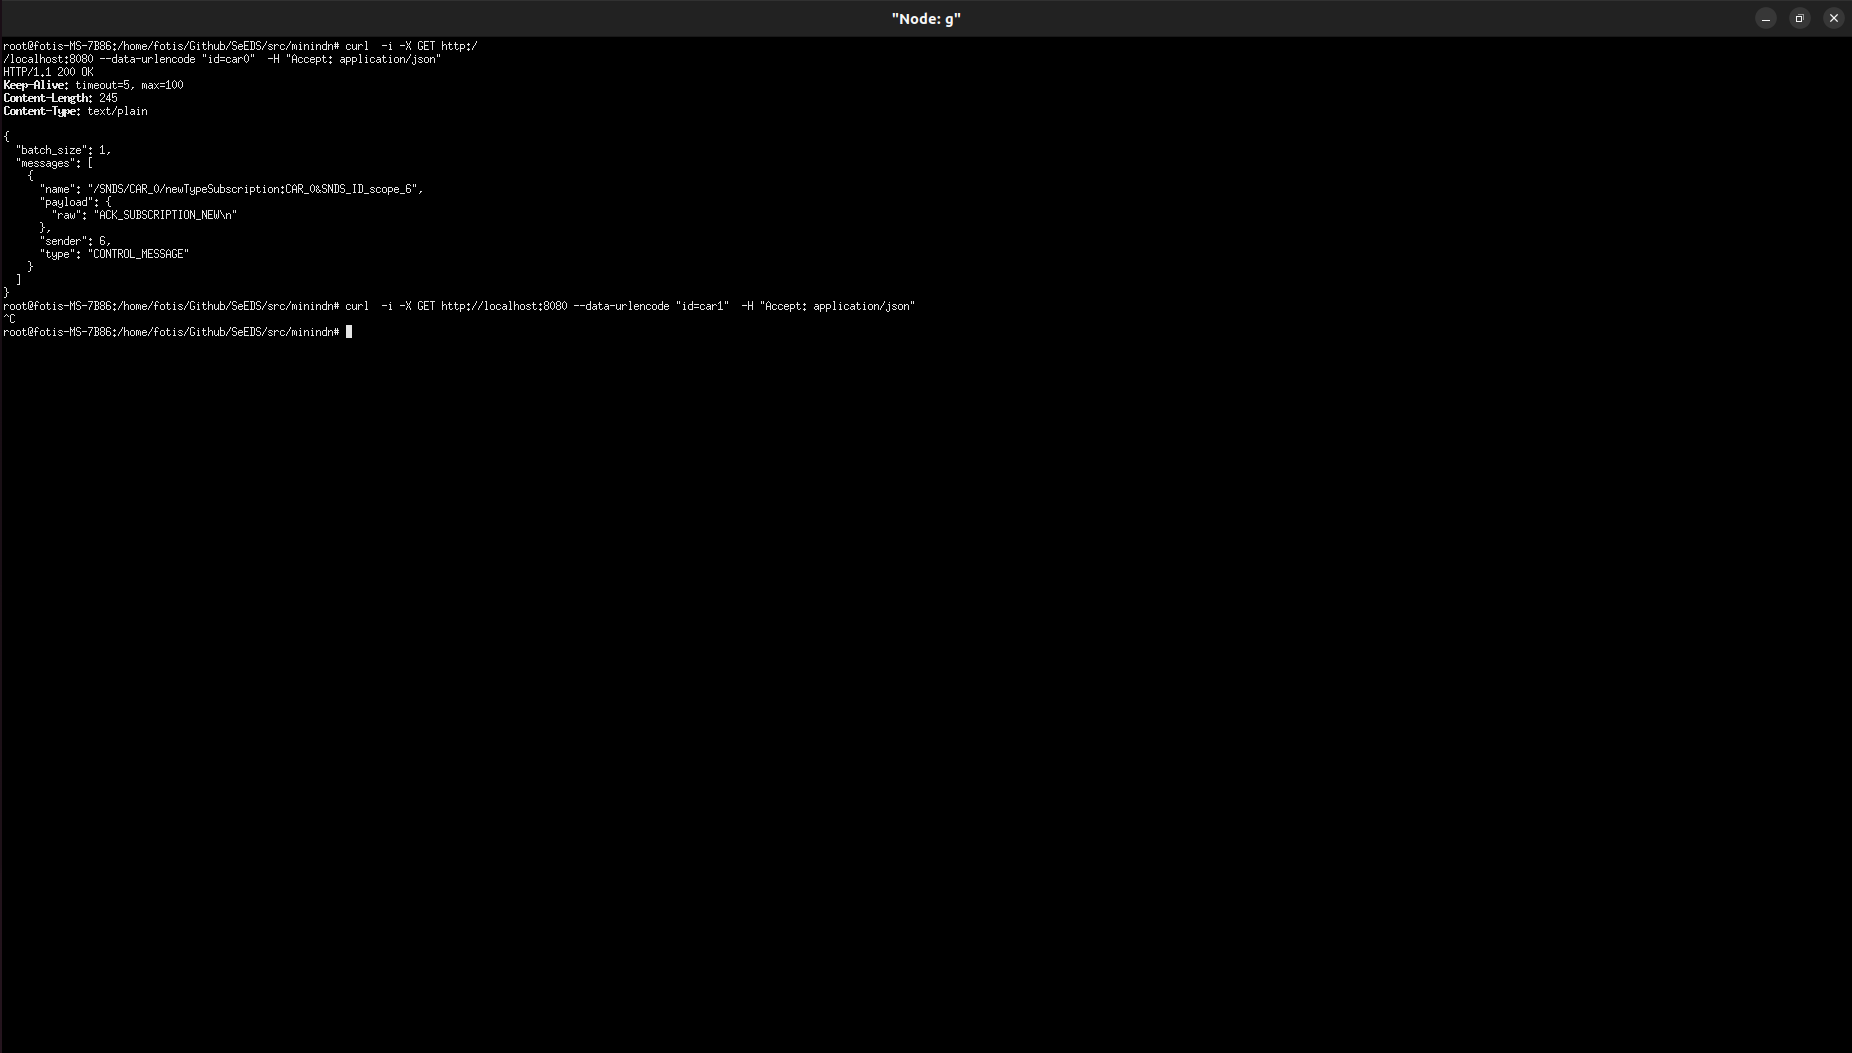
\includegraphics[width=0.5\linewidth]{images/after_failure_through_g.png}
    \caption{Request \textit{@id=car0} and \textit{@id=car1} through G.}
    \label{fig:placeholder}
\end{figure}

Let's check E's logs, which now provides the data of A:

\begin{lstlisting}[language=log, caption={E's logs after becoming the provider of A's data}, label={lst:e-after-failure-producer}]
[2025-09-26 10:22:14.393] [info] [Producer] Received interest in function: onInterest, name: /SNDS/car0/temporalQuery%3Aid%3Dcar0%26type%3D%26date%3D%26count%3D%26timeframe%3D%26filters%3D
[2025-09-26 10:22:14.394] [info] [Producer] Parsed interest: Prefix: SNDS, Name: car0, Command: temporalQuery, Params: [id=car0, type=, date=, count=, timeframe=, filters=]
[2025-09-26 10:22:14.394] [debug] [Producer] Created interest response: /SNDS/car0/temporalQuery%3Aid%3Dcar0%26type%3D%26date%3D%26count%3D%26timeframe%3D%26filters%3D in: process_temporal_query_interest
[2025-09-26 10:22:14.394] [debug] [Producer] TemporalQuery → id: car0, date: , type: , timeframe: , count: , filters: 
[2025-09-26 10:22:14.394] [debug] [Producer] Requesting to endpoint: /temporal-query?id=car0&type=&count=&date=&timeframe=&filters=
[2025-09-26 10:22:14.395] [info] [Producer] Successfully queried /temporal-query
[2025-09-26 10:22:14.395] [debug] [Producer] Sending data to the NDN…
\end{lstlisting}

Let's check G's logs, which requests the data of A:

\begin{lstlisting}[language=log, caption={G performs the request to retrieve ex A's data, which are now provided through E}, label={lst:g-get-data-from-e}]
[2025-09-26 10:22:14.393] [info] [HTTPServer] Received GET request for / with body id=car0
[2025-09-26 10:22:14.393] [info] [HTTPServer] Received GET request for / with target /
[2025-09-26 10:22:14.393] [info] [HTTPServer] Received GET request from 127.0.0.1
Message: {id=car0}
Type: GET_BY_ID_REQUEST
Sender: HTTP_SRV
Payload: 
HTTP Type: HTTP_GET
Params:
id = car0
[2025-09-26 10:22:14.393] [debug] [HTTPServer] Writing message from GET request to service queue...
Message: {id=car0}
Type: GET_BY_ID_REQUEST
Sender: HTTP_SRV
Payload: 
HTTP Type: HTTP_GET
Params:
id = car0

[2025-09-26 10:22:14.393] [info] [Worker] Received content: {id=car0}
[2025-09-26 10:22:14.393] [info] [Worker] Received payload: 
[2025-09-26 10:22:14.393] [info] [Worker] Received type: GET_BY_ID_REQUEST
[2025-09-26 10:22:14.393] [debug] [Worker] Server intra message...
Message: BATCH
Type: GENERIC
Sender: WORKER
Payload: {
  "batch_size": 1,
  "messages": [
    {
      "name": "/SNDS/CAR_0/newTypeSubscription:CAR_0&SNDS_ID_scope_6",
      "payload": {
        "raw": "ACK_SUBSCRIPTION_NEW\n"
      },
      "sender": 6,
      "type": "CONTROL_MESSAGE"
    }
  ]
}

HTTP Type: HTTP_EMPTY
Params:
[2025-09-26 10:22:14.393] [info] [HTTPServer] Read Message from queue:
Message: BATCH
Type: GENERIC
Sender: WORKER
Payload: {
  "batch_size": 1,
  "messages": [
    {
      "name": "/SNDS/CAR_0/newTypeSubscription:CAR_0&SNDS_ID_scope_6",
      "payload": {
        "raw": "ACK_SUBSCRIPTION_NEW\n"
      },
      "sender": 6,
      "type": "CONTROL_MESSAGE"
    }
  ]
}

HTTP Type: HTTP_EMPTY
Params:

[2025-09-26 10:22:14.393] [info] [Worker] Inserted ID: car0 into set. Pushing regular getByID request for ID: car0
[2025-09-26 10:22:14.393] [info] [Worker] Reading packet...
[2025-09-26 10:22:14.393] [debug] [Consumer] Extracted content from message: /SNDS/car0/getByID:car0
[2025-09-26 10:22:14.393] [debug] [Consumer] Extracted content length from message: 23
[2025-09-26 10:22:14.393] [debug] [Consumer] Extracted message type from message: GET_BY_ID_REQUEST
[2025-09-26 10:22:14.393] [debug] [Consumer] Query.type: 
[2025-09-26 10:22:14.393] [debug] [Consumer] Query.id: car0
[2025-09-26 10:22:14.393] [info] [Consumer] Created name /SNDS/car0/temporalQuery:id%3Dcar0&type%3D&date%3D&count%3D&timeframe%3D&filters%3D
[2025-09-26 10:22:14.393] [info] [Consumer] Sending actual Interest /SNDS/car0/temporalQuery%3Aid%3Dcar0%26type%3D%26date%3D%26count%3D%26timeframe%3D%26filters%3D?CanBePrefix&Lifetime=6000
[2025-09-26 10:22:14.396] [info] [Consumer] Received Data with name: /SNDS/car0/temporalQuery%3Aid%3Dcar0%26type%3D%26date%3D%26count%3D%26timeframe%3D%26filters%3D in function onData
[2025-09-26 10:22:14.396] [info] [Consumer] Data packet payload: [
  {
    "": {
      "_id": "car0",
      "id": "car0",
      "timestamp": {
        "$date": 1758870068072
      },
      "type": "GENERIC"
    }
  }
] in function onData
[2025-09-26 10:22:14.396] [info] [Consumer] Parsed interest: Prefix: SNDS, Name: car0, Command: temporalQuery, Params: [id=car0, type=, date=, count=, timeframe=, filters=] in onData
[2025-09-26 10:22:14.396] [info] [Consumer] Temporal Query Reponse...
[2025-09-26 10:22:14.396] [debug] [Consumer] Removed extra characters from payload (first 32 bytes hex): 5b 0a 20 20 7b 0a 20 20 20 20 22 22 3a 20 7b 0a 20 20 20 20 20 20 22 5f 69 64 22 3a 20 22 63 61 
[2025-09-26 10:22:14.396] [debug] [Consumer] Candidate JSON slice:
[
  {
    "": {
      "_id": "car0",
      "id": "car0",
      "timestamp": {
        "$date": 1758870068072
      },
      "type": "GENERIC"
    }
  }
]
[2025-09-26 10:22:14.396] [debug] [Consumer] Sanitized payload to:
[
  {
    "": {
      "_id": "car0",
      "id": "car0",
      "timestamp": {
        "$date": 1758870068072
      },
      "type": "GENERIC"
    }
  }
]    
\end{lstlisting}

We can see that G got a response back with data, after requesting it from E.

Let's also check B's logs, which is another Primary Node:

\begin{lstlisting}[language=log, caption={Timeout timestamp of Node B}, label={lst:timeout-b}]
[TIMEOUT] 2025-09-26 10:03:11.493 b: daemon exceeded timeout
\end{lstlisting}

Let's check F's logs, which is the Secondary Node of B:

\begin{lstlisting}[language=log, caption={Logs of Node F after providing the data of Node B}, label={lst:f-becoming-primary}]
[2025-09-26 10:03:11.496] [warning] [Producer] [resilience-ipc] promotion to PRIMARY (reason=alive-missed, misses=1)
[2025-09-26 10:03:11.496] [info] [Producer] [resilience] mutate → ver=6 hash=ac41eea00ae8385b88550b5d064cee98
[2025-09-26 10:03:11.496] [debug] [Producer] [resilience] history versions: 0(37a6259c) 1(3b6ede70) 2(b4b2de78) 3(050d6435) 4(20c5c4af) 5(7ee82c13) 6(ac41eea0) 
[2025-09-26 10:03:11.496] [debug] [Producer] [resilience] ops from v5 → v6:
[
  {
    "op": "replace",
    "path": "/resilience/reason",
    "value": "alive-missed"
  },
  {
    "op": "replace",
    "path": "/resilience/role",
    "value": "primary"
  },
  {
    "op": "replace",
    "path": "/resilience/since",
    "value": "2025-09-26T07:03:11Z"
  },
  {
    "op": "add",
    "path": "/resilience/misses",
    "value": 1
  }
]
[2025-09-26 10:03:11.496] [warning] [Producer] [resilience-ipc] stop requested; will be joined from main loop
[2025-09-26 10:03:11.530] [warning] [Producer] [resilience] applying promotion side-effects on main loop
[2025-09-26 10:03:11.530] [debug] [Producer] [overlay] merge: applying json_patch_against_base (ops=7)
[2025-09-26 10:03:11.530] [debug] [Producer] [resilience] assign → ver=7 hash=9b408c51324d2bb669672017a28994e2
[2025-09-26 10:03:11.530] [debug] [Producer] [overlay] SQUASH → base version 6→7  hash ac41eea00ae8385b88550b5d064cee98→9b408c51324d2bb669672017a28994e2  overlay ver=16 hash=59d0966e24c8873e2ec151dfd7a8b395
[2025-09-26 10:03:11.530] [debug] [Producer] [overlay] CLEARED
[2025-09-26 10:03:11.530] [debug] [Producer] [promotion] rebuilt containers from store:
[2025-09-26 10:03:11.530] [debug] [Producer]   type_registry[CAR_1] = [car11 ]
[2025-09-26 10:03:11.531] [debug] [Producer]   type_registry[CAR_5] = [car15 ]
[2025-09-26 10:03:11.531] [debug] [Producer]   subscribed_nodes_for_type[CAR_1] = [SNDS_ID_scope_0 ]
[2025-09-26 10:03:11.531] [debug] [Producer]   subscribed_nodes_for_type[CAR_5] = [SNDS_ID_scope_4 ]
[2025-09-26 10:03:11.531] [debug] [Producer]   announcements = [/SNDS/SNDS_ID_scope_5 /SNDS/is_alive_5 /SNDS/CAR_1 /SNDS/CAR_5 /SNDS/CAR_5_registry /SNDS_1 /SNDS_5 /SNDS/is_alive_1 /SNDS/car5 /SNDS/CAR_1_registry /SNDS/SNDS_ID_scope_1 /SNDS/car1 /SNDS/state_5 /SNDS/state_1 ]
[2025-09-26 10:03:11.531] [info] [Producer] [promotion] summary: types=2 ids=2 subs(byId)=0 subs(byType)=2 announced=14
[2025-09-26 10:03:11.531] [info] [Producer] [promotion] (re)announcing /SNDS/SNDS_ID_scope_5
[2025-09-26 10:03:11.531] [info] [Producer] [promotion] (re)announcing /SNDS/is_alive_5
[2025-09-26 10:03:11.531] [info] [Producer] [promotion] (re)announcing /SNDS/CAR_1
[2025-09-26 10:03:11.531] [info] [Producer] [promotion] (re)announcing /SNDS/CAR_5
[2025-09-26 10:03:11.531] [info] [Producer] [promotion] (re)announcing /SNDS/CAR_5_registry
[2025-09-26 10:03:11.531] [info] [Producer] [promotion] (re)announcing /SNDS_1
[2025-09-26 10:03:11.532] [info] [Producer] [promotion] (re)announcing /SNDS_5
[2025-09-26 10:03:11.532] [info] [Producer] [promotion] (re)announcing /SNDS/is_alive_1
[2025-09-26 10:03:11.532] [info] [Producer] [promotion] (re)announcing /SNDS/car5
[2025-09-26 10:03:11.532] [info] [Producer] [promotion] (re)announcing /SNDS/CAR_1_registry
[2025-09-26 10:03:11.532] [info] [Producer] [promotion] (re)announcing /SNDS/SNDS_ID_scope_1
[2025-09-26 10:03:11.532] [info] [Producer] [promotion] (re)announcing /SNDS/car1
[2025-09-26 10:03:11.532] [info] [Producer] [promotion] (re)announcing /SNDS/state_5
[2025-09-26 10:03:11.532] [info] [Producer] [promotion] (re)announcing /SNDS/state_1
[2025-09-26 10:03:11.533] [info] [Producer] Getting from IP: 10.0.0.34 and port: 10000
[2025-09-26 10:03:11.533] [debug] [Producer] HTTP GET /state?type=CAR_1
[2025-09-26 10:03:11.535] [info] [Producer] [resilience] mutate → ver=8 hash=d13592ce859b022333f677c5267aa2b9
[2025-09-26 10:03:11.535] [debug] [Producer] [resilience] history versions: 0(37a6259c) 1(3b6ede70) 2(b4b2de78) 3(050d6435) 4(20c5c4af) 5(7ee82c13) 6(ac41eea0) 7(9b408c51) 8(d13592ce) 
[2025-09-26 10:03:11.535] [debug] [Producer] [resilience] ops from v7 → v8:
[
  {
    "op": "replace",
    "path": "/broker/collections/CAR_1/lastSeen",
    "value": "2025-09-26T07:03:11Z"
  }
]
[2025-09-26 10:03:11.535] [info] [Producer] Getting from IP: 10.0.0.34 and port: 10000
[2025-09-26 10:03:11.535] [debug] [Producer] HTTP GET /state?type=CAR_5
[2025-09-26 10:03:11.537] [info] [Producer] [resilience] mutate → ver=9 hash=1d452cd075217771307c5fa18c634be8
[2025-09-26 10:03:11.537] [debug] [Producer] [resilience] history versions: 0(37a6259c) 1(3b6ede70) 2(b4b2de78) 3(050d6435) 4(20c5c4af) 5(7ee82c13) 6(ac41eea0) 7(9b408c51) 8(d13592ce) 9(1d452cd0) 
[2025-09-26 10:03:11.537] [debug] [Producer] [resilience] ops from v8 → v9:
[
  {
    "op": "add",
    "path": "/broker/collections/CAR_5",
    "value": {
      "algo": "SHA-256",
      "count": 0,
      "hash": "e3b0c44298fc1c149afbf4c8996fb92427ae41e4649b934ca495991b7852b855",
      "lastSeen": "2025-09-26T07:03:11Z"
    }
  }
]
[2025-09-26 10:03:11.539] [info] [Producer] Successfully registered prefix: /SNDS/SNDS_ID_scope_5
[2025-09-26 10:03:11.540] [info] [Producer] Successfully registered prefix: /SNDS/is_alive_5
[2025-09-26 10:03:11.542] [info] [Producer] Successfully registered prefix: /SNDS/CAR_1
[2025-09-26 10:03:11.542] [info] [Producer] Successfully registered prefix: /SNDS/CAR_5
[2025-09-26 10:03:11.542] [info] [Producer] Successfully registered prefix: /SNDS/CAR_5_registry
[2025-09-26 10:03:11.543] [info] [Producer] Successfully registered prefix: /SNDS_1
[2025-09-26 10:03:11.543] [info] [Producer] Successfully registered prefix: /SNDS_5
[2025-09-26 10:03:11.543] [info] [Producer] Successfully registered prefix: /SNDS/is_alive_1
[2025-09-26 10:03:11.543] [info] [Producer] Successfully registered prefix: /SNDS/car5
[2025-09-26 10:03:11.543] [info] [Producer] Successfully registered prefix: /SNDS/CAR_1_registry
[2025-09-26 10:03:11.543] [info] [Producer] Successfully registered prefix: /SNDS/SNDS_ID_scope_1
[2025-09-26 10:03:11.543] [info] [Producer] Successfully registered prefix: /SNDS/car1
[2025-09-26 10:03:11.543] [info] [Producer] Successfully registered prefix: /SNDS/state_5
[2025-09-26 10:03:11.543] [info] [Producer] Successfully registered prefix: /SNDS/state_1
\end{lstlisting}

We can see that the timeout timestamp for Node B \textbf{2025-09-26 10:03:11.493} and the full recovery timestamp is at \textbf{2025-09-26 10:03:11.543} which is a 50ms difference.

Let's see if the data of B, which are now F's, are retrievable through the NDN network. Let's request data from E, the \textit{@id=car1} which was originally published to B:

\begin{figure}[H]
    \centering
    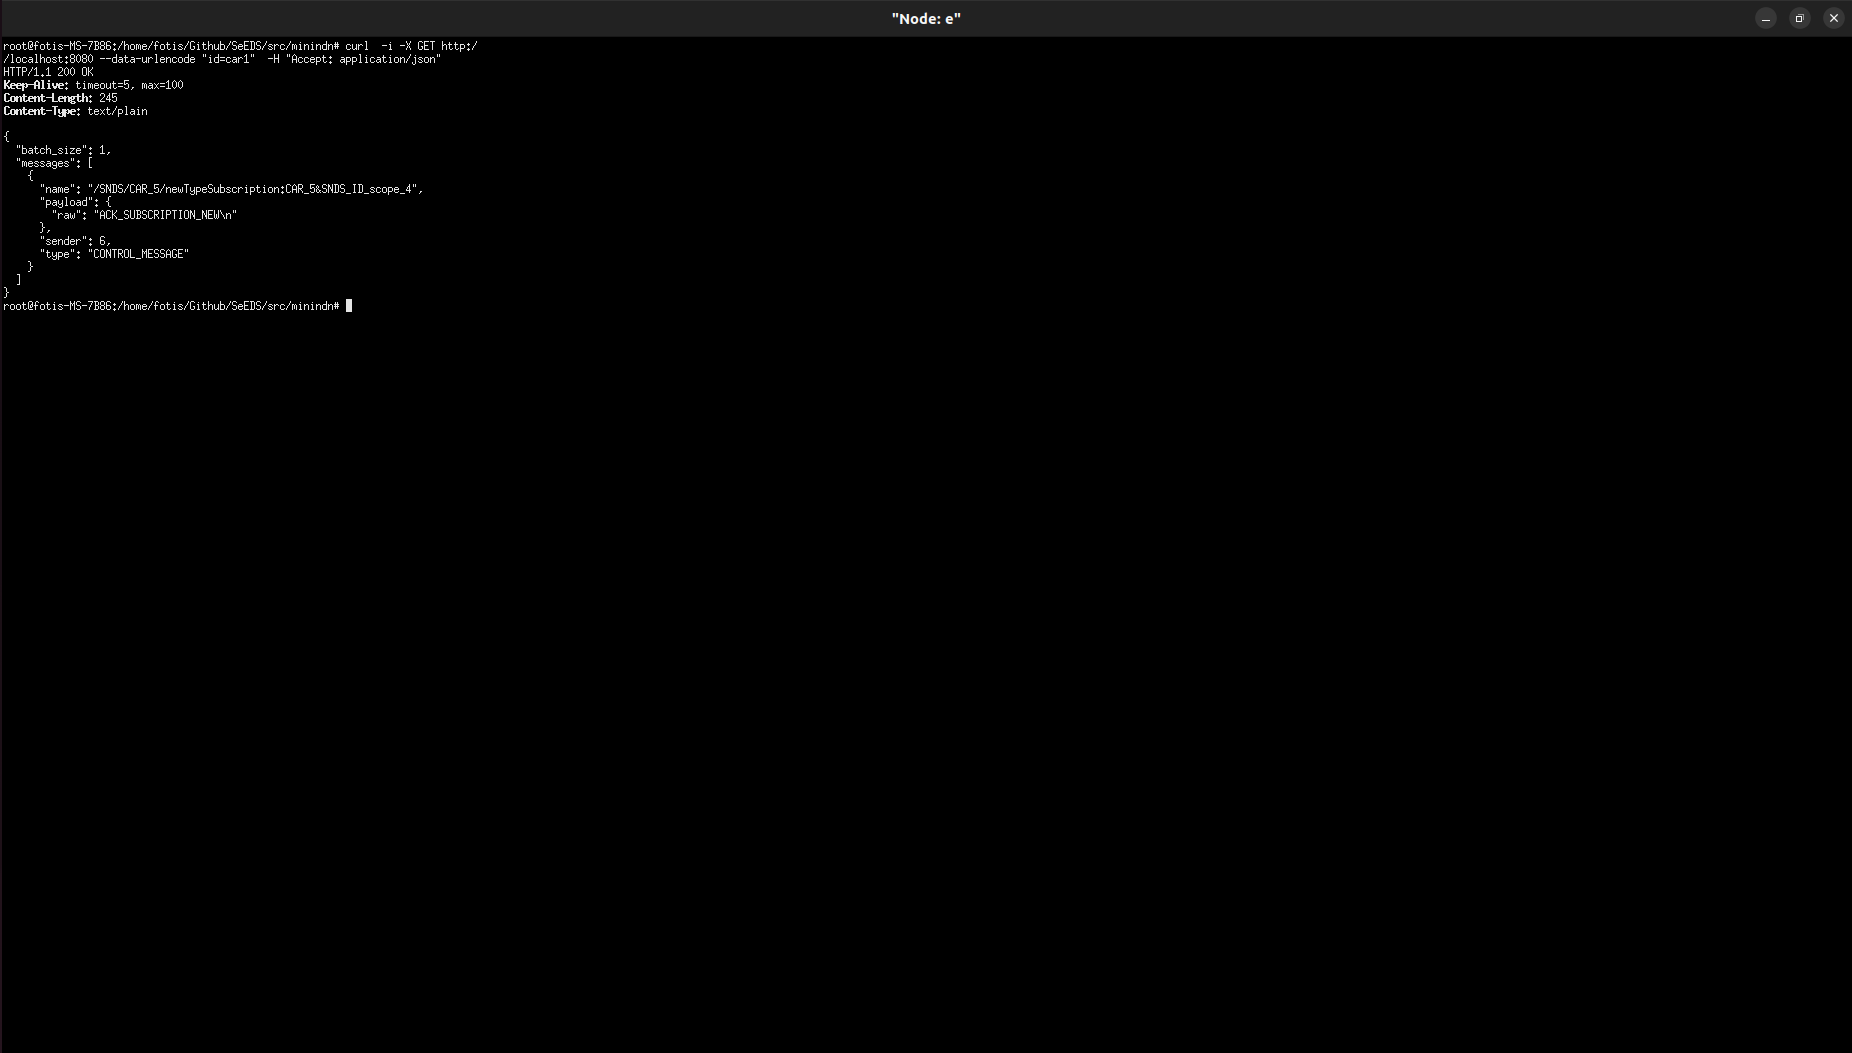
\includegraphics[width=1\linewidth]{images/after_failure_through_e.png}
    \caption{Get the data of B, which are now F's, through E}
    \label{fig:after-failure-through-e}
\end{figure}

Let's check F's logs, to see whether it actually provides the data: 

\begin{lstlisting}[language=log, caption={F logs should now provide the data originally provided through B}, label={lst:f-after-failure-provides}]
[2025-09-26 10:22:24.170] [info] [Producer] Received interest in function: onInterest, name: /SNDS/car1/temporalQuery%3Aid%3Dcar1%26type%3D%26date%3D%26count%3D%26timeframe%3D%26filters%3D
[2025-09-26 10:22:24.170] [info] [Producer] Parsed interest: Prefix: SNDS, Name: car1, Command: temporalQuery, Params: [id=car1, type=, date=, count=, timeframe=, filters=]
[2025-09-26 10:22:24.170] [debug] [Producer] Created interest response: /SNDS/car1/temporalQuery%3Aid%3Dcar1%26type%3D%26date%3D%26count%3D%26timeframe%3D%26filters%3D in: process_temporal_query_interest
[2025-09-26 10:22:24.170] [debug] [Producer] TemporalQuery → id: car1, date: , type: , timeframe: , count: , filters: 
[2025-09-26 10:22:24.170] [debug] [Producer] Requesting to endpoint: /temporal-query?id=car1&type=&count=&date=&timeframe=&filters=
[2025-09-26 10:22:24.171] [info] [Producer] Successfully queried /temporal-query
[2025-09-26 10:22:24.171] [debug] [Producer] Sending data to the NDN…
\end{lstlisting}

Let's check E's logs, to see whether it actually retrieved the data: 

\begin{lstlisting}[language=log, caption={}, label={}]
[2025-09-26 10:26:55.977] [info] [HTTPServer] Received GET request for / with body id=car1
[2025-09-26 10:26:55.977] [info] [HTTPServer] Received GET request for / with target /
[2025-09-26 10:26:55.977] [info] [HTTPServer] Received GET request from 127.0.0.1
Message: {id=car1}
Type: GET_BY_ID_REQUEST
Sender: HTTP_SRV
Payload: 
HTTP Type: HTTP_GET
Params:
id = car1
[2025-09-26 10:26:55.977] [debug] [HTTPServer] Writing message from GET request to service queue...
Message: {id=car1}
Type: GET_BY_ID_REQUEST
Sender: HTTP_SRV
Payload: 
HTTP Type: HTTP_GET
Params:
id = car1

Message: BATCH
Type: GENERIC
Sender: WORKER
Payload: {
  "batch_size": 1,
  "messages": [
    {
      "name": "/SNDS/CAR_5/newTypeSubscription:CAR_5&SNDS_ID_scope_4",
      "payload": {
        "raw": "ACK_SUBSCRIPTION_NEW\n"
      },
      "sender": 6,
      "type": "CONTROL_MESSAGE"
    }
  ]
}

HTTP Type: HTTP_EMPTY
Params:
[2025-09-26 10:26:55.977] [info] [HTTPServer] Read Message from queue:
Message: BATCH
Type: GENERIC
Sender: WORKER
Payload: {
  "batch_size": 1,
  "messages": [
    {
      "name": "/SNDS/CAR_5/newTypeSubscription:CAR_5&SNDS_ID_scope_4",
      "payload": {
        "raw": "ACK_SUBSCRIPTION_NEW\n"
      },
      "sender": 6,
      "type": "CONTROL_MESSAGE"
    }
  ]
}

HTTP Type: HTTP_EMPTY
Params:

[2025-09-26 10:26:55.977] [info] [Worker] Received content: {id=car1}
[2025-09-26 10:26:55.977] [info] [Worker] Received payload: 
[2025-09-26 10:26:55.977] [info] [Worker] Received type: GET_BY_ID_REQUEST
[2025-09-26 10:26:55.977] [debug] [Worker] Server intra message...
[2025-09-26 10:26:55.977] [info] [Worker] Inserted ID: car1 into set. Pushing regular getByID request for ID: car1
[2025-09-26 10:26:55.977] [info] [Worker] Reading packet...
[2025-09-26 10:26:55.977] [debug] [Consumer] Extracted content from message: /SNDS/car1/getByID:car1
[2025-09-26 10:26:55.977] [debug] [Consumer] Extracted content length from message: 23
[2025-09-26 10:26:55.977] [debug] [Consumer] Extracted message type from message: GET_BY_ID_REQUEST
[2025-09-26 10:26:55.977] [debug] [Consumer] Query.type: 
[2025-09-26 10:26:55.977] [debug] [Consumer] Query.id: car1
[2025-09-26 10:26:55.977] [info] [Consumer] Created name /SNDS/car1/temporalQuery:id%3Dcar1&type%3D&date%3D&count%3D&timeframe%3D&filters%3D
[2025-09-26 10:26:55.977] [info] [Consumer] Sending actual Interest /SNDS/car1/temporalQuery%3Aid%3Dcar1%26type%3D%26date%3D%26count%3D%26timeframe%3D%26filters%3D?CanBePrefix&Lifetime=6000
[2025-09-26 10:26:55.977] [info] [Consumer] Received Data with name: /SNDS/car1/temporalQuery%3Aid%3Dcar1%26type%3D%26date%3D%26count%3D%26timeframe%3D%26filters%3D in function onData
[2025-09-26 10:26:55.977] [info] [Consumer] Data packet payload: [
  {
    "": {
      "_id": "car1",
      "id": "car1",
      "timestamp": {
        "$date": 1758870079983
      },
      "type": "GENERIC"
    }
  }
] in function onData
[2025-09-26 10:26:55.977] [info] [Consumer] Parsed interest: Prefix: SNDS, Name: car1, Command: temporalQuery, Params: [id=car1, type=, date=, count=, timeframe=, filters=] in onData
[2025-09-26 10:26:55.977] [info] [Consumer] Temporal Query Reponse...
[2025-09-26 10:26:55.977] [debug] [Consumer] Removed extra characters from payload (first 32 bytes hex): 5b 0a 20 20 7b 0a 20 20 20 20 22 22 3a 20 7b 0a 20 20 20 20 20 20 22 5f 69 64 22 3a 20 22 63 61 
[2025-09-26 10:26:55.977] [debug] [Consumer] Candidate JSON slice:
[
  {
    "": {
      "_id": "car1",
      "id": "car1",
      "timestamp": {
        "$date": 1758870079983
      },
      "type": "GENERIC"
    }
  }
]
[2025-09-26 10:26:55.977] [debug] [Consumer] Sanitized payload to:
[
  {
    "": {
      "_id": "car1",
      "id": "car1",
      "timestamp": {
        "$date": 1758870079983
      },
      "type": "GENERIC"
    }
  }
]
\end{lstlisting}

Nice E got the data back!

Finally let's also check the time of failure of \emph{Primary Node} C and the recovery of \emph{Secondary Node} G:

\begin{lstlisting}[language=log, caption={Timeout of Node C}, label={lst:timeout-node-c}]
[TIMEOUT] 2025-09-26 10:03:14.265 c: daemon exceeded timeout 
\end{lstlisting}

\begin{lstlisting}[language=log, caption={Recovery of Node C through Node G}, label={lst:recovery-of-node-c-g}]
[2025-09-26 10:03:14.281] [warning] [Producer] [resilience-ipc] promotion to PRIMARY (reason=alive-missed, misses=1)
[2025-09-26 10:03:14.281] [info] [Producer] [resilience] mutate → ver=6 hash=be7008804c441ae38b5c667e74638083
[2025-09-26 10:03:14.281] [debug] [Producer] [resilience] history versions: 0(37a6259c) 1(e9af7cdf) 2(721c5a31) 3(1743154a) 4(8a357a28) 5(a3baea0e) 6(be700880) 
[2025-09-26 10:03:14.281] [debug] [Producer] [resilience] ops from v5 → v6:
[
  {
    "op": "replace",
    "path": "/resilience/reason",
    "value": "alive-missed"
  },
  {
    "op": "replace",
    "path": "/resilience/role",
    "value": "primary"
  },
  {
    "op": "replace",
    "path": "/resilience/since",
    "value": "2025-09-26T07:03:14Z"
  },
  {
    "op": "add",
    "path": "/resilience/misses",
    "value": 1
  }
]
[2025-09-26 10:03:14.281] [warning] [Producer] [resilience-ipc] stop requested; will be joined from main loop
[2025-09-26 10:03:14.320] [warning] [Producer] [resilience] applying promotion side-effects on main loop
[2025-09-26 10:03:14.320] [debug] [Producer] [overlay] merge: applying json_patch_against_base (ops=7)
[2025-09-26 10:03:14.320] [debug] [Producer] [resilience] assign → ver=7 hash=75a517298fe7436e7751682d14c27144
[2025-09-26 10:03:14.320] [debug] [Producer] [overlay] SQUASH → base version 6→7  hash be7008804c441ae38b5c667e74638083→75a517298fe7436e7751682d14c27144  overlay ver=16 hash=6f373a7c7c0c7f801932225586b6fa4f
[2025-09-26 10:03:14.320] [debug] [Producer] [overlay] CLEARED
[2025-09-26 10:03:14.320] [debug] [Producer] [promotion] rebuilt containers from store:
[2025-09-26 10:03:14.320] [debug] [Producer]   type_registry[CAR_2] = [car12 ]
[2025-09-26 10:03:14.320] [debug] [Producer]   type_registry[CAR_6] = [car16 ]
[2025-09-26 10:03:14.320] [debug] [Producer]   subscribed_nodes_for_type[CAR_2] = [SNDS_ID_scope_1 ]
[2025-09-26 10:03:14.320] [debug] [Producer]   subscribed_nodes_for_type[CAR_6] = [SNDS_ID_scope_5 ]
[2025-09-26 10:03:14.320] [debug] [Producer]   announcements = [/SNDS_2 /SNDS/CAR_6 /SNDS_6 /SNDS/car6 /SNDS/car2 /SNDS/SNDS_ID_scope_6 /SNDS/is_alive_6 /SNDS/CAR_6_registry /SNDS/state_6 /SNDS/CAR_2 /SNDS/state_2 /SNDS/CAR_2_registry /SNDS/SNDS_ID_scope_2 /SNDS/is_alive_2 ]
[2025-09-26 10:03:14.320] [info] [Producer] [promotion] summary: types=2 ids=2 subs(byId)=0 subs(byType)=2 announced=14
[2025-09-26 10:03:14.320] [info] [Producer] [promotion] (re)announcing /SNDS_2
[2025-09-26 10:03:14.320] [info] [Producer] [promotion] (re)announcing /SNDS/CAR_6
[2025-09-26 10:03:14.320] [info] [Producer] [promotion] (re)announcing /SNDS_6
[2025-09-26 10:03:14.320] [info] [Producer] [promotion] (re)announcing /SNDS/car6
[2025-09-26 10:03:14.321] [info] [Producer] [promotion] (re)announcing /SNDS/car2
[2025-09-26 10:03:14.321] [info] [Producer] [promotion] (re)announcing /SNDS/SNDS_ID_scope_6
[2025-09-26 10:03:14.321] [info] [Producer] [promotion] (re)announcing /SNDS/is_alive_6
[2025-09-26 10:03:14.321] [info] [Producer] [promotion] (re)announcing /SNDS/CAR_6_registry
[2025-09-26 10:03:14.321] [info] [Producer] [promotion] (re)announcing /SNDS/state_6
[2025-09-26 10:03:14.321] [info] [Producer] [promotion] (re)announcing /SNDS/CAR_2
[2025-09-26 10:03:14.321] [info] [Producer] [promotion] (re)announcing /SNDS/state_2
[2025-09-26 10:03:14.321] [info] [Producer] [promotion] (re)announcing /SNDS/CAR_2_registry
[2025-09-26 10:03:14.321] [info] [Producer] [promotion] (re)announcing /SNDS/SNDS_ID_scope_2
[2025-09-26 10:03:14.322] [info] [Producer] [promotion] (re)announcing /SNDS/is_alive_2
[2025-09-26 10:03:14.322] [info] [Producer] Getting from IP: 10.0.0.42 and port: 10000
[2025-09-26 10:03:14.322] [debug] [Producer] HTTP GET /state?type=CAR_2
[2025-09-26 10:03:14.324] [info] [Producer] [resilience] mutate → ver=8 hash=8e464c8782cf6591d70ef4f5885d1acb
[2025-09-26 10:03:14.324] [debug] [Producer] [resilience] history versions: 0(37a6259c) 1(e9af7cdf) 2(721c5a31) 3(1743154a) 4(8a357a28) 5(a3baea0e) 6(be700880) 7(75a51729) 8(8e464c87) 
[2025-09-26 10:03:14.324] [debug] [Producer] [resilience] ops from v7 → v8:
[
  {
    "op": "replace",
    "path": "/broker/collections/CAR_2/lastSeen",
    "value": "2025-09-26T07:03:14Z"
  }
]
[2025-09-26 10:03:14.324] [info] [Producer] Getting from IP: 10.0.0.42 and port: 10000
[2025-09-26 10:03:14.324] [debug] [Producer] HTTP GET /state?type=CAR_6
[2025-09-26 10:03:14.325] [info] [Producer] [resilience] mutate → ver=9 hash=8d00fd7121cc9637c59c2b2698b4f4fb
[2025-09-26 10:03:14.325] [debug] [Producer] [resilience] history versions: 0(37a6259c) 1(e9af7cdf) 2(721c5a31) 3(1743154a) 4(8a357a28) 5(a3baea0e) 6(be700880) 7(75a51729) 8(8e464c87) 9(8d00fd71) 
[2025-09-26 10:03:14.325] [debug] [Producer] [resilience] ops from v8 → v9:
[
  {
    "op": "add",
    "path": "/broker/collections/CAR_6",
    "value": {
      "algo": "SHA-256",
      "count": 0,
      "hash": "e3b0c44298fc1c149afbf4c8996fb92427ae41e4649b934ca495991b7852b855",
      "lastSeen": "2025-09-26T07:03:14Z"
    }
  }
]
[2025-09-26 10:03:14.327] [info] [Producer] Successfully registered prefix: /SNDS_2
[2025-09-26 10:03:14.327] [info] [Producer] Successfully registered prefix: /SNDS/CAR_6
[2025-09-26 10:03:14.327] [info] [Producer] Successfully registered prefix: /SNDS_6
[2025-09-26 10:03:14.327] [info] [Producer] Successfully registered prefix: /SNDS/car6
[2025-09-26 10:03:14.327] [info] [Producer] Successfully registered prefix: /SNDS/car2
[2025-09-26 10:03:14.328] [info] [Producer] Successfully registered prefix: /SNDS/SNDS_ID_scope_6
[2025-09-26 10:03:14.329] [info] [Producer] Successfully registered prefix: /SNDS/is_alive_6
[2025-09-26 10:03:14.329] [info] [Producer] Successfully registered prefix: /SNDS/CAR_6_registry
[2025-09-26 10:03:14.329] [info] [Producer] Successfully registered prefix: /SNDS/state_6
[2025-09-26 10:03:14.329] [info] [Producer] Successfully registered prefix: /SNDS/CAR_2
[2025-09-26 10:03:14.330] [info] [Producer] Successfully registered prefix: /SNDS/state_2
[2025-09-26 10:03:14.330] [info] [Producer] Successfully registered prefix: /SNDS/CAR_2_registry
[2025-09-26 10:03:14.330] [info] [Producer] Successfully registered prefix: /SNDS/SNDS_ID_scope_2
[2025-09-26 10:03:14.330] [info] [Producer] Successfully registered prefix: /SNDS/is_alive_2 
\end{lstlisting}

C's failure log is at: \textbf{2025-09-26 10:03:14.265} and G's last data recovered is at: \textbf{2025-09-26 10:03:14.330}. This gives us a difference of \textit{65ms}.

The resilience evaluation demonstrated that the SeEDS system effectively recovers from transient disruptions under \emph{200\,ms}. Following recovery, the synchronization mechanism between the \emph{Primary} and \emph{Secondary} nodes is restored, ensuring that the latest state of the data maintained by the Primary nodes becomes accessible through their corresponding Secondary replicas. This confirms that SeEDS maintains data availability and consistency even in the presence of short-lived network or service interruptions, thereby validating its robustness and reliability in distributed environments.

\subsection{NDN-testbed (KPI 6)}
To satisfy KPI 6, we deployed and tested the SeEDS prototype in the official NDN testbed. The experiment involved a distributed setup with three participating nodes that interconnect through the NDN across three different continents, including the University of Memphis (UMemphis) testbed node.

The prototype we tested included the \emph{GET by TYPE} and \emph{GET by ID} requests. The other requests have also been tested locally in MiniNDN and work as expected. Future work will include testing the other request types in the testbed network.

The experiment demonstrated end-to-end communication between the nodes, ensuring that Interests and Data packets could be exchanged reliably across wide-area NDN infrastructure.This deployment validated:

\begin{itemize}
    \item The ability of SeEDS to operate in a multi-continental environment.
    \item Correct operation of the system in the global NDN testbed, beyond controlled lab conditions.
    \item Successful integration of the UMemphis node as a critical participant in the experiment.
\end{itemize}

\subsubsection{Topology}

The experiment was deployed on the NDN testbed using a three-node topology spanning different continents in NDN hops. The participating nodes were:

\begin{itemize}
    \item \emph{MMLab1} – NDN testbed node located in Athens University of Economics and , was configured as the Producer node, responsible for publishing and advertising data into the NDN network.
    \item \emph{MMLab2} – NDN testbed node located again in Athens University of Economics and Business, issuing Interests to retrieve data from the producer.
    \item \emph{UMemphis} – NDN testbed node located in North America (University of Memphis), was configured as a Consumer node, retrieving the same data across transcontinental paths.
\end{itemize}

The full topology can be found in: https://play.ndn.today/?testbed=1. The below topology has been simplified to contain a max of 3 hops distance from the \emph{MMLab} NDN nodes to the \emph{Memphis} NDN node. We can also include all distances, but these are the most likely paths a NDN packet is going to take. Note we also keep the consumer node \emph{MMLab2} connections with consumer \emph{Memphis}, because the \emph{Memphis} node might be able to retrieve data from the cache of \emph{MMLab2}.

\begin{figure}[H]
    \centering
    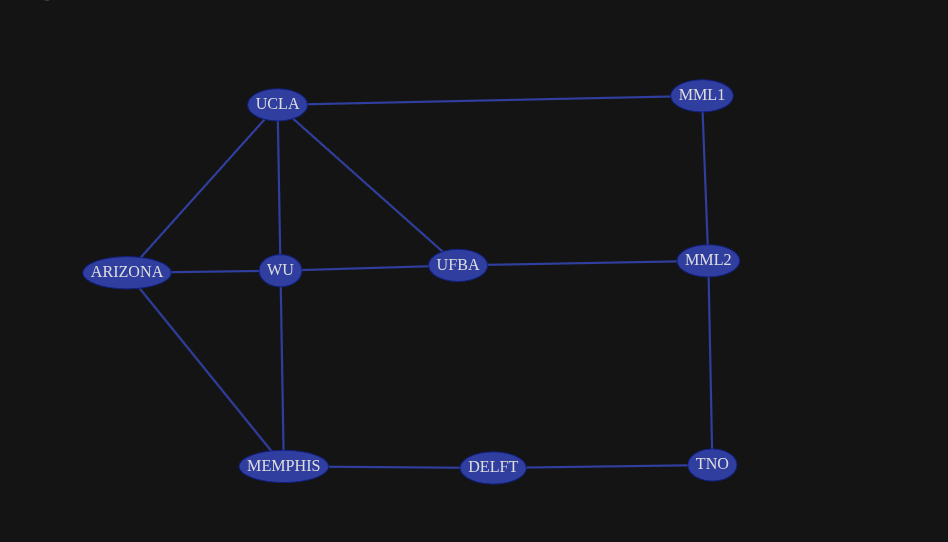
\includegraphics[width=1\linewidth]{images/ndntestbed_topology.png}
    \caption{Simplified 3-hop NDN testbed topology showing the main paths between producer (\emph{MMLab1}) and consumers (\emph{MMLab2, UMemphis}), with potential intermediate relay/caching nodes.}
    \label{fig:ndntestbed_topology}
\end{figure}

\begin{itemize}
    \item UFBA: Federal University of Bahia in Brazil - South America.
    \item UCLA: University of California in Los Angeles - United States - North America.
    \item WU: Washington University in St.Louis - United States - North America.
    \item TNO: Netherlands Organisation for Applied Scientific Research - Europe
    \item DELFT: Delft University of Technology in Netherlands - Europe.
    \item ARIZONA: University of Arizona - North America.
\end{itemize}


Based on the graph and the routing tables at least two continents are involved in the communication between Memphis and the MMLab nodes, with the possibility that a third continent South America is going to be involved in the communication. This topology ensured intercontinental communication paths, with each node positioned in a different geographic region. If the data between the nodes can be retrieved, the intercontinental communication is possible. Note that the MiniNDN links are set up like this:
\pagebreak
\begin{lstlisting}[language=minindnconf, caption={MiniNDN config file for the testbed nodes}, label={lst:minindn-conf-testbed}]
[nodes]
UCLA: _ network=/world router=/UCLA.Router/ position=-40.5,-28.7,0
TNO: _ network=/world router=/TNO.Router/ position=-0.1,4.8,0
MEMPHIS: _ network=/world router=/MEMPHIS.Router/ position=-39.9,5,0
UFBA: _ network=/world router=/UFBA.Router/ position=-23.7,-13.7,0
MML2: _ network=/world router=/MML2.Router/ position=-0.5,-14.2,0
MML1: _ network=/world router=/MML1.Router/ position=-1,-29.5,0
ARIZONA: _ network=/world router=/ARIZONA.Router/ position=-54.5,-13,0
DELFT: _ network=/world router=/DELFT.Router/ position=-20.5,5.1,0
WU: _ network=/world router=/WU.Router/ position=-40.2,-13.2,0
[switches]
[links]
UCLA:MML1 delay=10ms
UCLA:ARIZONA delay=10ms
UCLA:WU delay=10ms
UCLA:UFBA delay=10ms
TNO:DELFT delay=10ms
TNO:MML2 delay=10ms
MEMPHIS:ARIZONA delay=10ms
MEMPHIS:WU delay=10ms
MEMPHIS:DELFT delay=10ms
UFBA:WU delay=10ms
UFBA:MML2 delay=10ms
MML2:MML1 delay=10ms
ARIZONA:WU delay=10ms 
\end{lstlisting}

\subsubsection{GET by ID}

In this experiment, the entity \textit{@id=car001} is published directly by the Producer node (\textit{MMLab1}), thereby registering it within the Producer’s local namespace and enabling retrieval by other nodes across the network.

Let's publish \textit{@id=car001} to the network: 

\begin{lstlisting}[language=curl, caption={Publish \textit{@id=car001} to the NDN network through the Producer Node}, label={lst:publish-id-testbed}]
scn4ndn@seeds8:~$ curl -v -i -X POST http://127.0.0.1:8080 -d "id=car001"
Note: Unnecessary use of -X or --request, POST is already inferred.
*   Trying 127.0.0.1:8080...
* Connected to 127.0.0.1 (127.0.0.1) port 8080
> POST / HTTP/1.1
> Host: 127.0.0.1:8080
> User-Agent: curl/8.5.0
> Accept: */*
> Content-Length: 9
> Content-Type: application/x-www-form-urlencoded
> 
< HTTP/1.1 200 OK
HTTP/1.1 200 OK
< Keep-Alive: timeout=5, max=100
Keep-Alive: timeout=5, max=100
< Content-Length: 189
Content-Length: 189
< Content-Type: text/plain
Content-Type: text/plain

< 
{
  "batch_size": 1,
  "messages": [
    {
      "name": "",
      "payload": {
        "raw": "ACK_ID_ADVERTISED\n"
      },
      "sender": 6,
      "type": "CONTROL_MESSAGE"
    }
  ]
}
* Connection #0 to host 127.0.0.1 left intact 
\end{lstlisting}

Let's check the logs from within the SeEDS Service of the Producer: 

\begin{lstlisting}[language=log, caption={SeEDS Service logs of the Producer after publishing \textit{@id=car001} }, label={lst:service-logs-after-car001}]
[2025-10-01 13:49:06.864] [info] [HTTPServer] Received POST request for / with body id=car001
[2025-10-01 13:49:06.864] [info] [HTTPServer] Received POST request from 127.0.0.1
Message: {id=car001}
Type: BY_ID_ADVERTISEMENT
Sender: HTTP_SRV
Payload: 
HTTP Type: HTTP_POST
Params:
id = car001
[2025-10-01 13:49:06.864] [debug] [HTTPServer] Writing message from POST request to service queue...
Message: {id=car001}
Type: BY_ID_ADVERTISEMENT
Sender: HTTP_SRV
Payload: 
HTTP Type: HTTP_POST
Params:
id = car001

[2025-10-01 13:49:06.864] [debug] [DigitalTwin] Extracted content from message {id=car001}
[2025-10-01 13:49:06.864] [debug] [DigitalTwin] Extracted content length from message 11
[2025-10-01 13:49:06.864] [debug] [DigitalTwin] Extracted type from message: BY_ID_ADVERTISEMENT
[2025-10-01 13:49:06.864] [info] [DigitalTwin] Received by ID get request...
[2025-10-01 13:49:06.864] [debug] [DigitalTwin] Pushed ID car001 to the announced IDs vector...
[2025-10-01 13:49:06.864] [debug] [DigitalTwin] Extracted id Scope from message SNDS_ID_scope_2
Message: /ndn/gr/edu/mmlab1/aueb/thomasi/car001/postID:car001
Type: BY_ID_ADVERTISEMENT
Sender: DIGITAL_TWIN
Payload: 
HTTP Type: HTTP_EMPTY
Params:
[2025-10-01 13:49:06.864] [info] [DigitalTwin] Pushing byID advertisement to the Producer...
Message: /ndn/gr/edu/mmlab1/aueb/thomasi/car001/postID:car001
Type: BY_ID_ADVERTISEMENT
Sender: DIGITAL_TWIN
Payload: 
HTTP Type: HTTP_EMPTY
Params:

[2025-10-01 13:49:06.864] [debug] [DigitalTwin] Sleeping 2000 ms before sending scope advertisement...
Message: /ndn/gr/edu/mmlab1/aueb/thomasi/car001/postID:car001
Type: BY_ID_ADVERTISEMENT
Sender: DIGITAL_TWIN
Payload: 
HTTP Type: HTTP_EMPTY
Params:
[2025-10-01 13:49:06.893] [info] [Producer] Got new ID advertisement request...
Message: /ndn/gr/edu/mmlab1/aueb/thomasi/car001/postID:car001
Type: BY_ID_ADVERTISEMENT
Sender: DIGITAL_TWIN
Payload: 
HTTP Type: HTTP_EMPTY
Params:

[2025-10-01 13:49:06.893] [debug] [Producer] Parsed interest Prefix: ndn/gr/edu/mmlab1/aueb/thomasi, Name: car001, Command: postID, Params: [car001] from string
[2025-10-01 13:49:06.893] [info] [Producer] Announcing name: /ndn/gr/edu/mmlab1/aueb/thomasi/car001
[2025-10-01 13:49:06.894] [info] [Producer] Publishing to broker...
[2025-10-01 13:49:06.894] [warning] [Producer] _publish_to_broker: 'type' (string) not provided...
[2025-10-01 13:49:06.894] [info] [Producer] POST /add -> {"id":"car001"}
[2025-10-01 13:49:07.082] [info] [Producer] Published to broker OK: {"status": "success", "inserted_count_versioned": 1, "upserted_or_modified_count": 1}

[2025-10-01 13:49:07.082] [debug] [Producer] Appending body to broker journal: {"id":"car001"}
[2025-10-01 13:49:07.082] [info] [Producer] [resilience] mutate → ver=8 hash=a96596e77b8ca3a9df6378a6ef9a4362
[2025-10-01 13:49:07.082] [debug] [Producer] [resilience] history versions: 0(37a6259c) 1(5b784e73) 2(851bb2ce) 3(f2dc8068) 4(1dbec4b9) 5(92323da8) 6(a8c74cc9) 7(11cc7dd5) 8(a96596e7) 
[2025-10-01 13:49:07.082] [debug] [Producer] [resilience] ops from v7 → v8:
[
  {
    "op": "add",
    "path": "/broker/journal",
    "value": [
      {
        "id": "car001",
        "payload": {
          "id": "car001"
        },
        "ts": "2025-10-01T13:49:07Z",
        "type": "GENERIC"
      }
    ]
  }
]
[2025-10-01 13:49:07.083] [info] [Worker] Received content: 
[2025-10-01 13:49:07.083] [info] [Worker] Received payload: ACK_ID_ADVERTISED
[2025-10-01 13:49:07.083] [info] [Worker] Received type: BY_ID_ADVERTISEMENT
[2025-10-01 13:49:07.083] [info] [Worker] Received ACK Message with name:  payload: ACK_ID_ADVERTISED...
Message: 
Type: CONTROL_MESSAGE
Sender: WORKER
Payload: ACK_ID_ADVERTISED

HTTP Type: HTTP_EMPTY
Params:
[2025-10-01 13:49:07.083] [debug] [Worker] Writing message to service queue:
Message: 
Type: CONTROL_MESSAGE
Sender: WORKER
Payload: ACK_ID_ADVERTISED

HTTP Type: HTTP_EMPTY
Params:

[2025-10-01 13:49:07.083] [info] [Worker] Reading packet...
Message: BATCH
Type: GENERIC
Sender: WORKER
Payload: {
  "batch_size": 1,
  "messages": [
    {
      "name": "",
      "payload": {
        "raw": "ACK_ID_ADVERTISED\n"
      },
      "sender": 6,
      "type": "CONTROL_MESSAGE"
    }
  ]
}

HTTP Type: HTTP_EMPTY
Params:
[2025-10-01 13:49:07.083] [info] [HTTPServer] Read Message from queue:
Message: BATCH
Type: GENERIC
Sender: WORKER
Payload: {
  "batch_size": 1,
  "messages": [
    {
      "name": "",
      "payload": {
        "raw": "ACK_ID_ADVERTISED\n"
      },
      "sender": 6,
      "type": "CONTROL_MESSAGE"
    }
  ]
}

HTTP Type: HTTP_EMPTY
Params:

[2025-10-01 13:49:07.087] [info] [Producer] Successfully registered prefix: /ndn/gr/edu/mmlab1/aueb/thomasi/car001 
\end{lstlisting}

Let's try to GET the \textit{@id=car001} from the SeEDS Service of Consumer \emph{MMLab2}:
\begin{lstlisting}[language=curl, caption={GET by ID for \textit{@id=car001} through Node \emph{MMlab2}}, label={lst:http-request-mmlab2-car001}]
scn4ndn@seeds7:~$ curl -i -X GET http://localhost:8080/?"id=car001"
HTTP/1.1 200 OK
Keep-Alive: timeout=5, max=100
Content-Length: 332
Content-Type: text/plain

{
  "batch_size": 1,
  "messages": [
    {
      "name": "",
      "payload": {
        "items": [
          {
            "date": 1759326546992,
            "id": "car001",
            "type": "GENERIC"
          }
        ],
        "mode": "direct"
      },
      "sender": 6,
      "type": "TEMPORAL_QUERY_RESPONSE"
    }
  ]
} 
\end{lstlisting}

Nice we got the ID. Let's make sure we actually got it from the \emph{Producer Node}. Let's check the logs of the \emph{Producer}:

\begin{lstlisting}[language=log, caption={Producer logs after receiving GET by ID from \emph{MMLab2}}, label={lst:producer-logs-get-by-id-car001}]
[2025-10-01 13:50:41.971] [info] [Producer] Received interest in function: onInterest, name: /ndn/gr/edu/mmlab1/aueb/thomasi/car001/temporalQuery%3Aid%3Dcar001%26type%3D%26date%3D%26count%3D%26timeframe%3D%26filters%3D
[2025-10-01 13:50:41.971] [info] [Producer] Parsed interest: Prefix: ndn/gr/edu/mmlab1/aueb/thomasi, Name: car001, Command: temporalQuery, Params: [id=car001, type=, date=, count=, timeframe=, filters=]
[2025-10-01 13:50:41.971] [debug] [Producer] Created interest response: /ndn/gr/edu/mmlab1/aueb/thomasi/car001/temporalQuery%3Aid%3Dcar001%26type%3D%26date%3D%26count%3D%26timeframe%3D%26filters%3D in: process_temporal_query_interest
[2025-10-01 13:50:41.971] [debug] [Producer] TemporalQuery → id: car001, date: , type: , timeframe: , count: , filters: 
[2025-10-01 13:50:41.971] [debug] [Producer] Requesting to endpoint: /temporal-query?id=car001&type=&count=&date=&timeframe=&filters=
[2025-10-01 13:50:41.972] [info] [Producer] Successfully queried /temporal-query
[2025-10-01 13:50:41.972] [debug] [Producer] Sending data to the NDN… 
\end{lstlisting}

Let's also check the logs of \emph{MMLab2} SeEDS Service:

\begin{lstlisting}[language=log, caption={After GET by ID of \textit{@id=car001} and response from \emph{MMLab1}-Producer}, label={lst:consumer-logs-get-by-id-car001}]
[2025-10-01 13:50:41.969] [info] [HTTPServer] Received GET request for / with body 
[2025-10-01 13:50:41.969] [info] [HTTPServer] Received GET request for / with target /?id=car001
[2025-10-01 13:50:41.969] [info] [HTTPServer] Received GET request from 127.0.0.1
Message: {id=car001}
Type: GET_BY_ID_REQUEST
Sender: HTTP_SRV
Payload: 
HTTP Type: HTTP_GET
Params:
id = car001
[2025-10-01 13:50:41.969] [debug] [HTTPServer] Writing message from GET request to service queue...
Message: {id=car001}
Type: GET_BY_ID_REQUEST
Sender: HTTP_SRV
Payload: 
HTTP Type: HTTP_GET
Params:
id = car001

[2025-10-01 13:50:41.969] [info] [Worker] Received content: {id=car001}
[2025-10-01 13:50:41.969] [info] [Worker] Received payload: 
[2025-10-01 13:50:41.969] [info] [Worker] Received type: GET_BY_ID_REQUEST
[2025-10-01 13:50:41.969] [debug] [Worker] Server intra message...
[2025-10-01 13:50:41.969] [info] [Worker] Inserted ID: car001 into set. Pushing regular getByID request for ID: car001
[2025-10-01 13:50:41.969] [info] [Worker] Reading packet...
[2025-10-01 13:50:41.969] [debug] [Consumer] Extracted content from message: /ndn/gr/edu/mmlab1/aueb/thomasi/car001/getByID:car001
[2025-10-01 13:50:41.969] [debug] [Consumer] Extracted content length from message: 53
[2025-10-01 13:50:41.969] [debug] [Consumer] Extracted message type from message: GET_BY_ID_REQUEST
[2025-10-01 13:50:41.969] [debug] [Consumer] Query.type: 
[2025-10-01 13:50:41.969] [debug] [Consumer] Query.id: car001
[2025-10-01 13:50:41.969] [info] [Consumer] Created name /ndn/gr/edu/mmlab1/aueb/thomasi/car001/temporalQuery:id%3Dcar001&type%3D&date%3D&count%3D&timeframe%3D&filters%3D
[2025-10-01 13:50:41.969] [info] [Consumer] Sending actual Interest /ndn/gr/edu/mmlab1/aueb/thomasi/car001/temporalQuery%3Aid%3Dcar001%26type%3D%26date%3D%26count%3D%26timeframe%3D%26filters%3D?CanBePrefix&MustBeFresh&Lifetime=200
[2025-10-01 13:50:41.977] [info] [Consumer] Received Data with name: /ndn/gr/edu/mmlab1/aueb/thomasi/car001/temporalQuery%3Aid%3Dcar001%26type%3D%26date%3D%26count%3D%26timeframe%3D%26filters%3D in function onData
[2025-10-01 13:50:41.977] [info] [Consumer] Data packet payload: [
  {
    "": {
      "_id": "car001",
      "id": "car001",
      "timestamp": {
        "$date": 1759326546992
      },
      "type": "GENERIC"
    }
  }
] in function onData
[2025-10-01 13:50:41.977] [info] [Consumer] Parsed interest: Prefix: ndn/gr/edu/mmlab1/aueb/thomasi, Name: car001, Command: temporalQuery, Params: [id=car001, type=, date=, count=, timeframe=, filters=] in onData
[2025-10-01 13:50:41.977] [info] [Consumer] Temporal Query Reponse...
[2025-10-01 13:50:41.977] [debug] [Consumer] Removed extra characters from payload (first 32 bytes hex): 5b 0a 20 20 7b 0a 20 20 20 20 22 22 3a 20 7b 0a 20 20 20 20 20 20 22 5f 69 64 22 3a 20 22 63 61 
[2025-10-01 13:50:41.977] [debug] [Consumer] Candidate JSON slice:
[
  {
    "": {
      "_id": "car001",
      "id": "car001",
      "timestamp": {
        "$date": 1759326546992
      },
      "type": "GENERIC"
    }
  }
]
[2025-10-01 13:50:41.977] [debug] [Consumer] Sanitized payload to:
[
  {
    "": {
      "_id": "car001",
      "id": "car001",
      "timestamp": {
        "$date": 1759326546992
      },
      "type": "GENERIC"
    }
  }
]
[2025-10-01 13:50:41.977] [debug] [Consumer] Direct mode (single id in bucket).
[2025-10-01 13:50:41.977] [debug] [Consumer] Got ID and type in direct: id=car001,type=
[2025-10-01 13:50:41.978] [info] [Worker] Received content: /?id=car001&type=&date=&metafile=false&parentQueryHash=&lastInterest=true&mode=direct
[2025-10-01 13:50:41.978] [info] [Worker] Received payload: [
  {
    "": {
      "_id": "car001",
      "id": "car001",
      "timestamp": {
        "$date": 1759326546992
      },
      "type": "GENERIC"
    }
  }
]
[2025-10-01 13:50:41.978] [info] [Worker] Received type: VERSION_RESPONSE
[2025-10-01 13:50:41.978] [debug] [Worker] Consumer intra message...
[2025-10-01 13:50:41.978] [info] [Worker] Direct mode...
[2025-10-01 13:50:41.978] [info] [Consumer] Reading packet...
[2025-10-01 13:50:41.978] [debug] [Worker] Cleared pending_get_by_id_requests for 'car001': erased=1
[2025-10-01 13:50:41.978] [debug] [Worker] Cleared pending_get_by_type_requests for 'GENERIC': erased=0
[2025-10-01 13:50:41.978] [debug] [Worker] Direct mode: no filters discovered; returning full item
[2025-10-01 13:50:41.978] [info] [Worker] Reading packet...
Message: BATCH
Type: GENERIC
Sender: WORKER
Payload: {
  "batch_size": 1,
  "messages": [
    {
      "name": "",
      "payload": {
        "items": [
          {
            "date": 1759326546992,
            "id": "car001",
            "type": "GENERIC"
          }
        ],
        "mode": "direct"
      },
      "sender": 6,
      "type": "TEMPORAL_QUERY_RESPONSE"
    }
  ]
}

HTTP Type: HTTP_EMPTY
Params:
[2025-10-01 13:50:41.978] [info] [HTTPServer] Read Message from queue:
Message: BATCH
Type: GENERIC
Sender: WORKER
Payload: {
  "batch_size": 1,
  "messages": [
    {
      "name": "",
      "payload": {
        "items": [
          {
            "date": 1759326546992,
            "id": "car001",
            "type": "GENERIC"
          }
        ],
        "mode": "direct"
      },
      "sender": 6,
      "type": "TEMPORAL_QUERY_RESPONSE"
    }
  ]
}

HTTP Type: HTTP_EMPTY
Params: 
\end{lstlisting}


Let's also try to get it from the \emph{UMemphis} Node: 

\begin{lstlisting}[language=curl, caption={HTTP Request for \textit{@id=car001} }, label={lst:umemphis-http-request-car001}]
scn4ndn@seeds23:~$ curl -i -X GET http://localhost:8080/?"id=car001"
HTTP/1.1 200 OK
Keep-Alive: timeout=5, max=100
Content-Length: 332
Content-Type: text/plain

{
  "batch_size": 1,
  "messages": [
    {
      "name": "",
      "payload": {
        "items": [
          {
            "date": 1759326546992,
            "id": "car001",
            "type": "GENERIC"
          }
        ],
        "mode": "direct"
      },
      "sender": 6,
      "type": "TEMPORAL_QUERY_RESPONSE"
    }
  ]
}
scn4ndn@seeds23:~$  
\end{lstlisting}

Let's check the Producer's SeEDS Service logs: 

\begin{lstlisting}[language=log, caption={Logs after receiving GET by ID request from node \emph{UMemphis}}, label={lst:producer-get-by-id-after-umemphis}]
[2025-10-01 13:53:00.664] [info] [Producer] Received interest in function: onInterest, name: /ndn/gr/edu/mmlab1/aueb/thomasi/car001/temporalQuery%3Aid%3Dcar001%26type%3D%26date%3D%26count%3D%26timeframe%3D%26filters%3D
[2025-10-01 13:53:00.664] [info] [Producer] Parsed interest: Prefix: ndn/gr/edu/mmlab1/aueb/thomasi, Name: car001, Command: temporalQuery, Params: [id=car001, type=, date=, count=, timeframe=, filters=]
[2025-10-01 13:53:00.664] [debug] [Producer] Created interest response: /ndn/gr/edu/mmlab1/aueb/thomasi/car001/temporalQuery%3Aid%3Dcar001%26type%3D%26date%3D%26count%3D%26timeframe%3D%26filters%3D in: process_temporal_query_interest
[2025-10-01 13:53:00.664] [debug] [Producer] TemporalQuery → id: car001, date: , type: , timeframe: , count: , filters: 
[2025-10-01 13:53:00.664] [debug] [Producer] Requesting to endpoint: /temporal-query?id=car001&type=&count=&date=&timeframe=&filters=
[2025-10-01 13:53:00.668] [info] [Producer] Successfully queried /temporal-query
[2025-10-01 13:53:00.669] [debug] [Producer] Sending data to the NDN… 
\end{lstlisting}

Let's also check the SeEDS Service logs of the \emph{UMemphis} Node: 

\begin{lstlisting}[language=log, caption={GET by ID of \textit{@id=car001} through the \emph{UMemphis}}, label={lst:umemphis-get-by-id-car001}]
[2025-10-01 13:53:00.501] [info] [HTTPServer] Received GET request for / with body 
[2025-10-01 13:53:00.501] [info] [HTTPServer] Received GET request for / with target /?id=car001
[2025-10-01 13:53:00.501] [info] [HTTPServer] Received GET request from 127.0.0.1
Message: {id=car001}
Type: GET_BY_ID_REQUEST
Sender: HTTP_SRV
Payload: 
HTTP Type: HTTP_GET
Params:
id = car001
[2025-10-01 13:53:00.501] [debug] [HTTPServer] Writing message from GET request to service queue...
Message: {id=car001}
Type: GET_BY_ID_REQUEST
Sender: HTTP_SRV
Payload: 
HTTP Type: HTTP_GET
Params:
id = car001

[2025-10-01 13:53:00.501] [info] [Worker] Received content: {id=car001}
[2025-10-01 13:53:00.501] [info] [Worker] Received payload: 
[2025-10-01 13:53:00.501] [info] [Worker] Received type: GET_BY_ID_REQUEST
[2025-10-01 13:53:00.501] [debug] [Worker] Server intra message...
[2025-10-01 13:53:00.501] [info] [Worker] Inserted ID: car001 into set. Pushing regular getByID request for ID: car001
[2025-10-01 13:53:00.501] [debug] [Consumer] Extracted content from message: /ndn/gr/edu/mmlab1/aueb/thomasi/car001/getByID:car001
[2025-10-01 13:53:00.501] [info] [Worker] Reading packet...
[2025-10-01 13:53:00.501] [debug] [Consumer] Extracted content length from message: 53
[2025-10-01 13:53:00.501] [debug] [Consumer] Extracted message type from message: GET_BY_ID_REQUEST
[2025-10-01 13:53:00.501] [debug] [Consumer] Query.type: 
[2025-10-01 13:53:00.501] [debug] [Consumer] Query.id: car001
[2025-10-01 13:53:00.501] [info] [Consumer] Created name /ndn/gr/edu/mmlab1/aueb/thomasi/car001/temporalQuery:id%3Dcar001&type%3D&date%3D&count%3D&timeframe%3D&filters%3D
[2025-10-01 13:53:00.501] [info] [Consumer] Sending actual Interest /ndn/gr/edu/mmlab1/aueb/thomasi/car001/temporalQuery%3Aid%3Dcar001%26type%3D%26date%3D%26count%3D%26timeframe%3D%26filters%3D?CanBePrefix&MustBeFresh&Lifetime=6000
[2025-10-01 13:53:00.833] [info] [Consumer] Received Data with name: /ndn/gr/edu/mmlab1/aueb/thomasi/car001/temporalQuery%3Aid%3Dcar001%26type%3D%26date%3D%26count%3D%26timeframe%3D%26filters%3D in function onData
[2025-10-01 13:53:00.833] [info] [Consumer] Data packet payload: [
  {
    "": {
      "_id": "car001",
      "id": "car001",
      "timestamp": {
        "$date": 1759326546992
      },
      "type": "GENERIC"
    }
  }
] in function onData
[2025-10-01 13:53:00.834] [info] [Consumer] Parsed interest: Prefix: ndn/gr/edu/mmlab1/aueb/thomasi, Name: car001, Command: temporalQuery, Params: [id=car001, type=, date=, count=, timeframe=, filters=] in onData
[2025-10-01 13:53:00.834] [info] [Consumer] Temporal Query Reponse...
[2025-10-01 13:53:00.834] [debug] [Consumer] Removed extra characters from payload (first 32 bytes hex): 5b 0a 20 20 7b 0a 20 20 20 20 22 22 3a 20 7b 0a 20 20 20 20 20 20 22 5f 69 64 22 3a 20 22 63 61 
[2025-10-01 13:53:00.834] [debug] [Consumer] Candidate JSON slice:
[
  {
    "": {
      "_id": "car001",
      "id": "car001",
      "timestamp": {
        "$date": 1759326546992
      },
      "type": "GENERIC"
    }
  }
]
[2025-10-01 13:53:00.834] [debug] [Consumer] Sanitized payload to:
[
  {
    "": {
      "_id": "car001",
      "id": "car001",
      "timestamp": {
        "$date": 1759326546992
      },
      "type": "GENERIC"
    }
  }
]
[2025-10-01 13:53:00.834] [debug] [Consumer] Direct mode (single id in bucket).
[2025-10-01 13:53:00.834] [debug] [Consumer] Got ID and type in direct: id=car001,type=
[2025-10-01 13:53:00.834] [info] [Consumer] Reading packet...
[2025-10-01 13:53:00.834] [info] [Worker] Received content: /?id=car001&type=&date=&metafile=false&parentQueryHash=&lastInterest=true&mode=direct
[2025-10-01 13:53:00.834] [info] [Worker] Received payload: [
  {
    "": {
      "_id": "car001",
      "id": "car001",
      "timestamp": {
        "$date": 1759326546992
      },
      "type": "GENERIC"
    }
  }
]
[2025-10-01 13:53:00.834] [info] [Worker] Received type: VERSION_RESPONSE
[2025-10-01 13:53:00.834] [debug] [Worker] Consumer intra message...
[2025-10-01 13:53:00.834] [info] [Worker] Direct mode...
[2025-10-01 13:53:00.834] [debug] [Worker] Cleared pending_get_by_id_requests for 'car001': erased=1
[2025-10-01 13:53:00.835] [debug] [Worker] Cleared pending_get_by_type_requests for 'GENERIC': erased=0
[2025-10-01 13:53:00.835] [debug] [Worker] Direct mode: no filters discovered; returning full item
[2025-10-01 13:53:00.835] [info] [Worker] Reading packet...
Message: BATCH
Type: GENERIC
Sender: WORKER
Payload: {
  "batch_size": 1,
  "messages": [
    {
      "name": "",
      "payload": {
        "items": [
          {
            "date": 1759326546992,
            "id": "car001",
            "type": "GENERIC"
          }
        ],
        "mode": "direct"
      },
      "sender": 6,
      "type": "TEMPORAL_QUERY_RESPONSE"
    }
  ]
}

HTTP Type: HTTP_EMPTY
Params:
[2025-10-01 13:53:00.835] [info] [HTTPServer] Read Message from queue:
Message: BATCH
Type: GENERIC
Sender: WORKER
Payload: {
  "batch_size": 1,
  "messages": [
    {
      "name": "",
      "payload": {
        "items": [
          {
            "date": 1759326546992,
            "id": "car001",
            "type": "GENERIC"
          }
        ],
        "mode": "direct"
      },
      "sender": 6,
      "type": "TEMPORAL_QUERY_RESPONSE"
    }
  ]
}

HTTP Type: HTTP_EMPTY
Params: 
\end{lstlisting}

\subsubsection{GET by TYPE}

In this experiment, the Producer populates its internal \textit{@type=CAR} registry by inserting both \textit{@id=car001} and \textit{@id=car002} entries to it. This publications ensure that the corresponding \textit{@type=CAR} scope is properly announced within the NDN network, allowing type-based discovery and retrieval through SeEDS.

Furthermore, to validate remote publication, the \emph{Consumer} node \textit{MMLab} publishes \textit{@id=car003} to the Producer’s \textit{CAR} registry. This action demonstrates that external nodes can contribute data to the Producer’s registry using the same interface, enabling a distributed and collaborative data publication process. As a result, all three entities—\textit{@id=car001}, \textit{@id=car002}, and \textit{@id=car003}—become accessible within the NDN network through the shared \textit{@type=CAR} registry scope.

Let's publish \textit{@ids=car001,car002} to the CAR registry of the Producer:


\begin{lstlisting}[language=curl, caption={Publish \textit{@ids=car001,car002} from within the Producer, to the Producer's registry}, label={lst:}]
scn4ndn@seeds8:~$ curl -v -i -X POST http://127.0.0.1:8080 -d "id=car002&type=CAR"
Note: Unnecessary use of -X or --request, POST is already inferred.
*   Trying 127.0.0.1:8080...
* Connected to 127.0.0.1 (127.0.0.1) port 8080
> POST / HTTP/1.1
> Host: 127.0.0.1:8080
> User-Agent: curl/8.5.0
> Accept: */*
> Content-Length: 18
> Content-Type: application/x-www-form-urlencoded
> 
< HTTP/1.1 200 OK
HTTP/1.1 200 OK
< Keep-Alive: timeout=5, max=100
Keep-Alive: timeout=5, max=100
< Content-Length: 260
Content-Length: 260
< Content-Type: text/plain
Content-Type: text/plain

< 
{
  "batch_size": 1,
  "messages": [
    {
      "name": "/ndn/gr/edu/mmlab1/aueb/thomasi/CAR/byIDAndTypeAdvertisement:car002&CAR",
      "payload": {
        "raw": "ACK_ID_REGISTERED\n"
      },
      "sender": 6,
      "type": "CONTROL_MESSAGE"
    }
  ]
}
* Connection #0 to host 127.0.0.1 left intact
scn4ndn@seeds8:~$ curl -v -i -X POST http://127.0.0.1:8080 -d "id=car001&type=CAR"
Note: Unnecessary use of -X or --request, POST is already inferred.
*   Trying 127.0.0.1:8080...
* Connected to 127.0.0.1 (127.0.0.1) port 8080
> POST / HTTP/1.1
> Host: 127.0.0.1:8080
> User-Agent: curl/8.5.0
> Accept: */*
> Content-Length: 18
> Content-Type: application/x-www-form-urlencoded
> 
< HTTP/1.1 200 OK
HTTP/1.1 200 OK
< Keep-Alive: timeout=5, max=100
Keep-Alive: timeout=5, max=100
< Content-Length: 283
Content-Length: 283
< Content-Type: text/plain
Content-Type: text/plain

< 
{
  "batch_size": 1,
  "messages": [
    {
      "name": "/ndn/gr/edu/mmlab1/aueb/thomasi/CAR/scopeNotification:car002&CAR&SNDS_ID_scope_0",
      "payload": {
        "raw": "ACK_SUBSCRIPTION_NO_SUBSCRIBERS\n"
      },
      "sender": 6,
      "type": "CONTROL_MESSAGE"
    }
  ]
}
* Connection #0 to host 127.0.0.1 left intact
scn4ndn@seeds8:~$  
\end{lstlisting}

Let's check the Producer Nodes SeEDS Service logs for \textit{@ids=car001,car002}:

\begin{lstlisting}[language=log, caption={Producer SeEDS Service logs after publishing \textit{@ids=car001,car002} to the \textit{@type=CAR} registry}, label={lst:publish-to-registry}]
[2025-10-01 13:37:32.755] [info] [HTTPServer] Received POST request for / with body id=car001&type=CAR
[2025-10-01 13:37:32.755] [info] [HTTPServer] Received POST request from 127.0.0.1
Message: {id=car001,type=CAR}
Type: BY_ID_AND_TYPE_ADVERTISEMENT
Sender: HTTP_SRV
Payload: 
HTTP Type: HTTP_POST
Params:
id = car001
type = CAR
[2025-10-01 13:37:32.755] [debug] [HTTPServer] Writing message from POST request to service queue...
Message: {id=car001,type=CAR}
Type: BY_ID_AND_TYPE_ADVERTISEMENT
Sender: HTTP_SRV
Payload: 
HTTP Type: HTTP_POST
Params:
id = car001
type = CAR

[2025-10-01 13:37:32.755] [debug] [DigitalTwin] Extracted content from message {id=car001,type=CAR}
[2025-10-01 13:37:32.755] [debug] [DigitalTwin] Extracted content length from message 20
[2025-10-01 13:37:32.755] [debug] [DigitalTwin] Extracted type from message: BY_ID_AND_TYPE_ADVERTISEMENT
[2025-10-01 13:37:32.755] [info] [DigitalTwin] Received by Type get request...
[2025-10-01 13:37:32.755] [debug] [DigitalTwin] The Type is the following: CAR
[2025-10-01 13:37:32.755] [debug] [DigitalTwin] The ID is the following: car001
Message: /ndn/gr/edu/mmlab1/aueb/thomasi/CAR/byIDAndTypeAdvertisement:car001&CAR
Type: BY_ID_AND_TYPE_ADVERTISEMENT
Sender: DIGITAL_TWIN
Payload: 
HTTP Type: HTTP_EMPTY
Params:
[2025-10-01 13:37:32.755] [info] [DigitalTwin] Pushing byType advertisement to the Consumer...
Message: /ndn/gr/edu/mmlab1/aueb/thomasi/CAR/byIDAndTypeAdvertisement:car001&CAR
Type: BY_ID_AND_TYPE_ADVERTISEMENT
Sender: DIGITAL_TWIN
Payload: 
HTTP Type: HTTP_EMPTY
Params:

[2025-10-01 13:37:32.755] [debug] [DigitalTwin] Sleeping 2000 ms before sending scope advertisement...
[2025-10-01 13:37:32.755] [debug] [Consumer] Extracted content from message: /ndn/gr/edu/mmlab1/aueb/thomasi/CAR/byIDAndTypeAdvertisement:car001&CAR
[2025-10-01 13:37:32.755] [debug] [Consumer] Extracted content length from message: 71
[2025-10-01 13:37:32.755] [debug] [Consumer] Extracted message type from message: BY_ID_AND_TYPE_ADVERTISEMENT
[2025-10-01 13:37:32.755] [debug] [Consumer] Created name: /ndn/gr/edu/mmlab1/aueb/thomasi/CAR/byIDAndTypeAdvertisement:car001&CAR in func: express_by_id_and_type_advertisement_interest
[2025-10-01 13:37:32.755] [info] [Consumer] Sending actual Interest /ndn/gr/edu/mmlab1/aueb/thomasi/CAR/byIDAndTypeAdvertisement%3Acar001%26CAR?CanBePrefix&MustBeFresh&Lifetime=6000
[2025-10-01 13:37:32.756] [info] [Producer] Received interest in function: onInterest, name: /ndn/gr/edu/mmlab1/aueb/thomasi/CAR/byIDAndTypeAdvertisement%3Acar001%26CAR
[2025-10-01 13:37:32.756] [info] [Producer] Parsed interest: Prefix: ndn/gr/edu/mmlab1/aueb/thomasi, Name: CAR, Command: byIDAndTypeAdvertisement, Params: [car001, CAR]
[2025-10-01 13:37:32.756] [info] [Producer] Processing Type Advertisement
[2025-10-01 13:37:32.756] [info] [Producer] Type advertisement: name(registry) = CAR, ID = car001
[2025-10-01 13:37:32.756] [info] [Producer] [event] type_add: CAR -> car001
[2025-10-01 13:37:32.756] [info] [Producer] [resilience] mutate → ver=8 hash=0c1d2fdbfecac4ed4a5374ed83f8a7d8
[2025-10-01 13:37:32.756] [debug] [Producer] [resilience] history versions: 0(37a6259c) 1(630cd269) 2(2bcd1ae9) 3(c9dc1836) 4(9a5a300d) 5(c872b4e2) 6(f1eb6fbc) 7(b5972495) 8(0c1d2fdb) 
[2025-10-01 13:37:32.756] [debug] [Producer] [resilience] ops from v7 → v8:
[
  {
    "op": "add",
    "path": "/types/CAR",
    "value": {
      "ids": {
        "car001": true
      }
    }
  }
]
[2025-10-01 13:37:32.756] [info] [Producer] Getting from IP: 127.0.0.1 and port: 10000
[2025-10-01 13:37:32.756] [debug] [Producer] HTTP GET /state?type=CAR
[2025-10-01 13:37:32.760] [info] [Producer] [resilience] mutate → ver=9 hash=231555f1734d0c307e5320479fcc0c9f
[2025-10-01 13:37:32.760] [debug] [Producer] [resilience] history versions: 0(37a6259c) 1(630cd269) 2(2bcd1ae9) 3(c9dc1836) 4(9a5a300d) 5(c872b4e2) 6(f1eb6fbc) 7(b5972495) 8(0c1d2fdb) 9(231555f1) 
[2025-10-01 13:37:32.760] [debug] [Producer] [resilience] ops from v8 → v9:
[
  {
    "op": "add",
    "path": "/broker/collections/CAR",
    "value": {
      "algo": "SHA-256",
      "count": 3,
      "hash": "b66cd183738b81929b9632a47631dace78dd98715418434d4f92be99a6ec75c1",
      "lastSeen": "2025-10-01T13:37:32Z"
    }
  }
]
[2025-10-01 13:37:32.761] [info] [Producer] [debug][event:type_add CAR->car001] summary → types=1 ids=1 subs(byId)=0 subs(byType)=0 announced=6
[2025-10-01 13:37:32.761] [debug] [Producer] [debug][event:type_add CAR->car001] type_registry:
[2025-10-01 13:37:32.761] [debug] [Producer]   [CAR] car001 
[2025-10-01 13:37:32.761] [debug] [Producer] [debug][event:type_add CAR->car001] subscribed_nodes_for_id:
[2025-10-01 13:37:32.761] [debug] [Producer] [debug][event:type_add CAR->car001] subscribed_nodes_for_type:
[2025-10-01 13:37:32.761] [debug] [Producer] [debug][event:type_add CAR->car001] announcements: /ndn/gr/edu/mmlab1/aueb/thomasi/CAR_registry /ndn/gr/edu/mmlab1/aueb/thomasi/CAR /ndn/gr/edu/mmlab1/aueb/thomasi/state_0 /ndn/gr/edu/mmlab1/aueb/thomasi/is_alive_0 /ndn/gr/edu/mmlab1/aueb/thomasi/SNDS_ID_scope_0 /ndn/gr/edu/mmlab1/aueb/thomasi_0 
[2025-10-01 13:37:32.761] [info] [Producer] [debug][event:type_add CAR->car001] broker.journal: entries=0 cursor=0 last_fp=
[2025-10-01 13:37:32.761] [debug] [Producer] [overlay][event:type_add CAR->car001] ver=0 hash=d41d8cd98f00b204e9800998ecf8427e keys=0
[2025-10-01 13:37:32.761] [info] [Producer] Registered new ID car001 for type CAR. Sending CONTROL.
[2025-10-01 13:37:32.761] [debug] [Producer] Sending data to the NDN…
[2025-10-01 13:37:32.764] [info] [Consumer] Received Data with name: /ndn/gr/edu/mmlab1/aueb/thomasi/CAR/byIDAndTypeAdvertisement%3Acar001%26CAR in function onData
[2025-10-01 13:37:32.764] [info] [Consumer] Data packet payload: ACK_ID_REGISTERED in function onData
[2025-10-01 13:37:32.764] [info] [Consumer] Parsed interest: Prefix: ndn/gr/edu/mmlab1/aueb/thomasi, Name: CAR, Command: byIDAndTypeAdvertisement, Params: [car001, CAR] in onData
[2025-10-01 13:37:32.764] [info] [Consumer] Got ACK ACK_ID_REGISTERED. Skipping...
[2025-10-01 13:37:32.764] [info] [Worker] Received content: /ndn/gr/edu/mmlab1/aueb/thomasi/CAR/byIDAndTypeAdvertisement:car001&CAR
[2025-10-01 13:37:32.764] [info] [Worker] Received payload: ACK_ID_REGISTERED
[2025-10-01 13:37:32.765] [info] [Worker] Received type: GET_BY_ID_FOR_TYPE_RESPONSE 

[2025-10-01 13:38:23.395] [info] [HTTPServer] Received POST request for / with body id=car002&type=CAR
[2025-10-01 13:38:23.395] [info] [HTTPServer] Received POST request from 127.0.0.1
Message: {id=car002,type=CAR}
Type: BY_ID_AND_TYPE_ADVERTISEMENT
Sender: HTTP_SRV
Payload: 
HTTP Type: HTTP_POST
Params:
id = car002
type = CAR
[2025-10-01 13:38:23.395] [debug] [HTTPServer] Writing message from POST request to service queue...
Message: {id=car002,type=CAR}
Type: BY_ID_AND_TYPE_ADVERTISEMENT
Sender: HTTP_SRV
Payload: 
HTTP Type: HTTP_POST
Params:
id = car002
type = CAR

Message: BATCH
Type: GENERIC
Sender: WORKER
Payload: {
  "batch_size": 1,
  "messages": [
    {
      "name": "/ndn/gr/edu/mmlab1/aueb/thomasi/CAR/scopeNotification:car001&CAR&SNDS_ID_scope_0",
      "payload": {
        "raw": "ACK_SUBSCRIPTION_NO_SUBSCRIBERS\n"
      },
      "sender": 6,
      "type": "CONTROL_MESSAGE"
    }
  ]
}

HTTP Type: HTTP_EMPTY
Params:
[2025-10-01 13:38:23.395] [debug] [DigitalTwin] Extracted content from message {id=car002,type=CAR}
[2025-10-01 13:38:23.395] [debug] [DigitalTwin] Extracted content length from message 20
[2025-10-01 13:38:23.395] [debug] [DigitalTwin] Extracted type from message: BY_ID_AND_TYPE_ADVERTISEMENT
[2025-10-01 13:38:23.395] [info] [DigitalTwin] Received by Type get request...
[2025-10-01 13:38:23.395] [info] [HTTPServer] Read Message from queue:
Message: BATCH
Type: GENERIC
Sender: WORKER
Payload: {
  "batch_size": 1,
  "messages": [
    {
      "name": "/ndn/gr/edu/mmlab1/aueb/thomasi/CAR/scopeNotification:car001&CAR&SNDS_ID_scope_0",
      "payload": {
        "raw": "ACK_SUBSCRIPTION_NO_SUBSCRIBERS\n"
      },
      "sender": 6,
      "type": "CONTROL_MESSAGE"
    }
  ]
}

HTTP Type: HTTP_EMPTY
Params:

[2025-10-01 13:38:23.395] [debug] [DigitalTwin] The Type is the following: CAR
[2025-10-01 13:38:23.395] [debug] [DigitalTwin] The ID is the following: car002
Message: /ndn/gr/edu/mmlab1/aueb/thomasi/CAR/byIDAndTypeAdvertisement:car002&CAR
Type: BY_ID_AND_TYPE_ADVERTISEMENT
Sender: DIGITAL_TWIN
Payload: 
HTTP Type: HTTP_EMPTY
Params:
[2025-10-01 13:38:23.395] [info] [DigitalTwin] Pushing byType advertisement to the Consumer...
Message: /ndn/gr/edu/mmlab1/aueb/thomasi/CAR/byIDAndTypeAdvertisement:car002&CAR
Type: BY_ID_AND_TYPE_ADVERTISEMENT
Sender: DIGITAL_TWIN
Payload: 
HTTP Type: HTTP_EMPTY
Params:

[2025-10-01 13:38:23.396] [debug] [DigitalTwin] Sleeping 2000 ms before sending scope advertisement...
[2025-10-01 13:38:23.396] [debug] [Consumer] Extracted content from message: /ndn/gr/edu/mmlab1/aueb/thomasi/CAR/byIDAndTypeAdvertisement:car002&CAR
[2025-10-01 13:38:23.396] [debug] [Consumer] Extracted content length from message: 71
[2025-10-01 13:38:23.396] [debug] [Consumer] Extracted message type from message: BY_ID_AND_TYPE_ADVERTISEMENT
[2025-10-01 13:38:23.396] [debug] [Consumer] Created name: /ndn/gr/edu/mmlab1/aueb/thomasi/CAR/byIDAndTypeAdvertisement:car002&CAR in func: express_by_id_and_type_advertisement_interest
[2025-10-01 13:38:23.396] [info] [Consumer] Sending actual Interest /ndn/gr/edu/mmlab1/aueb/thomasi/CAR/byIDAndTypeAdvertisement%3Acar002%26CAR?CanBePrefix&MustBeFresh&Lifetime=6000
[2025-10-01 13:38:23.396] [info] [Producer] Received interest in function: onInterest, name: /ndn/gr/edu/mmlab1/aueb/thomasi/CAR/byIDAndTypeAdvertisement%3Acar002%26CAR
[2025-10-01 13:38:23.396] [info] [Producer] Parsed interest: Prefix: ndn/gr/edu/mmlab1/aueb/thomasi, Name: CAR, Command: byIDAndTypeAdvertisement, Params: [car002, CAR]
[2025-10-01 13:38:23.396] [info] [Producer] Processing Type Advertisement
[2025-10-01 13:38:23.396] [info] [Producer] Type advertisement: name(registry) = CAR, ID = car002
[2025-10-01 13:38:23.396] [info] [Producer] [event] type_add: CAR -> car002
[2025-10-01 13:38:23.397] [info] [Producer] [resilience] mutate → ver=10 hash=5de9c8ab762e109fd4b0a985de005a49
[2025-10-01 13:38:23.397] [debug] [Producer] [resilience] history versions: 0(37a6259c) 1(630cd269) 2(2bcd1ae9) 3(c9dc1836) 4(9a5a300d) 5(c872b4e2) 6(f1eb6fbc) 7(b5972495) 8(0c1d2fdb) 9(231555f1) 10(5de9c8ab) 
[2025-10-01 13:38:23.397] [debug] [Producer] [resilience] ops from v9 → v10:
[
  {
    "op": "add",
    "path": "/types/CAR/ids/car002",
    "value": true
  }
]
[2025-10-01 13:38:23.397] [info] [Producer] Getting from IP: 127.0.0.1 and port: 10000
[2025-10-01 13:38:23.397] [debug] [Producer] HTTP GET /state?type=CAR
[2025-10-01 13:38:23.399] [info] [Producer] [resilience] mutate → ver=11 hash=c84debb2b5768c8bb334fa056dd1a216
[2025-10-01 13:38:23.400] [debug] [Producer] [resilience] history versions: 0(37a6259c) 1(630cd269) 2(2bcd1ae9) 3(c9dc1836) 4(9a5a300d) 5(c872b4e2) 6(f1eb6fbc) 7(b5972495) 8(0c1d2fdb) 9(231555f1) 10(5de9c8ab) 11(c84debb2) 
[2025-10-01 13:38:23.400] [debug] [Producer] [resilience] ops from v10 → v11:
[
  {
    "op": "replace",
    "path": "/broker/collections/CAR/lastSeen",
    "value": "2025-10-01T13:38:23Z"
  }
]
[2025-10-01 13:38:23.400] [info] [Producer] [debug][event:type_add CAR->car002] summary → types=1 ids=2 subs(byId)=0 subs(byType)=0 announced=6
[2025-10-01 13:38:23.400] [debug] [Producer] [debug][event:type_add CAR->car002] type_registry:
[2025-10-01 13:38:23.400] [debug] [Producer]   [CAR] car002 car001 
[2025-10-01 13:38:23.400] [debug] [Producer] [debug][event:type_add CAR->car002] subscribed_nodes_for_id:
[2025-10-01 13:38:23.400] [debug] [Producer] [debug][event:type_add CAR->car002] subscribed_nodes_for_type:
[2025-10-01 13:38:23.400] [debug] [Producer] [debug][event:type_add CAR->car002] announcements: /ndn/gr/edu/mmlab1/aueb/thomasi/CAR_registry /ndn/gr/edu/mmlab1/aueb/thomasi/CAR /ndn/gr/edu/mmlab1/aueb/thomasi/state_0 /ndn/gr/edu/mmlab1/aueb/thomasi/is_alive_0 /ndn/gr/edu/mmlab1/aueb/thomasi/SNDS_ID_scope_0 /ndn/gr/edu/mmlab1/aueb/thomasi_0 
[2025-10-01 13:38:23.400] [info] [Producer] [debug][event:type_add CAR->car002] broker.journal: entries=0 cursor=0 last_fp=
[2025-10-01 13:38:23.400] [debug] [Producer] [overlay][event:type_add CAR->car002] ver=0 hash=d41d8cd98f00b204e9800998ecf8427e keys=0
[2025-10-01 13:38:23.400] [info] [Producer] Registered new ID car002 for type CAR. Sending CONTROL.
[2025-10-01 13:38:23.400] [debug] [Producer] Sending data to the NDN…
[2025-10-01 13:38:23.401] [info] [Consumer] Received Data with name: /ndn/gr/edu/mmlab1/aueb/thomasi/CAR/byIDAndTypeAdvertisement%3Acar002%26CAR in function onData
[2025-10-01 13:38:23.401] [info] [Consumer] Data packet payload: ACK_ID_REGISTERED in function onData
[2025-10-01 13:38:23.401] [info] [Consumer] Parsed interest: Prefix: ndn/gr/edu/mmlab1/aueb/thomasi, Name: CAR, Command: byIDAndTypeAdvertisement, Params: [car002, CAR] in onData
[2025-10-01 13:38:23.401] [info] [Consumer] Got ACK ACK_ID_REGISTERED. Skipping...
[2025-10-01 13:38:23.401] [info] [Consumer] Reading packet...
[2025-10-01 13:38:23.401] [info] [Worker] Received content: /ndn/gr/edu/mmlab1/aueb/thomasi/CAR/byIDAndTypeAdvertisement:car002&CAR
[2025-10-01 13:38:23.401] [info] [Worker] Received payload: ACK_ID_REGISTERED
[2025-10-01 13:38:23.401] [info] [Worker] Received type: GET_BY_ID_FOR_TYPE_RESPONSE
\end{lstlisting}

Let's now publish to Producer's \texit{@type=CAR} registry through \emph{MMLab2}:

\begin{lstlisting}[language=curl, caption={Publish to Producer's registry through \emph{MMLab2}}, label={lst:publish-registry-other-node}]
scn4ndn@seeds7:~$ curl -v -i -X POST http://127.0.0.1:8080 -d "id=car003&type=CAR"
Note: Unnecessary use of -X or --request, POST is already inferred.
*   Trying 127.0.0.1:8080...
* Connected to 127.0.0.1 (127.0.0.1) port 8080
> POST / HTTP/1.1
> Host: 127.0.0.1:8080
> User-Agent: curl/8.5.0
> Accept: */*
> Content-Length: 18
> Content-Type: application/x-www-form-urlencoded
> 
< HTTP/1.1 200 OK
HTTP/1.1 200 OK
< Keep-Alive: timeout=5, max=100
Keep-Alive: timeout=5, max=100
< Content-Length: 260
Content-Length: 260
< Content-Type: text/plain
Content-Type: text/plain

< 
{
  "batch_size": 1,
  "messages": [
    {
      "name": "/ndn/gr/edu/mmlab1/aueb/thomasi/CAR/byIDAndTypeAdvertisement:car003&CAR",
      "payload": {
        "raw": "ACK_ID_REGISTERED\n"
      },
      "sender": 6,
      "type": "CONTROL_MESSAGE"
    }
  ]
}
* Connection #0 to host 127.0.0.1 left intact
scn4ndn@seeds7:~$ 
\end{lstlisting}

Let's check the SeEDS Service logs of the \emph{Producer}:

\begin{lstlisting}[language=log, caption={SeEDS Service logs after publishing through the \emph{MMLab2} node to \textit{@type=CAR} registry}, label={lst:producer-seeds-service-logs-after-publish-through-mmlab2}] 

[2025-10-01 13:41:27.555] [info] [Producer] Received interest in function: onInterest, name: /ndn/gr/edu/mmlab1/aueb/thomasi/CAR/byIDAndTypeAdvertisement%3Acar003%26CAR
[2025-10-01 13:41:27.555] [info] [Producer] Parsed interest: Prefix: ndn/gr/edu/mmlab1/aueb/thomasi, Name: CAR, Command: byIDAndTypeAdvertisement, Params: [car003, CAR]
[2025-10-01 13:41:27.555] [info] [Producer] Processing Type Advertisement
[2025-10-01 13:41:27.555] [info] [Producer] Type advertisement: name(registry) = CAR, ID = car003
[2025-10-01 13:41:27.555] [info] [Producer] [event] type_add: CAR -> car003
[2025-10-01 13:41:27.555] [info] [Producer] [resilience] mutate → ver=12 hash=a029fd95434064b0a2deb814c82214c0
[2025-10-01 13:41:27.555] [debug] [Producer] [resilience] history versions: 0(37a6259c) 1(630cd269) 2(2bcd1ae9) 3(c9dc1836) 4(9a5a300d) 5(c872b4e2) 6(f1eb6fbc) 7(b5972495) 8(0c1d2fdb) 9(231555f1) 10(5de9c8ab) 11(c84debb2) 12(a029fd95) 
[2025-10-01 13:41:27.555] [debug] [Producer] [resilience] ops from v11 → v12:
[
  {
    "op": "add",
    "path": "/types/CAR/ids/car003",
    "value": true
  }
]
[2025-10-01 13:41:27.555] [info] [Producer] Getting from IP: 127.0.0.1 and port: 10000
[2025-10-01 13:41:27.555] [debug] [Producer] HTTP GET /state?type=CAR
[2025-10-01 13:41:27.558] [info] [Producer] [resilience] mutate → ver=13 hash=e6602199b9cb6dd9a1fb37adcffa2c1d
[2025-10-01 13:41:27.558] [debug] [Producer] [resilience] history versions: 0(37a6259c) 1(630cd269) 2(2bcd1ae9) 3(c9dc1836) 4(9a5a300d) 5(c872b4e2) 6(f1eb6fbc) 7(b5972495) 8(0c1d2fdb) 9(231555f1) 10(5de9c8ab) 11(c84debb2) 12(a029fd95) 13(e6602199) 
[2025-10-01 13:41:27.558] [debug] [Producer] [resilience] ops from v12 → v13:
[
  {
    "op": "replace",
    "path": "/broker/collections/CAR/lastSeen",
    "value": "2025-10-01T13:41:27Z"
  }
]
[2025-10-01 13:41:27.559] [info] [Producer] [debug][event:type_add CAR->car003] summary → types=1 ids=3 subs(byId)=0 subs(byType)=0 announced=6
[2025-10-01 13:41:27.559] [debug] [Producer] [debug][event:type_add CAR->car003] type_registry:
[2025-10-01 13:41:27.559] [debug] [Producer]   [CAR] car003 car002 car001 
[2025-10-01 13:41:27.559] [debug] [Producer] [debug][event:type_add CAR->car003] subscribed_nodes_for_id:
[2025-10-01 13:41:27.559] [debug] [Producer] [debug][event:type_add CAR->car003] subscribed_nodes_for_type:
[2025-10-01 13:41:27.559] [debug] [Producer] [debug][event:type_add CAR->car003] announcements: /ndn/gr/edu/mmlab1/aueb/thomasi/CAR_registry /ndn/gr/edu/mmlab1/aueb/thomasi/CAR /ndn/gr/edu/mmlab1/aueb/thomasi/state_0 /ndn/gr/edu/mmlab1/aueb/thomasi/is_alive_0 /ndn/gr/edu/mmlab1/aueb/thomasi/SNDS_ID_scope_0 /ndn/gr/edu/mmlab1/aueb/thomasi_0 
[2025-10-01 13:41:27.559] [info] [Producer] [debug][event:type_add CAR->car003] broker.journal: entries=0 cursor=0 last_fp=
[2025-10-01 13:41:27.559] [debug] [Producer] [overlay][event:type_add CAR->car003] ver=0 hash=d41d8cd98f00b204e9800998ecf8427e keys=0
[2025-10-01 13:41:27.559] [info] [Producer] Registered new ID car003 for type CAR. Sending CONTROL.
[2025-10-01 13:41:27.559] [debug] [Producer] Sending data to the NDN…
\end{lstlisting}

Let's try a \emph{GET by TYPE} request from \emph{MMLab2}:

\begin{lstlisting}[language=curl, caption={\emph{GET by TYPE} request for \textit{@type=CAR} registry from \emph{MMLab2}}, label={lst:get-by-type-registry-mmlab2}]
scn4ndn@seeds7:~$ curl -i -X GET http://localhost:8080/?"type=CAR"
HTTP/1.1 200 OK
Keep-Alive: timeout=5, max=100
Content-Length: 283
Content-Type: text/plain

{
  "batch_size": 1,
  "messages": [
    {
      "name": "/ndn/gr/edu/mmlab1/aueb/thomasi/CAR/scopeNotification:car003&CAR&SNDS_ID_scope_1",
      "payload": {
        "raw": "ACK_SUBSCRIPTION_NO_SUBSCRIBERS\n"
      },
      "sender": 6,
      "type": "CONTROL_MESSAGE"
    }
  ]
}
\end{lstlisting}

Let's check the logs of the Producer: 

\begin{lstlisting}[language=log, caption={Producer logs after receiving a \emph{GET by TYPE} request from \emph{MMLab2}}, label={lst:producer-logs-get-by-type-from-mmlab2}]
[2025-10-01 13:43:29.560] [info] [Producer] Received interest in function: onInterest, name: /ndn/gr/edu/mmlab1/aueb/thomasi/CAR_registry/getByType%3ACAR
[2025-10-01 13:43:29.560] [info] [Producer] Parsed interest: Prefix: ndn/gr/edu/mmlab1/aueb/thomasi, Name: CAR_registry, Command: getByType, Params: [CAR]
[2025-10-01 13:43:29.560] [info] [Producer] Sending registry file payload for type CAR.
[2025-10-01 13:43:29.560] [debug] [Producer] Sending data to the NDN…
[2025-10-01 13:43:29.567] [info] [Producer] Received interest in function: onInterest, name: /ndn/gr/edu/mmlab1/aueb/thomasi/CAR/temporalQuery%3Aid%3Dcar003%26type%3DCAR%26date%3D%26count%3D%26timeframe%3D%26filters%3D
[2025-10-01 13:43:29.567] [info] [Producer] Parsed interest: Prefix: ndn/gr/edu/mmlab1/aueb/thomasi, Name: CAR, Command: temporalQuery, Params: [id=car003, type=CAR, date=, count=, timeframe=, filters=]
[2025-10-01 13:43:29.567] [debug] [Producer] Created interest response: /ndn/gr/edu/mmlab1/aueb/thomasi/CAR/temporalQuery%3Aid%3Dcar003%26type%3DCAR%26date%3D%26count%3D%26timeframe%3D%26filters%3D in: process_temporal_query_interest
[2025-10-01 13:43:29.567] [debug] [Producer] TemporalQuery → id: car003, date: , type: CAR, timeframe: , count: , filters: 
[2025-10-01 13:43:29.567] [debug] [Producer] Requesting to endpoint: /temporal-query?id=car003&type=CAR&count=&date=&timeframe=&filters=
[2025-10-01 13:43:29.571] [info] [Producer] Successfully queried /temporal-query
[2025-10-01 13:43:29.571] [debug] [Producer] Sending data to the NDN…
[2025-10-01 13:43:29.579] [info] [Producer] Received interest in function: onInterest, name: /ndn/gr/edu/mmlab1/aueb/thomasi/CAR/temporalQuery%3Aid%3Dcar002%26type%3DCAR%26date%3D%26count%3D%26timeframe%3D%26filters%3D
[2025-10-01 13:43:29.579] [info] [Producer] Parsed interest: Prefix: ndn/gr/edu/mmlab1/aueb/thomasi, Name: CAR, Command: temporalQuery, Params: [id=car002, type=CAR, date=, count=, timeframe=, filters=]
[2025-10-01 13:43:29.579] [debug] [Producer] Created interest response: /ndn/gr/edu/mmlab1/aueb/thomasi/CAR/temporalQuery%3Aid%3Dcar002%26type%3DCAR%26date%3D%26count%3D%26timeframe%3D%26filters%3D in: process_temporal_query_interest
[2025-10-01 13:43:29.579] [debug] [Producer] TemporalQuery → id: car002, date: , type: CAR, timeframe: , count: , filters: 
[2025-10-01 13:43:29.579] [debug] [Producer] Requesting to endpoint: /temporal-query?id=car002&type=CAR&count=&date=&timeframe=&filters=
[2025-10-01 13:43:29.580] [info] [Producer] Successfully queried /temporal-query
[2025-10-01 13:43:29.580] [debug] [Producer] Sending data to the NDN…
[2025-10-01 13:43:29.584] [info] [Producer] Received interest in function: onInterest, name: /ndn/gr/edu/mmlab1/aueb/thomasi/CAR/temporalQuery%3Aid%3Dcar001%26type%3DCAR%26date%3D%26count%3D%26timeframe%3D%26filters%3D
[2025-10-01 13:43:29.584] [info] [Producer] Parsed interest: Prefix: ndn/gr/edu/mmlab1/aueb/thomasi, Name: CAR, Command: temporalQuery, Params: [id=car001, type=CAR, date=, count=, timeframe=, filters=]
[2025-10-01 13:43:29.584] [debug] [Producer] Created interest response: /ndn/gr/edu/mmlab1/aueb/thomasi/CAR/temporalQuery%3Aid%3Dcar001%26type%3DCAR%26date%3D%26count%3D%26timeframe%3D%26filters%3D in: process_temporal_query_interest
[2025-10-01 13:43:29.584] [debug] [Producer] TemporalQuery → id: car001, date: , type: CAR, timeframe: , count: , filters: 
[2025-10-01 13:43:29.584] [debug] [Producer] Requesting to endpoint: /temporal-query?id=car001&type=CAR&count=&date=&timeframe=&filters=
[2025-10-01 13:43:29.585] [info] [Producer] Successfully queried /temporal-query
[2025-10-01 13:43:29.585] [debug] [Producer] Sending data to the NDN… 
\end{lstlisting}

Let's check the logs of the \emph{MMLab2}: 
\begin{lstlisting}[language=log, caption={\emph{MMLab2} after receive a response for its \emph{GET by TYPE} request for \textit{@type=CAR}}, label={lst:response-from-get-by-type}]
[2025-10-01 13:43:29.557] [info] [HTTPServer] Received GET request for / with target /?type=CAR
[2025-10-01 13:43:29.557] [info] [HTTPServer] Received GET request from 127.0.0.1
Message: {type=CAR}
Type: GET_BY_TYPE_REQUEST
Sender: HTTP_SRV
Payload: 
HTTP Type: HTTP_GET
Params:
type = CAR
[2025-10-01 13:43:29.557] [debug] [HTTPServer] Writing message from GET request to service queue...
Message: {type=CAR}
Type: GET_BY_TYPE_REQUEST
Sender: HTTP_SRV
Payload: 
HTTP Type: HTTP_GET
Params:
type = CAR

[2025-10-01 13:43:29.557] [info] [Worker] Received content: {type=CAR}
[2025-10-01 13:43:29.557] [info] [Worker] Received payload: 
[2025-10-01 13:43:29.557] [info] [Worker] Received type: GET_BY_TYPE_REQUEST
[2025-10-01 13:43:29.557] [debug] [Worker] Server intra message...
[2025-10-01 13:43:29.557] [info] [Worker] Pushing getByType request for type: CAR_registry
[2025-10-01 13:43:29.557] [debug] [Consumer] Extracted content from message: /ndn/gr/edu/mmlab1/aueb/thomasi/CAR_registry/getByType:CAR
[2025-10-01 13:43:29.557] [info] [Worker] Reading packet...
[2025-10-01 13:43:29.557] [debug] [Consumer] Extracted content length from message: 58
[2025-10-01 13:43:29.557] [debug] [Consumer] Extracted message type from message: GET_BY_TYPE_REQUEST
[2025-10-01 13:43:29.557] [debug] [Consumer] Created name: /ndn/gr/edu/mmlab1/aueb/thomasi/CAR_registry/getByType:CAR in func: express_get_by_type_interest
[2025-10-01 13:43:29.557] [info] [Consumer] Sending actual Interest /ndn/gr/edu/mmlab1/aueb/thomasi/CAR_registry/getByType%3ACAR?CanBePrefix&MustBeFresh&Lifetime=200
[2025-10-01 13:43:29.563] [info] [Consumer] Received Data with name: /ndn/gr/edu/mmlab1/aueb/thomasi/CAR_registry/getByType%3ACAR in function onData
[2025-10-01 13:43:29.563] [info] [Consumer] Data packet payload: Rcar003car002car001 in function onData
[2025-10-01 13:43:29.563] [info] [Consumer] Parsed interest: Prefix: ndn/gr/edu/mmlab1/aueb/thomasi, Name: CAR_registry, Command: getByType, Params: [CAR] in onData
[2025-10-01 13:43:29.563] [info] [Consumer] Received Registry File
[2025-10-01 13:43:29.564] [info] [Consumer] In Function: onData sending name CAR to worker Rcar003car002car001
[2025-10-01 13:43:29.564] [info] [Worker] Received content: CAR
[2025-10-01 13:43:29.564] [info] [Worker] Received payload: Rcar003car002car001
[2025-10-01 13:43:29.564] [info] [Worker] Received type: REGISTRY_PAYLOAD
[2025-10-01 13:43:29.564] [info] [Consumer] Reading packet...
[2025-10-01 13:43:29.564] [debug] [Worker] Consumer intra message...
[2025-10-01 13:43:29.564] [debug] [Worker] Number of IDs in payload: 3
[2025-10-01 13:43:29.564] [debug] [Worker] Reading ID #1 with size 6
[2025-10-01 13:43:29.564] [info] [Worker] Parsed ID #1: car003
[2025-10-01 13:43:29.564] [debug] [Worker] Reading ID #2 with size 6
[2025-10-01 13:43:29.564] [info] [Worker] Parsed ID #2: car002
[2025-10-01 13:43:29.564] [debug] [Worker] Reading ID #3 with size 6
[2025-10-01 13:43:29.564] [info] [Worker] Parsed ID #3: car001
[2025-10-01 13:43:29.564] [info] [Worker] Size of ids in registry file: 3
[2025-10-01 13:43:29.564] [debug] [Worker] Processing registry id: car003
[2025-10-01 13:43:29.564] [info] [Worker] Pushing request to the consumer for id car003
[2025-10-01 13:43:29.564] [debug] [Worker] Processing registry id: car002
[2025-10-01 13:43:29.564] [info] [Worker] Pushing request to the consumer for id car002
[2025-10-01 13:43:29.564] [debug] [Consumer] Extracted content from message: /ndn/gr/edu/mmlab1/aueb/thomasi/CAR/getByIDForType:car003&CAR
[2025-10-01 13:43:29.564] [debug] [Consumer] Extracted content length from message: 61
[2025-10-01 13:43:29.564] [debug] [Consumer] Extracted message type from message: GET_BY_ID_FOR_TYPE_REQUEST
[2025-10-01 13:43:29.564] [debug] [Consumer] Query.type: CAR
[2025-10-01 13:43:29.564] [debug] [Consumer] Query.id: car003
[2025-10-01 13:43:29.564] [info] [Consumer] Created name /ndn/gr/edu/mmlab1/aueb/thomasi/CAR/temporalQuery:id%3Dcar003&type%3DCAR&date%3D&count%3D&timeframe%3D&filters%3D
[2025-10-01 13:43:29.564] [info] [Consumer] Sending actual Interest /ndn/gr/edu/mmlab1/aueb/thomasi/CAR/temporalQuery%3Aid%3Dcar003%26type%3DCAR%26date%3D%26count%3D%26timeframe%3D%26filters%3D?CanBePrefix&MustBeFresh&Lifetime=200
[2025-10-01 13:43:29.564] [debug] [Worker] Processing registry id: car001
[2025-10-01 13:43:29.565] [info] [Worker] Pushing request to the consumer for id car001
[2025-10-01 13:43:29.565] [info] [Worker] Reading packet...
[2025-10-01 13:43:29.576] [info] [Consumer] Received Data with name: /ndn/gr/edu/mmlab1/aueb/thomasi/CAR/temporalQuery%3Aid%3Dcar003%26type%3DCAR%26date%3D%26count%3D%26timeframe%3D%26filters%3D in function onData
[2025-10-01 13:43:29.576] [info] [Consumer] Data packet payload: [
  {
    "": {
      "_id": "car003",
      "battery": 95,
      "engine_temp": 79.4,
      "id": "car003",
      "speed": 55,
      "timestamp": {
        "$date": 1758793800000
      },
      "type": "CAR"
    }
  }
] in function onData
[2025-10-01 13:43:29.576] [info] [Consumer] Parsed interest: Prefix: ndn/gr/edu/mmlab1/aueb/thomasi, Name: CAR, Command: temporalQuery, Params: [id=car003, type=CAR, date=, count=, timeframe=, filters=] in onData
[2025-10-01 13:43:29.576] [info] [Consumer] Temporal Query Reponse...
[2025-10-01 13:43:29.576] [debug] [Consumer] Removed extra characters from payload (first 32 bytes hex): 5b 0a 20 20 7b 0a 20 20 20 20 22 22 3a 20 7b 0a 20 20 20 20 20 20 22 5f 69 64 22 3a 20 22 63 61 
[2025-10-01 13:43:29.576] [debug] [Consumer] Candidate JSON slice:
[
  {
    "": {
      "_id": "car003",
      "battery": 95,
      "engine_temp": 79.4,
      "id": "car003",
      "speed": 55,
      "timestamp": {
        "$date": 1758793800000
      },
      "type": "CAR"
    }
  }
]
[2025-10-01 13:43:29.576] [debug] [Consumer] Sanitized payload to:
[
  {
    "": {
      "_id": "car003",
      "battery": 95,
      "engine_temp": 79.4,
      "id": "car003",
      "speed": 55,
      "timestamp": {
        "$date": 1758793800000
      },
      "type": "CAR"
    }
  }
]
[2025-10-01 13:43:29.576] [debug] [Consumer] Direct mode (single id in bucket).
[2025-10-01 13:43:29.576] [debug] [Consumer] Got ID and type in direct: id=car003,type=CAR
[2025-10-01 13:43:29.576] [info] [Worker] Received content: /?id=car003&type=CAR&date=&metafile=false&parentQueryHash=&lastInterest=true&mode=direct
[2025-10-01 13:43:29.576] [info] [Worker] Received payload: [
  {
    "": {
      "_id": "car003",
      "battery": 95,
      "engine_temp": 79.4,
      "id": "car003",
      "speed": 55,
      "timestamp": {
        "$date": 1758793800000
      },
      "type": "CAR"
    }
  }
]
[2025-10-01 13:43:29.577] [info] [Worker] Received type: VERSION_RESPONSE
[2025-10-01 13:43:29.577] [debug] [Worker] Consumer intra message...
[2025-10-01 13:43:29.577] [info] [Worker] Direct mode...
[2025-10-01 13:43:29.577] [debug] [Worker] Cleared pending_get_by_id_requests for 'car003': erased=0
[2025-10-01 13:43:29.577] [info] [Consumer] Reading packet...
[2025-10-01 13:43:29.577] [debug] [Consumer] Extracted content from message: /ndn/gr/edu/mmlab1/aueb/thomasi/CAR/getByIDForType:car002&CAR
[2025-10-01 13:43:29.577] [debug] [Worker] Cleared pending_get_by_type_requests for 'CAR': erased=1
[2025-10-01 13:43:29.577] [debug] [Worker] Direct mode: no filters discovered; returning full item
[2025-10-01 13:43:29.577] [info] [Worker] Reading packet...
[2025-10-01 13:43:29.577] [debug] [Consumer] Extracted content length from message: 61
[2025-10-01 13:43:29.577] [debug] [Consumer] Extracted message type from message: GET_BY_ID_FOR_TYPE_REQUEST
Message: BATCH
Type: GENERIC
Sender: WORKER
Payload: {
  "batch_size": 1,
  "messages": [
    {
      "name": "",
      "payload": {
        "items": [
          {
            "date": 1758793800000,
            "id": "car003",
            "type": "CAR"
          }
        ],
        "mode": "direct"
      },
      "sender": 6,
      "type": "TEMPORAL_QUERY_RESPONSE"
    }
  ]
}

HTTP Type: HTTP_EMPTY
Params:
[2025-10-01 13:43:29.577] [debug] [Consumer] Query.type: CAR
[2025-10-01 13:43:29.577] [info] [HTTPServer] Read Message from queue:
Message: BATCH
Type: GENERIC
Sender: WORKER
Payload: {
  "batch_size": 1,
  "messages": [
    {
      "name": "",
      "payload": {
        "items": [
          {
            "date": 1758793800000,
            "id": "car003",
            "type": "CAR"
          }
        ],
        "mode": "direct"
      },
      "sender": 6,
      "type": "TEMPORAL_QUERY_RESPONSE"
    }
  ]
}

HTTP Type: HTTP_EMPTY
Params:

[2025-10-01 13:43:29.577] [debug] [Consumer] Query.id: car002
[2025-10-01 13:43:29.577] [info] [Consumer] Created name /ndn/gr/edu/mmlab1/aueb/thomasi/CAR/temporalQuery:id%3Dcar002&type%3DCAR&date%3D&count%3D&timeframe%3D&filters%3D
[2025-10-01 13:43:29.577] [info] [Consumer] Sending actual Interest /ndn/gr/edu/mmlab1/aueb/thomasi/CAR/temporalQuery%3Aid%3Dcar002%26type%3DCAR%26date%3D%26count%3D%26timeframe%3D%26filters%3D?CanBePrefix&MustBeFresh&Lifetime=200
[2025-10-01 13:43:29.583] [info] [Consumer] Received Data with name: /ndn/gr/edu/mmlab1/aueb/thomasi/CAR/temporalQuery%3Aid%3Dcar002%26type%3DCAR%26date%3D%26count%3D%26timeframe%3D%26filters%3D in function onData
[2025-10-01 13:43:29.583] [info] [Consumer] Data packet payload: [
  {
    "": {
      "_id": "car002",
      "battery": 78,
      "engine_temp": 90.1,
      "id": "car002",
      "speed": 70,
      "timestamp": {
        "$date": 1758793200000
      },
      "type": "CAR"
    }
  }
] in function onData
[2025-10-01 13:43:29.583] [info] [Consumer] Parsed interest: Prefix: ndn/gr/edu/mmlab1/aueb/thomasi, Name: CAR, Command: temporalQuery, Params: [id=car002, type=CAR, date=, count=, timeframe=, filters=] in onData
[2025-10-01 13:43:29.583] [info] [Consumer] Temporal Query Reponse...
[2025-10-01 13:43:29.583] [debug] [Consumer] Removed extra characters from payload (first 32 bytes hex): 5b 0a 20 20 7b 0a 20 20 20 20 22 22 3a 20 7b 0a 20 20 20 20 20 20 22 5f 69 64 22 3a 20 22 63 61 
[2025-10-01 13:43:29.583] [debug] [Consumer] Candidate JSON slice:
[
  {
    "": {
      "_id": "car002",
      "battery": 78,
      "engine_temp": 90.1,
      "id": "car002",
      "speed": 70,
      "timestamp": {
        "$date": 1758793200000
      },
      "type": "CAR"
    }
  }
]
[2025-10-01 13:43:29.583] [debug] [Consumer] Sanitized payload to:
[
  {
    "": {
      "_id": "car002",
      "battery": 78,
      "engine_temp": 90.1,
      "id": "car002",
      "speed": 70,
      "timestamp": {
        "$date": 1758793200000
      },
      "type": "CAR"
    }
  }
]
[2025-10-01 13:43:29.583] [debug] [Consumer] Direct mode (single id in bucket).
[2025-10-01 13:43:29.583] [debug] [Consumer] Got ID and type in direct: id=car002,type=CAR
[2025-10-01 13:43:29.583] [info] [Worker] Received content: /?id=car002&type=CAR&date=&metafile=false&parentQueryHash=&lastInterest=true&mode=direct
[2025-10-01 13:43:29.583] [info] [Worker] Received payload: [
  {
    "": {
      "_id": "car002",
      "battery": 78,
      "engine_temp": 90.1,
      "id": "car002",
      "speed": 70,
      "timestamp": {
        "$date": 1758793200000
      },
      "type": "CAR"
    }
  }
]
[2025-10-01 13:43:29.583] [info] [Worker] Received type: VERSION_RESPONSE
[2025-10-01 13:43:29.583] [debug] [Worker] Consumer intra message...
[2025-10-01 13:43:29.583] [info] [Worker] Direct mode...
[2025-10-01 13:43:29.583] [info] [Consumer] Reading packet...
[2025-10-01 13:43:29.583] [debug] [Consumer] Extracted content from message: /ndn/gr/edu/mmlab1/aueb/thomasi/CAR/getByIDForType:car001&CAR
[2025-10-01 13:43:29.583] [debug] [Consumer] Extracted content length from message: 61
[2025-10-01 13:43:29.583] [debug] [Consumer] Extracted message type from message: GET_BY_ID_FOR_TYPE_REQUEST
[2025-10-01 13:43:29.583] [debug] [Consumer] Query.type: CAR
[2025-10-01 13:43:29.583] [debug] [Worker] Cleared pending_get_by_id_requests for 'car002': erased=0
[2025-10-01 13:43:29.583] [debug] [Worker] Cleared pending_get_by_type_requests for 'CAR': erased=0
[2025-10-01 13:43:29.583] [debug] [Worker] Direct mode: no filters discovered; returning full item
[2025-10-01 13:43:29.583] [info] [Worker] Reading packet...
[2025-10-01 13:43:29.583] [debug] [Consumer] Query.id: car001
[2025-10-01 13:43:29.583] [info] [Consumer] Created name /ndn/gr/edu/mmlab1/aueb/thomasi/CAR/temporalQuery:id%3Dcar001&type%3DCAR&date%3D&count%3D&timeframe%3D&filters%3D
[2025-10-01 13:43:29.583] [info] [Consumer] Sending actual Interest /ndn/gr/edu/mmlab1/aueb/thomasi/CAR/temporalQuery%3Aid%3Dcar001%26type%3DCAR%26date%3D%26count%3D%26timeframe%3D%26filters%3D?CanBePrefix&MustBeFresh&Lifetime=200
[2025-10-01 13:43:29.587] [info] [Consumer] Received Data with name: /ndn/gr/edu/mmlab1/aueb/thomasi/CAR/temporalQuery%3Aid%3Dcar001%26type%3DCAR%26date%3D%26count%3D%26timeframe%3D%26filters%3D in function onData
[2025-10-01 13:43:29.587] [info] [Consumer] Data packet payload: [
  {
    "": {
      "_id": "car001",
      "battery": 87,
      "engine_temp": 92.4,
      "id": "car001",
      "speed": 75,
      "timestamp": {
        "$date": 1758794400000
      },
      "type": "CAR"
    }
  }
] in function onData
[2025-10-01 13:43:29.588] [info] [Consumer] Parsed interest: Prefix: ndn/gr/edu/mmlab1/aueb/thomasi, Name: CAR, Command: temporalQuery, Params: [id=car001, type=CAR, date=, count=, timeframe=, filters=] in onData
[2025-10-01 13:43:29.588] [info] [Consumer] Temporal Query Reponse...
[2025-10-01 13:43:29.588] [debug] [Consumer] Removed extra characters from payload (first 32 bytes hex): 5b 0a 20 20 7b 0a 20 20 20 20 22 22 3a 20 7b 0a 20 20 20 20 20 20 22 5f 69 64 22 3a 20 22 63 61 
[2025-10-01 13:43:29.588] [debug] [Consumer] Candidate JSON slice:
[
  {
    "": {
      "_id": "car001",
      "battery": 87,
      "engine_temp": 92.4,
      "id": "car001",
      "speed": 75,
      "timestamp": {
        "$date": 1758794400000
      },
      "type": "CAR"
    }
  }
]
[2025-10-01 13:43:29.588] [debug] [Consumer] Sanitized payload to:
[
  {
    "": {
      "_id": "car001",
      "battery": 87,
      "engine_temp": 92.4,
      "id": "car001",
      "speed": 75,
      "timestamp": {
        "$date": 1758794400000
      },
      "type": "CAR"
    }
  }
]
[2025-10-01 13:43:29.588] [debug] [Consumer] Direct mode (single id in bucket).
[2025-10-01 13:43:29.588] [debug] [Consumer] Got ID and type in direct: id=car001,type=CAR
[2025-10-01 13:43:29.588] [info] [Consumer] Reading packet...
[2025-10-01 13:43:29.588] [info] [Worker] Received content: /?id=car001&type=CAR&date=&metafile=false&parentQueryHash=&lastInterest=true&mode=direct
[2025-10-01 13:43:29.588] [info] [Worker] Received payload: [
  {
    "": {
      "_id": "car001",
      "battery": 87,
      "engine_temp": 92.4,
      "id": "car001",
      "speed": 75,
      "timestamp": {
        "$date": 1758794400000
      },
      "type": "CAR"
    }
  }
]
[2025-10-01 13:43:29.588] [info] [Worker] Received type: VERSION_RESPONSE
[2025-10-01 13:43:29.588] [debug] [Worker] Consumer intra message...
[2025-10-01 13:43:29.588] [info] [Worker] Direct mode...
[2025-10-01 13:43:29.588] [debug] [Worker] Cleared pending_get_by_id_requests for 'car001': erased=0
[2025-10-01 13:43:29.588] [debug] [Worker] Cleared pending_get_by_type_requests for 'CAR': erased=0
[2025-10-01 13:43:29.588] [debug] [Worker] Direct mode: no filters discovered; returning full item
[2025-10-01 13:43:29.588] [info] [Worker] Reading packet...
\end{lstlisting}

Let's also do the same \emph{GET by TYPE} in the \emph{UMemphis} node: 

\begin{lstlisting}[language=curl, caption={}, label={}]
scn4ndn@seeds23:~$ curl -i -X GET http://localhost:8080/?"type=CAR"
HTTP/1.1 200 OK
Keep-Alive: timeout=5, max=100
Content-Length: 328
Content-Type: text/plain

{
  "batch_size": 1,
  "messages": [
    {
      "name": "",
      "payload": {
        "items": [
          {
            "date": 1758793200000,
            "id": "car002",
            "type": "CAR"
          }
        ],
        "mode": "direct"
      },
      "sender": 6,
      "type": "TEMPORAL_QUERY_RESPONSE"
    }
  ]
} 
\end{lstlisting}

Let's check the Producer Service logs, after receiving the \emph{GET by TYPE}: 

\begin{lstlisting}[language=log, caption={Producer logs after receiving \emph{GET by TYPE} from the \emph{UMemphis} node.}, label={lst:after-receiving-get-by-type-umemphis}]
[2025-10-01 13:45:36.170] [info] [Producer] Received interest in function: onInterest, name: /ndn/gr/edu/mmlab1/aueb/thomasi/CAR_registry/getByType%3ACAR
[2025-10-01 13:45:36.171] [info] [Producer] Parsed interest: Prefix: ndn/gr/edu/mmlab1/aueb/thomasi, Name: CAR_registry, Command: getByType, Params: [CAR]
[2025-10-01 13:45:36.171] [info] [Producer] Sending registry file payload for type CAR.
[2025-10-01 13:45:36.171] [debug] [Producer] Sending data to the NDN…
[2025-10-01 13:45:36.499] [info] [Producer] Received interest in function: onInterest, name: /ndn/gr/edu/mmlab1/aueb/thomasi/CAR/temporalQuery%3Aid%3Dcar003%26type%3DCAR%26date%3D%26count%3D%26timeframe%3D%26filters%3D
[2025-10-01 13:45:36.499] [info] [Producer] Parsed interest: Prefix: ndn/gr/edu/mmlab1/aueb/thomasi, Name: CAR, Command: temporalQuery, Params: [id=car003, type=CAR, date=, count=, timeframe=, filters=]
[2025-10-01 13:45:36.499] [debug] [Producer] Created interest response: /ndn/gr/edu/mmlab1/aueb/thomasi/CAR/temporalQuery%3Aid%3Dcar003%26type%3DCAR%26date%3D%26count%3D%26timeframe%3D%26filters%3D in: process_temporal_query_interest
[2025-10-01 13:45:36.499] [debug] [Producer] TemporalQuery → id: car003, date: , type: CAR, timeframe: , count: , filters: 
[2025-10-01 13:45:36.499] [debug] [Producer] Requesting to endpoint: /temporal-query?id=car003&type=CAR&count=&date=&timeframe=&filters=
[2025-10-01 13:45:36.503] [info] [Producer] Successfully queried /temporal-query
[2025-10-01 13:45:36.503] [debug] [Producer] Sending data to the NDN…
[2025-10-01 13:45:36.832] [info] [Producer] Received interest in function: onInterest, name: /ndn/gr/edu/mmlab1/aueb/thomasi/CAR/temporalQuery%3Aid%3Dcar002%26type%3DCAR%26date%3D%26count%3D%26timeframe%3D%26filters%3D
[2025-10-01 13:45:36.832] [info] [Producer] Parsed interest: Prefix: ndn/gr/edu/mmlab1/aueb/thomasi, Name: CAR, Command: temporalQuery, Params: [id=car002, type=CAR, date=, count=, timeframe=, filters=]
[2025-10-01 13:45:36.832] [debug] [Producer] Created interest response: /ndn/gr/edu/mmlab1/aueb/thomasi/CAR/temporalQuery%3Aid%3Dcar002%26type%3DCAR%26date%3D%26count%3D%26timeframe%3D%26filters%3D in: process_temporal_query_interest
[2025-10-01 13:45:36.832] [debug] [Producer] TemporalQuery → id: car002, date: , type: CAR, timeframe: , count: , filters: 
[2025-10-01 13:45:36.832] [debug] [Producer] Requesting to endpoint: /temporal-query?id=car002&type=CAR&count=&date=&timeframe=&filters=
[2025-10-01 13:45:36.835] [info] [Producer] Successfully queried /temporal-query
[2025-10-01 13:45:36.835] [debug] [Producer] Sending data to the NDN…
[2025-10-01 13:45:37.168] [info] [Producer] Received interest in function: onInterest, name: /ndn/gr/edu/mmlab1/aueb/thomasi/CAR/temporalQuery%3Aid%3Dcar001%26type%3DCAR%26date%3D%26count%3D%26timeframe%3D%26filters%3D
[2025-10-01 13:45:37.168] [info] [Producer] Parsed interest: Prefix: ndn/gr/edu/mmlab1/aueb/thomasi, Name: CAR, Command: temporalQuery, Params: [id=car001, type=CAR, date=, count=, timeframe=, filters=]
[2025-10-01 13:45:37.168] [debug] [Producer] Created interest response: /ndn/gr/edu/mmlab1/aueb/thomasi/CAR/temporalQuery%3Aid%3Dcar001%26type%3DCAR%26date%3D%26count%3D%26timeframe%3D%26filters%3D in: process_temporal_query_interest
[2025-10-01 13:45:37.168] [debug] [Producer] TemporalQuery → id: car001, date: , type: CAR, timeframe: , count: , filters: 
[2025-10-01 13:45:37.168] [debug] [Producer] Requesting to endpoint: /temporal-query?id=car001&type=CAR&count=&date=&timeframe=&filters=
[2025-10-01 13:45:37.171] [info] [Producer] Successfully queried /temporal-query
[2025-10-01 13:45:37.171] [debug] [Producer] Sending data to the NDN…
\end{lstlisting}

Let's check the SeEDS Service logs of the \emph{UMemphis} node: 
\begin{lstlisting}[language=log, caption={Logs of the SeEDS Service of the \emph{UMemphis} node, after getting a response from \emph{GET by TYPE}}, label={lst:get-by-type-umemphis}]
[2025-10-01 13:45:36.006] [info] [HTTPServer] Received GET request for / with body 
[2025-10-01 13:45:36.006] [info] [HTTPServer] Received GET request for / with target /?type=CAR
[2025-10-01 13:45:36.006] [info] [HTTPServer] Received GET request from 127.0.0.1
Message: {type=CAR}
Type: GET_BY_TYPE_REQUEST
Sender: HTTP_SRV
Payload: 
HTTP Type: HTTP_GET
Params:
type = CAR
[2025-10-01 13:45:36.006] [debug] [HTTPServer] Writing message from GET request to service queue...
Message: {type=CAR}
Type: GET_BY_TYPE_REQUEST
Sender: HTTP_SRV
Payload: 
HTTP Type: HTTP_GET
Params:
type = CAR

[2025-10-01 13:45:36.006] [info] [Worker] Received content: {type=CAR}
[2025-10-01 13:45:36.006] [info] [Worker] Received payload: 
[2025-10-01 13:45:36.006] [info] [Worker] Received type: GET_BY_TYPE_REQUEST
[2025-10-01 13:45:36.006] [debug] [Worker] Server intra message...
[2025-10-01 13:45:36.006] [info] [Worker] Pushing getByType request for type: CAR_registry
[2025-10-01 13:45:36.006] [info] [Worker] Reading packet...
[2025-10-01 13:45:36.006] [debug] [Consumer] Extracted content from message: /ndn/gr/edu/mmlab1/aueb/thomasi/CAR_registry/getByType:CAR
[2025-10-01 13:45:36.006] [debug] [Consumer] Extracted content length from message: 58
[2025-10-01 13:45:36.006] [debug] [Consumer] Extracted message type from message: GET_BY_TYPE_REQUEST
[2025-10-01 13:45:36.006] [debug] [Consumer] Created name: /ndn/gr/edu/mmlab1/aueb/thomasi/CAR_registry/getByType:CAR in func: express_get_by_type_interest
[2025-10-01 13:45:36.006] [info] [Consumer] Sending actual Interest /ndn/gr/edu/mmlab1/aueb/thomasi/CAR_registry/getByType%3ACAR?CanBePrefix&MustBeFresh&Lifetime=6000
[2025-10-01 13:45:36.336] [info] [Consumer] Received Data with name: /ndn/gr/edu/mmlab1/aueb/thomasi/CAR_registry/getByType%3ACAR in function onData
[2025-10-01 13:45:36.336] [info] [Consumer] Data packet payload: Rcar003car002car001 in function onData
[2025-10-01 13:45:36.336] [info] [Consumer] Parsed interest: Prefix: ndn/gr/edu/mmlab1/aueb/thomasi, Name: CAR_registry, Command: getByType, Params: [CAR] in onData
[2025-10-01 13:45:36.336] [info] [Consumer] Received Registry File
[2025-10-01 13:45:36.336] [info] [Consumer] In Function: onData sending name CAR to worker Rcar003car002car001
[2025-10-01 13:45:36.336] [info] [Consumer] Reading packet...
[2025-10-01 13:45:36.336] [info] [Worker] Received content: CAR
[2025-10-01 13:45:36.336] [info] [Worker] Received payload: Rcar003car002car001
[2025-10-01 13:45:36.336] [info] [Worker] Received type: REGISTRY_PAYLOAD
[2025-10-01 13:45:36.336] [debug] [Worker] Consumer intra message...
[2025-10-01 13:45:36.336] [debug] [Worker] Number of IDs in payload: 3
[2025-10-01 13:45:36.336] [debug] [Worker] Reading ID #1 with size 6
[2025-10-01 13:45:36.336] [info] [Worker] Parsed ID #1: car003
[2025-10-01 13:45:36.336] [debug] [Worker] Reading ID #2 with size 6
[2025-10-01 13:45:36.336] [info] [Worker] Parsed ID #2: car002
[2025-10-01 13:45:36.336] [debug] [Worker] Reading ID #3 with size 6
[2025-10-01 13:45:36.336] [info] [Worker] Parsed ID #3: car001
[2025-10-01 13:45:36.336] [info] [Worker] Size of ids in registry file: 3
[2025-10-01 13:45:36.336] [debug] [Worker] Processing registry id: car003
[2025-10-01 13:45:36.337] [info] [Worker] Pushing request to the consumer for id car003
[2025-10-01 13:45:36.337] [debug] [Worker] Processing registry id: car002
[2025-10-01 13:45:36.337] [info] [Worker] Pushing request to the consumer for id car002
[2025-10-01 13:45:36.337] [debug] [Worker] Processing registry id: car001
[2025-10-01 13:45:36.337] [info] [Worker] Pushing request to the consumer for id car001
[2025-10-01 13:45:36.337] [info] [Worker] Reading packet...
[2025-10-01 13:45:36.337] [debug] [Consumer] Extracted content from message: /ndn/gr/edu/mmlab1/aueb/thomasi/CAR/getByIDForType:car003&CAR
[2025-10-01 13:45:36.337] [debug] [Consumer] Extracted content length from message: 61
[2025-10-01 13:45:36.337] [debug] [Consumer] Extracted message type from message: GET_BY_ID_FOR_TYPE_REQUEST
[2025-10-01 13:45:36.337] [debug] [Consumer] Query.type: CAR
[2025-10-01 13:45:36.337] [debug] [Consumer] Query.id: car003
[2025-10-01 13:45:36.337] [info] [Consumer] Created name /ndn/gr/edu/mmlab1/aueb/thomasi/CAR/temporalQuery:id%3Dcar003&type%3DCAR&date%3D&count%3D&timeframe%3D&filters%3D
[2025-10-01 13:45:36.337] [info] [Consumer] Sending actual Interest /ndn/gr/edu/mmlab1/aueb/thomasi/CAR/temporalQuery%3Aid%3Dcar003%26type%3DCAR%26date%3D%26count%3D%26timeframe%3D%26filters%3D?CanBePrefix&MustBeFresh&Lifetime=6000
[2025-10-01 13:45:36.668] [info] [Consumer] Received Data with name: /ndn/gr/edu/mmlab1/aueb/thomasi/CAR/temporalQuery%3Aid%3Dcar003%26type%3DCAR%26date%3D%26count%3D%26timeframe%3D%26filters%3D in function onData
[2025-10-01 13:45:36.668] [info] [Consumer] Data packet payload: [
  {
    "": {
      "_id": "car003",
      "battery": 95,
      "engine_temp": 79.4,
      "id": "car003",
      "speed": 55,
      "timestamp": {
        "$date": 1758793800000
      },
      "type": "CAR"
    }
  }
] in function onData
[2025-10-01 13:45:36.668] [info] [Consumer] Parsed interest: Prefix: ndn/gr/edu/mmlab1/aueb/thomasi, Name: CAR, Command: temporalQuery, Params: [id=car003, type=CAR, date=, count=, timeframe=, filters=] in onData
[2025-10-01 13:45:36.668] [info] [Consumer] Temporal Query Reponse...
[2025-10-01 13:45:36.669] [debug] [Consumer] Removed extra characters from payload (first 32 bytes hex): 5b 0a 20 20 7b 0a 20 20 20 20 22 22 3a 20 7b 0a 20 20 20 20 20 20 22 5f 69 64 22 3a 20 22 63 61 
[2025-10-01 13:45:36.669] [debug] [Consumer] Candidate JSON slice:
[
  {
    "": {
      "_id": "car003",
      "battery": 95,
      "engine_temp": 79.4,
      "id": "car003",
      "speed": 55,
      "timestamp": {
        "$date": 1758793800000
      },
      "type": "CAR"
    }
  }
]
[2025-10-01 13:45:36.669] [debug] [Consumer] Sanitized payload to:
[
  {
    "": {
      "_id": "car003",
      "battery": 95,
      "engine_temp": 79.4,
      "id": "car003",
      "speed": 55,
      "timestamp": {
        "$date": 1758793800000
      },
      "type": "CAR"
    }
  }
]
[2025-10-01 13:45:36.669] [debug] [Consumer] Direct mode (single id in bucket).
[2025-10-01 13:45:36.669] [debug] [Consumer] Got ID and type in direct: id=car003,type=CAR
[2025-10-01 13:45:36.669] [info] [Consumer] Reading packet...
[2025-10-01 13:45:36.669] [debug] [Consumer] Extracted content from message: /ndn/gr/edu/mmlab1/aueb/thomasi/CAR/getByIDForType:car002&CAR
[2025-10-01 13:45:36.669] [debug] [Consumer] Extracted content length from message: 61
[2025-10-01 13:45:36.669] [debug] [Consumer] Extracted message type from message: GET_BY_ID_FOR_TYPE_REQUEST
[2025-10-01 13:45:36.669] [debug] [Consumer] Query.type: CAR
[2025-10-01 13:45:36.669] [debug] [Consumer] Query.id: car002
[2025-10-01 13:45:36.669] [info] [Consumer] Created name /ndn/gr/edu/mmlab1/aueb/thomasi/CAR/temporalQuery:id%3Dcar002&type%3DCAR&date%3D&count%3D&timeframe%3D&filters%3D
[2025-10-01 13:45:36.669] [info] [Consumer] Sending actual Interest /ndn/gr/edu/mmlab1/aueb/thomasi/CAR/temporalQuery%3Aid%3Dcar002%26type%3DCAR%26date%3D%26count%3D%26timeframe%3D%26filters%3D?CanBePrefix&MustBeFresh&Lifetime=6000
[2025-10-01 13:45:36.669] [info] [Worker] Received content: /?id=car003&type=CAR&date=&metafile=false&parentQueryHash=&lastInterest=true&mode=direct
[2025-10-01 13:45:36.669] [info] [Worker] Received payload: [
  {
    "": {
      "_id": "car003",
      "battery": 95,
      "engine_temp": 79.4,
      "id": "car003",
      "speed": 55,
      "timestamp": {
        "$date": 1758793800000
      },
      "type": "CAR"
    }
  }
]
[2025-10-01 13:45:36.669] [info] [Worker] Received type: VERSION_RESPONSE
[2025-10-01 13:45:36.669] [debug] [Worker] Consumer intra message...
[2025-10-01 13:45:36.669] [info] [Worker] Direct mode...
[2025-10-01 13:45:36.670] [debug] [Worker] Cleared pending_get_by_id_requests for 'car003': erased=0
[2025-10-01 13:45:36.670] [debug] [Worker] Cleared pending_get_by_type_requests for 'CAR': erased=1
[2025-10-01 13:45:36.670] [debug] [Worker] Direct mode: no filters discovered; returning full item
[2025-10-01 13:45:36.670] [info] [Worker] Reading packet...
Message: BATCH
Type: GENERIC
Sender: WORKER
Payload: {
  "batch_size": 1,
  "messages": [
    {
      "name": "",
      "payload": {
        "items": [
          {
            "date": 1758793800000,
            "id": "car003",
            "type": "CAR"
          }
        ],
        "mode": "direct"
      },
      "sender": 6,
      "type": "TEMPORAL_QUERY_RESPONSE"
    }
  ]
}

HTTP Type: HTTP_EMPTY
Params:
[2025-10-01 13:45:36.671] [info] [HTTPServer] Read Message from queue:
Message: BATCH
Type: GENERIC
Sender: WORKER
Payload: {
  "batch_size": 1,
  "messages": [
    {
      "name": "",
      "payload": {
        "items": [
          {
            "date": 1758793800000,
            "id": "car003",
            "type": "CAR"
          }
        ],
        "mode": "direct"
      },
      "sender": 6,
      "type": "TEMPORAL_QUERY_RESPONSE"
    }
  ]
}

HTTP Type: HTTP_EMPTY
Params:

[2025-10-01 13:45:37.000] [info] [Consumer] Received Data with name: /ndn/gr/edu/mmlab1/aueb/thomasi/CAR/temporalQuery%3Aid%3Dcar002%26type%3DCAR%26date%3D%26count%3D%26timeframe%3D%26filters%3D in function onData
[2025-10-01 13:45:37.001] [info] [Consumer] Data packet payload: [
  {
    "": {
      "_id": "car002",
      "battery": 78,
      "engine_temp": 90.1,
      "id": "car002",
      "speed": 70,
      "timestamp": {
        "$date": 1758793200000
      },
      "type": "CAR"
    }
  }
] in function onData
[2025-10-01 13:45:37.001] [info] [Consumer] Parsed interest: Prefix: ndn/gr/edu/mmlab1/aueb/thomasi, Name: CAR, Command: temporalQuery, Params: [id=car002, type=CAR, date=, count=, timeframe=, filters=] in onData
[2025-10-01 13:45:37.001] [info] [Consumer] Temporal Query Reponse...
[2025-10-01 13:45:37.001] [debug] [Consumer] Removed extra characters from payload (first 32 bytes hex): 5b 0a 20 20 7b 0a 20 20 20 20 22 22 3a 20 7b 0a 20 20 20 20 20 20 22 5f 69 64 22 3a 20 22 63 61 
[2025-10-01 13:45:37.001] [debug] [Consumer] Candidate JSON slice:
[
  {
    "": {
      "_id": "car002",
      "battery": 78,
      "engine_temp": 90.1,
      "id": "car002",
      "speed": 70,
      "timestamp": {
        "$date": 1758793200000
      },
      "type": "CAR"
    }
  }
]
[2025-10-01 13:45:37.002] [debug] [Consumer] Sanitized payload to:
[
  {
    "": {
      "_id": "car002",
      "battery": 78,
      "engine_temp": 90.1,
      "id": "car002",
      "speed": 70,
      "timestamp": {
        "$date": 1758793200000
      },
      "type": "CAR"
    }
  }
]
[2025-10-01 13:45:37.002] [debug] [Consumer] Direct mode (single id in bucket).
[2025-10-01 13:45:37.002] [debug] [Consumer] Got ID and type in direct: id=car002,type=CAR
[2025-10-01 13:45:37.002] [info] [Worker] Received content: /?id=car002&type=CAR&date=&metafile=false&parentQueryHash=&lastInterest=true&mode=direct
[2025-10-01 13:45:37.004] [info] [Worker] Received payload: [
  {
    "": {
      "_id": "car002",
      "battery": 78,
      "engine_temp": 90.1,
      "id": "car002",
      "speed": 70,
      "timestamp": {
        "$date": 1758793200000
      },
      "type": "CAR"
    }
  }
]
[2025-10-01 13:45:37.005] [info] [Worker] Received type: VERSION_RESPONSE
[2025-10-01 13:45:37.005] [debug] [Worker] Consumer intra message...
[2025-10-01 13:45:37.005] [info] [Worker] Direct mode...
[2025-10-01 13:45:37.002] [info] [Consumer] Reading packet...
[2025-10-01 13:45:37.005] [debug] [Worker] Cleared pending_get_by_id_requests for 'car002': erased=0
[2025-10-01 13:45:37.005] [debug] [Consumer] Extracted content from message: /ndn/gr/edu/mmlab1/aueb/thomasi/CAR/getByIDForType:car001&CAR
[2025-10-01 13:45:37.005] [debug] [Consumer] Extracted content length from message: 61
[2025-10-01 13:45:37.005] [debug] [Consumer] Extracted message type from message: GET_BY_ID_FOR_TYPE_REQUEST
[2025-10-01 13:45:37.005] [debug] [Consumer] Query.type: CAR
[2025-10-01 13:45:37.005] [debug] [Consumer] Query.id: car001
[2025-10-01 13:45:37.005] [debug] [Worker] Cleared pending_get_by_type_requests for 'CAR': erased=0
[2025-10-01 13:45:37.005] [debug] [Worker] Direct mode: no filters discovered; returning full item
[2025-10-01 13:45:37.005] [info] [Consumer] Created name /ndn/gr/edu/mmlab1/aueb/thomasi/CAR/temporalQuery:id%3Dcar001&type%3DCAR&date%3D&count%3D&timeframe%3D&filters%3D
[2025-10-01 13:45:37.006] [info] [Worker] Reading packet...
[2025-10-01 13:45:37.006] [info] [Consumer] Sending actual Interest /ndn/gr/edu/mmlab1/aueb/thomasi/CAR/temporalQuery%3Aid%3Dcar001%26type%3DCAR%26date%3D%26count%3D%26timeframe%3D%26filters%3D?CanBePrefix&MustBeFresh&Lifetime=6000
[2025-10-01 13:45:37.336] [info] [Consumer] Received Data with name: /ndn/gr/edu/mmlab1/aueb/thomasi/CAR/temporalQuery%3Aid%3Dcar001%26type%3DCAR%26date%3D%26count%3D%26timeframe%3D%26filters%3D in function onData
[2025-10-01 13:45:37.336] [info] [Consumer] Data packet payload: [
  {
    "": {
      "_id": "car001",
      "battery": 87,
      "engine_temp": 92.4,
      "id": "car001",
      "speed": 75,
      "timestamp": {
        "$date": 1758794400000
      },
      "type": "CAR"
    }
  }
] in function onData
[2025-10-01 13:45:37.336] [info] [Consumer] Parsed interest: Prefix: ndn/gr/edu/mmlab1/aueb/thomasi, Name: CAR, Command: temporalQuery, Params: [id=car001, type=CAR, date=, count=, timeframe=, filters=] in onData
[2025-10-01 13:45:37.336] [info] [Consumer] Temporal Query Reponse...
[2025-10-01 13:45:37.336] [debug] [Consumer] Removed extra characters from payload (first 32 bytes hex): 5b 0a 20 20 7b 0a 20 20 20 20 22 22 3a 20 7b 0a 20 20 20 20 20 20 22 5f 69 64 22 3a 20 22 63 61 
[2025-10-01 13:45:37.336] [debug] [Consumer] Candidate JSON slice:
[
  {
    "": {
      "_id": "car001",
      "battery": 87,
      "engine_temp": 92.4,
      "id": "car001",
      "speed": 75,
      "timestamp": {
        "$date": 1758794400000
      },
      "type": "CAR"
    }
  }
]
[2025-10-01 13:45:37.336] [debug] [Consumer] Sanitized payload to:
[
  {
    "": {
      "_id": "car001",
      "battery": 87,
      "engine_temp": 92.4,
      "id": "car001",
      "speed": 75,
      "timestamp": {
        "$date": 1758794400000
      },
      "type": "CAR"
    }
  }
]
[2025-10-01 13:45:37.337] [debug] [Consumer] Direct mode (single id in bucket).
[2025-10-01 13:45:37.337] [debug] [Consumer] Got ID and type in direct: id=car001,type=CAR
[2025-10-01 13:45:37.337] [info] [Consumer] Reading packet...
[2025-10-01 13:45:37.337] [info] [Worker] Received content: /?id=car001&type=CAR&date=&metafile=false&parentQueryHash=&lastInterest=true&mode=direct
[2025-10-01 13:45:37.337] [info] [Worker] Received payload: [
  {
    "": {
      "_id": "car001",
      "battery": 87,
      "engine_temp": 92.4,
      "id": "car001",
      "speed": 75,
      "timestamp": {
        "$date": 1758794400000
      },
      "type": "CAR"
    }
  }
]
[2025-10-01 13:45:37.337] [info] [Worker] Received type: VERSION_RESPONSE
[2025-10-01 13:45:37.337] [debug] [Worker] Consumer intra message...
[2025-10-01 13:45:37.337] [info] [Worker] Direct mode...
[2025-10-01 13:45:37.337] [debug] [Worker] Cleared pending_get_by_id_requests for 'car001': erased=0
[2025-10-01 13:45:37.337] [debug] [Worker] Cleared pending_get_by_type_requests for 'CAR': erased=0
[2025-10-01 13:45:37.337] [debug] [Worker] Direct mode: no filters discovered; returning full item
[2025-10-01 13:45:37.337] [info] [Worker] Reading packet...
\end{lstlisting}
\section{Conclusion}

\end{document}
